\documentclass[a4paper]{article}

%% Language and font encodings
\usepackage[english]{babel}
\usepackage[utf8x]{inputenc}
\usepackage[T1]{fontenc}

%% Sets page size and margins
\usepackage[a4paper,top=3cm,bottom=2cm,left=3cm,right=3cm,marginparwidth=1.75cm]{geometry}

%% Useful packages
\usepackage{amsmath}
\usepackage{graphicx}
\usepackage{booktabs}
\usepackage[colorinlistoftodos]{todonotes}
\usepackage[colorlinks=true, allcolors=black]{hyperref}
\usepackage{natbib}
\usepackage{url}
\usepackage{placeins} %for float barrier

%spacing
\usepackage{setspace}
\doublespacing
%\onehalfspacing



\title{Are Solar Panels Commodities? Evidence of Quality Differences and Asymmetric Information from California}
\author{Johannes Mauritzen\thanks{BI Norwegian Business School, johannes.mauritzen@bi.no, \url{http://jmaurit.github.io}}}

\begin{document}
\maketitle

\begin{abstract}
Solar panels should not be considered commodities. Considerable quality differences, as measured directly by degradation of production over time, are found between manufacturers. This has implications for pricing and competition in the market for solar panel systems. I test two implications from the the theory of asymmetric information of quality and find: 1.) Solar systems with high-information third party owners display higher quality than those owned by low-information hosts. 2.) Furthermore, the price of solar panels that are owned by high-information owners are more highly correlated to quality. I use random effects models estimated by maximum likelihood and hierarchical models estimated by Bayesian Markov Chain Monte-Carlo.
\end{abstract}

\newpage{}

\section{Introduction}

Solar panels have been referred to colloquially as being commodities.\footnote{See for example \url{https://www.greentechmedia.com/articles/read/are-pv-modules-a-commodity\#gs.lx3tMbY}} This is often in reference to the high degree of competition, especially from Chinese manufacturers, that has dramatically driven down prices of solar panels in the last decade. This has made solar power price competitive without subsidies in many sunny locations. But it has also meant upheaval in the panel manufacturing industry with cheaper Chinese produced panels replacing panels produced in Europe, North America and Japan. Most recently, this led to the imposition of trade tariffs on Chinese produced solar panels by the US government.

More formally, a commodity is generally defined by a certain degree of fungibility. That is, the good from a certain producer will be largely interchangeable with the good of another producer. Brent crude oil produced by Statoil from the Norwegian North Sea and that produced by BP from the UK North Sea are sold at the same price, as established by an exchange. In a similar manner, the electricity produced by a solar panel at a certain location and time can also be considered a commodity.

An important differentiating characteristic between solar panels is the quality of these solar panels. This can be measured as both the failure rate of these panels as well as the degree of degradation of the panels over time. If there were significant differences in quality between manufacturers, then this has implications for the structure and development of the solar panel market. Manufacturers with superior quality could differentiate themselves and extract a premium in the market. A reputation for quality among established manufacturers could also act as a barrier to entry, thereby reducing long-term pricing pressure.

Furthermore, if significant quality differences between manufacturers exists, then the characteristics of solar panel investments suggest the possibility of asymmetric information of quality in the market.

%In an earlier paper \citep{mauritzen_cost_2017} I show that the boom in rooftop solar panel investment in California coincided with an adoption of a leasing business model by contractors. With leased panels, homeowners and small businesses do not pay upfront or own the panels on their roof. Instead, the contractor or a third-party own the panels and either collect a fixed monthly payment from the owner or charge a fixed price per kilowatt-hour (kWh) of electricity produced.\footnote{Charging for energy produced is often referred to as a power purchase agreement (PPA), but I here refer to all arrangements where the home- or business-owner does not own the solar panel system as a lease.}

%In addition, I argue that an issue of information asymmetry of quality could exist in the purchase of rooftop solar panel systems, and that leasing could provide a mechanism for alleviating this asymmetry. Homeowners and small business owners can not generally be expected to have the expertise to judge the quality of panels on their own. This issue could have been extenuated by the introduction of Chinese panels from manufacturers that were nearly completely new to the US and European markets in the time-frame studied and had little to build a reputation on.

The market for rooftop solar panels can be expected to be particularly vulnerable to issues of asymmetric information on quality. Solar panels can be characterized as an ``experience'' good, where an investor/consumer needs to learn about the quality through use. In particular, poor quality panels will tend to show a higher degradation of output over time than high quality panels. Even then, solar panel owners may find it difficult to measure the degradation as it can happen gradually, over many years.

More so, solar panel systems are expected to last at least 20 years, thus for all practical purposes, their purchase can be considered a one-shot investment. This eliminates repeat buying as a mechanism for ensuring quality. In the literature, warranties are often suggested as a strong signal of quality. However, warranties may be a relatively weak assurance of quality in the market for solar panels as both contractors and manufacturers are relatively new, tend to be heavily indebted and some have recently shown a tendency to go bankrupt.

Given the difficulty of judging quality and lack of market mechanisms to signal quality, the established economic theory on the subject would suggest that the market may tend to provide low-quality panels at relatively undifferentiated prices \citep{tirole_theory_1988}.

Over the period from 2010 to 2016, many of the larger solar contractors moved to leasing solar power systems to home- and business-owners \citep{mauritzen_cost_2017}. These contractors, who buy in scale, have the resources and expertise to judge quality in solar panels. They can take steps such as getting panels tested at specialized engineering firms and visiting manufacturing sites to ensure quality of suppliers. This descriptive understanding of the market suggests that it is possible to divide the market into two types of solar panel owners: high-information owners who lease the solar panel systems to individual home owners, businesses and other organizations, and low-information owners who buy and own the solar panel systems directly.

From this informal model of information asymmetry in the market for solar panels, a testable implication arises. The quality of panels, as measured by degradation of output over time, would be predicted to be higher in the systems owned by the high-information owners (third-party-owner) who can discern between low and high quality solar panels. Conversely, the basic theory of asymmetric information suggests that lower quality panels will tend to push out higher quality panels in the presence of low-information buyers who can not discern quality, and therefor make purchasing decision solely on price.

A related prediction from the theory of asymmetric information of quality is that the cost of solar panel systems should have a higher degree of correlation with quality when the owner is a high-information type. Because a high-information owner can, by definition, differentiate between high and low quality panels.

In this paper, I use a data set of California solar power systems that includes monthly production data from over 3000 solar panel systems. Where many studies of asymmetric information of quality use proxies for quality, I measure it directly as the average degradation of production over time.

I have three nested predictions that I wish to test:

\begin{enumerate}
  \item Solar panels are not pure commodities. Significant quality differences can be detected between manufacturers of panels.
  \item Given that quality differences exist between manufacturers, high information owners (third-party owners) will purchase higher quality panels than low-information owners (host owners).
  \item Price and quality will be more highly correlated in solar panel systems owned by high information owners.
\end{enumerate}

The data has a natural hierarchy of between 36 and 60 monthly observations within the 3000-plus solar panel systems, which in turn can be grouped according to relevant characteristics such as whether they are host-owned or third-party owned. Because these groupings display considerable heterogeneity in sample size, mean values and variance, it is natural to model the relevant structure of the data directly. For relatively parsimonious models with one or two hierarchies and few covariates, I can use linear mixed effects models (LMEM) estimated by maximum likelihood. However, for richer models with all relevant hierarchies, maximum likelihood becomes impractical.

As a solution, I use a Bayesian hierarchical\footnote{Sometimes also called multilevel modeling or random effects modeling} model estimated using Markov Chain Monte Carlo (MCMC) simulation techniques. This form of modeling has long been established in multivariate dynamic modeling in macroeconomics \citep{doan_forecasting_1984, litterman_forecasting_1986,sims_bayesian_1998, canova_forecasting_2004},  but is also increasingly common in microeconomics and corporate finance. One of the main advantages is superior out of sample predictive properties with data with distinct groupings. For example \citet{dehejia_was_2003} uses a Bayesian hierarchical model to evaluate multiple programs at different sites. By incorporating ``predictive uncertainty'' by way of a hierarchical model, the impact of the sites, which otherwise is estimated to be significant with a fixed-effects model, disappears. \citet{meager_understanding_2018} presents a more recent application in the microeconomics litterature. She uses a hierarchical model to aggregate studies of microcredit expansion in developing countries in order to estimate an overall treatment effect with ``external validity,'' that is the degree to which an estimated treatment effect generalizes to other populations.

Within the field of corporate finance, \citet{jones_mutual_2005} uses a hierarchical model to study returns of mutual funds, arguing that estimates of long-run returns of any single fund should be informed, by way of a higher-level distribution, of the returns of the population of other mutual funds. In a study with parallels to my own, \citet{korteweg_skill_2017} uses a Bayesian hierarchical model to study persistence of returns in the private equity sector both between and within firms, where persistence is measured by excess variation between firms as captured by firm-level parameters (or random effects) that are drawn from a higher-level distribution. If returns are thought of as the converse of production degradation, then the existence of persistence of returns can be thought of as the converse of quality differences.

%In another early application, \citep{chamberlain_hierarchical_1996} used a Bayesian hierarchical model to aggregate multiple weak instruments.


%Corporate finance: Korteweg_markov_2011, Korteweg_skill_2017

The property of hierarchical models that allows for improved predictive performance with the presence of groupings in the data is regularization, or alternatively called partial pooling \citep{gelman_bayesian_2013}. As opposed to fixed-effects estimation where a fixed-effects coefficient is determined exclusively with data from within a particular group, in a hierarchical model each of the group parameters are regularized towards a higher-level parameter estimated with the full data in proportion to the relative number of data points in a particular group.

The linear mixed effects models estimated by maximum likelihood that I use in the first section of this article also have have the regularization property. Bayesian estimation provides several theoretic advantages, such as correct inference in small samples and generalization to distributions other than the normal. However, for my purproses, the main benefit of using a Bayesian methodology is practical. I can fit a rich model with several hierarchies and many thousands of parameters, that simply can not be handled by maximum likelihood procedures.

The issue of how information asymmetries of quality affects market outcomes, first introduced by \citet{akerlof_market_1970} is one of the main topics in the modern industrial organization literature. Ch. 2 of \citet{tirole_theory_1988} and accompanying citation list provides a good overview of the theoretical foundations of this topic.

Early theoretical work of particular relevance to this paper includes \citet{chan_prices_1982}, whom model the situation where information on quality is costly rather than directly unavailable and where quality is endogenous to the seller--in other words the seller can choose the level of quality of its product. Under these assumptions, the authors predict several equilibrium--essentially markets for both high and low quality products depending on the extent to which the buyer is informed.

Reputation, or lack thereof, plays a particularly important role in this market. Most solar installers and panel manufacturers are relatively new firms, especially the increasingly dominant Chinese solar panel producers. \citet{shapiro_consumer_1982} explores the role of reputation, and finds that because reputation is effective only with a lag, the "steady-state" quality level chosen by a seller should be lower than in the scenario with perfect information.

An expanding empirical literatures exist on asymmetric information of quality, especially in the marketing, finance and accounting fields. In accounting, the issue of firm quality and voluntary disclosure in regulatory filings as a signal has received broad attention by empirical researchers. \citet{healy_information_2001} review the early literature. Empirical studies in finance have, for example, looked at issues of adverse-selection and quality in Initial Public Offerings \citep{michaely_pricing_1994}, small business lending \citep{petersen_benefits_1994}, and in a recent application for consumer credit markets \citep{dobbie_information_2013}.

The literature in the marketing field is also relevant to this paper, as it is particularly concerned with the effects of information asymmetry on purchases of consumer durables. The effects of signaling on quality, usually in the form of advertising, is particularly important in the field. \citet{kirmani_no_2000} provide an overview of this literature.

The use of leasing, discussed in this article, can be seen as a form of costly signaling about quality, however leasing plays more than just an informational role since it also transfers much of the risk of quality to the contractor. Traditionally, energy generation has been an activity undertaken by large, specialized firms with specialized knowledge and resources. The role of information asymmetry in investment and purchase decisions has likely been seen as a secondary issue, and to my knowledge, no literature exists on the role of such informational issues in the industry.

However, the growth of distributed energy technologies, like solar panels, has added new focus on informational and behavioral issues related to energy investments by homeowners and small businesses. In turn, a growing literature is forming around solar power investment behavior of homeowners and small businesses.

For example \citet{dastrup_understanding_2012} argue that solar panels can not be considered a pure investment good, but are also bundled as a type of green conspicuous consumption, showing evidence for a ``solar price premium'' in homes with solar panels. \citet{bollinger_peer_2012} study the the role of peer effects in solar power adoption. They find evidence that the adoption of solar panels by homeowners in a certain zip-code will increase the probability that other households in that zip-code will install solar panels.

Despite the growth of the literature on investments in distributed energy, to my knowledge this is the first paper to identify and directly test for quality differences and related role of information asymmetry in the expanding market. The article has implications for an understanding of the market for distributed energy technologies, subsidy policies and regulation of the market.

\section{California Solar Initiative, Data}

The data used in this article is an intersection of two datasets from the California Solar Initiative (CSI). The California Solar Initiative is a state-wide program that gives incentives for installing grid-connected solar panels systems. The incentives are based on performance. For smaller systems, typical of most residential and small business installations, this incentive could be given in the form of an upfront payout based on the capacity and the expected performance of the system.

Larger systems were required to accept a performance based incentive based on actual production over 5 years (60 months). From the beginning of the program in 2007 this was defined as those over 100kW, but was lowered to 50kW from January 2008 and 30kW from January 2010. Solar panel installations of all sizes have the option of getting an incentive based on actual performance.

CSI provides data on all grid-connected solar panel systems installed in California since January 2007. In addition, CSI provides another data set of monthly production data from the solar panel systems that received production incentives. The data is openly available on the website of CSI. \footnote{\url{http://www.californiasolarstatistics.ca.gov/current_data_files/}}. A cleaned and merged data set that I use in the following analysis can be found on my website at \url{jmaurit.github.io#buy_or_lease}.

The installation data can be matched with the production data for those installations receiving a production subsidy. I include only those installations that have been producing for at least 3 years (36 monthly observations), where the maximum number of observations in this data is 5 years (60 months) of production data.

I removed systems from the dataset that may have had reporting errors. for example I removed systems where production was reported to be higher than what would be theoretically possible from a solar power system with a given nameplate capacity. I also removed systems that reported 0 production in a period. This could also be an indication of quality if zero production indicates a malfunction in the system. However it is not possible to identify which zero observations reflect malfunctions versus reporting issues or other non-quality issues.

Table \ref{tbl:variables} gives an overview of the variables in the dataset that are used in the analysis. Notice that variables can vary by monthly observation or by solar power system. I will take account of this natural data hierarchy in my modeling. There are a total of 171,027 monthly observations used in the analysis. These observations come from 3,145 unique solar power systems. From these solar panel systems, panels from a total of 107 unique manufacturers are used.

\begin{table}
  \caption{Summary of data. Information is provided on whether whether the variables are at the observation (system-month) level or at the system level, Whether the variable values are real, integer or categorical in nature and the mean value of observations is also provided if relevant. The parenthesis after the sector categories in the footnote indicate the number of systems for each sector.}
  \begin{tabular}{rllll}
  \toprule
    Variable &  Label &   Level & Values &   Mean Value  \\
    \midrule
    Production (kWh) &  prod\_kwh &  Observation & Real & 35,908   \\
    Months of operation &  months\_operation &  Observation & Integer & --   \\
    Month of year & month & Observation & Categ.$^{1}$& -- \\
    Cost per kw & cost\_per\_kw & System & Real & 7,026 \\
    Capacity rating (kW) & csi\_rating & System & Real & 239 \\
    First year of production & first\_prod\_year & System & Integer & 2011 \\
    Third party owned & lease & System & Categ.$^{2}$  &  35\% leased \\
    Owner sector & own\_sector\_id & System & Categ.$^{3}$& -- \\
    Host county & county\_id & System & Categ. & -- \\
    \midrule
    \# Observations && 171,027 && \\
    \# Solar panel systems && 3,145 && \\
    \# Module manufacturers && 107 && \\
     Min. months of data && 36 && \\
     Max. months of data && 60 && \\
  \bottomrule
    \multicolumn{5}{l}{\scriptsize{$^{1}$January - December. $^{2}$Leased 1, Owned 0.$^{3}$ Residential (497), Commercial (1759), Governmental (777), Non-profit (112).}}
  \end{tabular}
  \label{tbl:variables}
\end{table}

Production is measured in kilowatt hours (kWh). In the analysis, production data is first log transformed and then de-scaled, as shown in equation \ref{eqn:descaled}. For production data for each system, $s$, the log production data is demeaned and then divided by 2 times the standard deviation of the production data for that solar power system. Figure \ref{fig:production} gives a visualization of the transformed production data. The red line shows the average degradation over time of all the systems. The strong seasonality of production is also clearly visible.

Other continuous variables are transformed in a similar manner, with observation level variables de-scaled at the system level, and system-level variables de-scaled across systems. These transformations avoid confusion that may come when interpreting coefficients on variables with different units and scales. There are also technical reasons for the transformations relating to the MCMC routine. Convergence in the MCMC routine is aided when all variables are on the same scale. Setting appropriate weakly informative prior distributions on the parameters is also simplified when continuous variables are free from units.

\begin{equation}
prod_{s[i]} = \frac{prod\_kwh_{s[i]} - mean(prod\_kwh_{s[i]})}{std(prod\_kwh_{s[i]})}
\label{eqn:descaled}
\end{equation}

\begin{figure}
  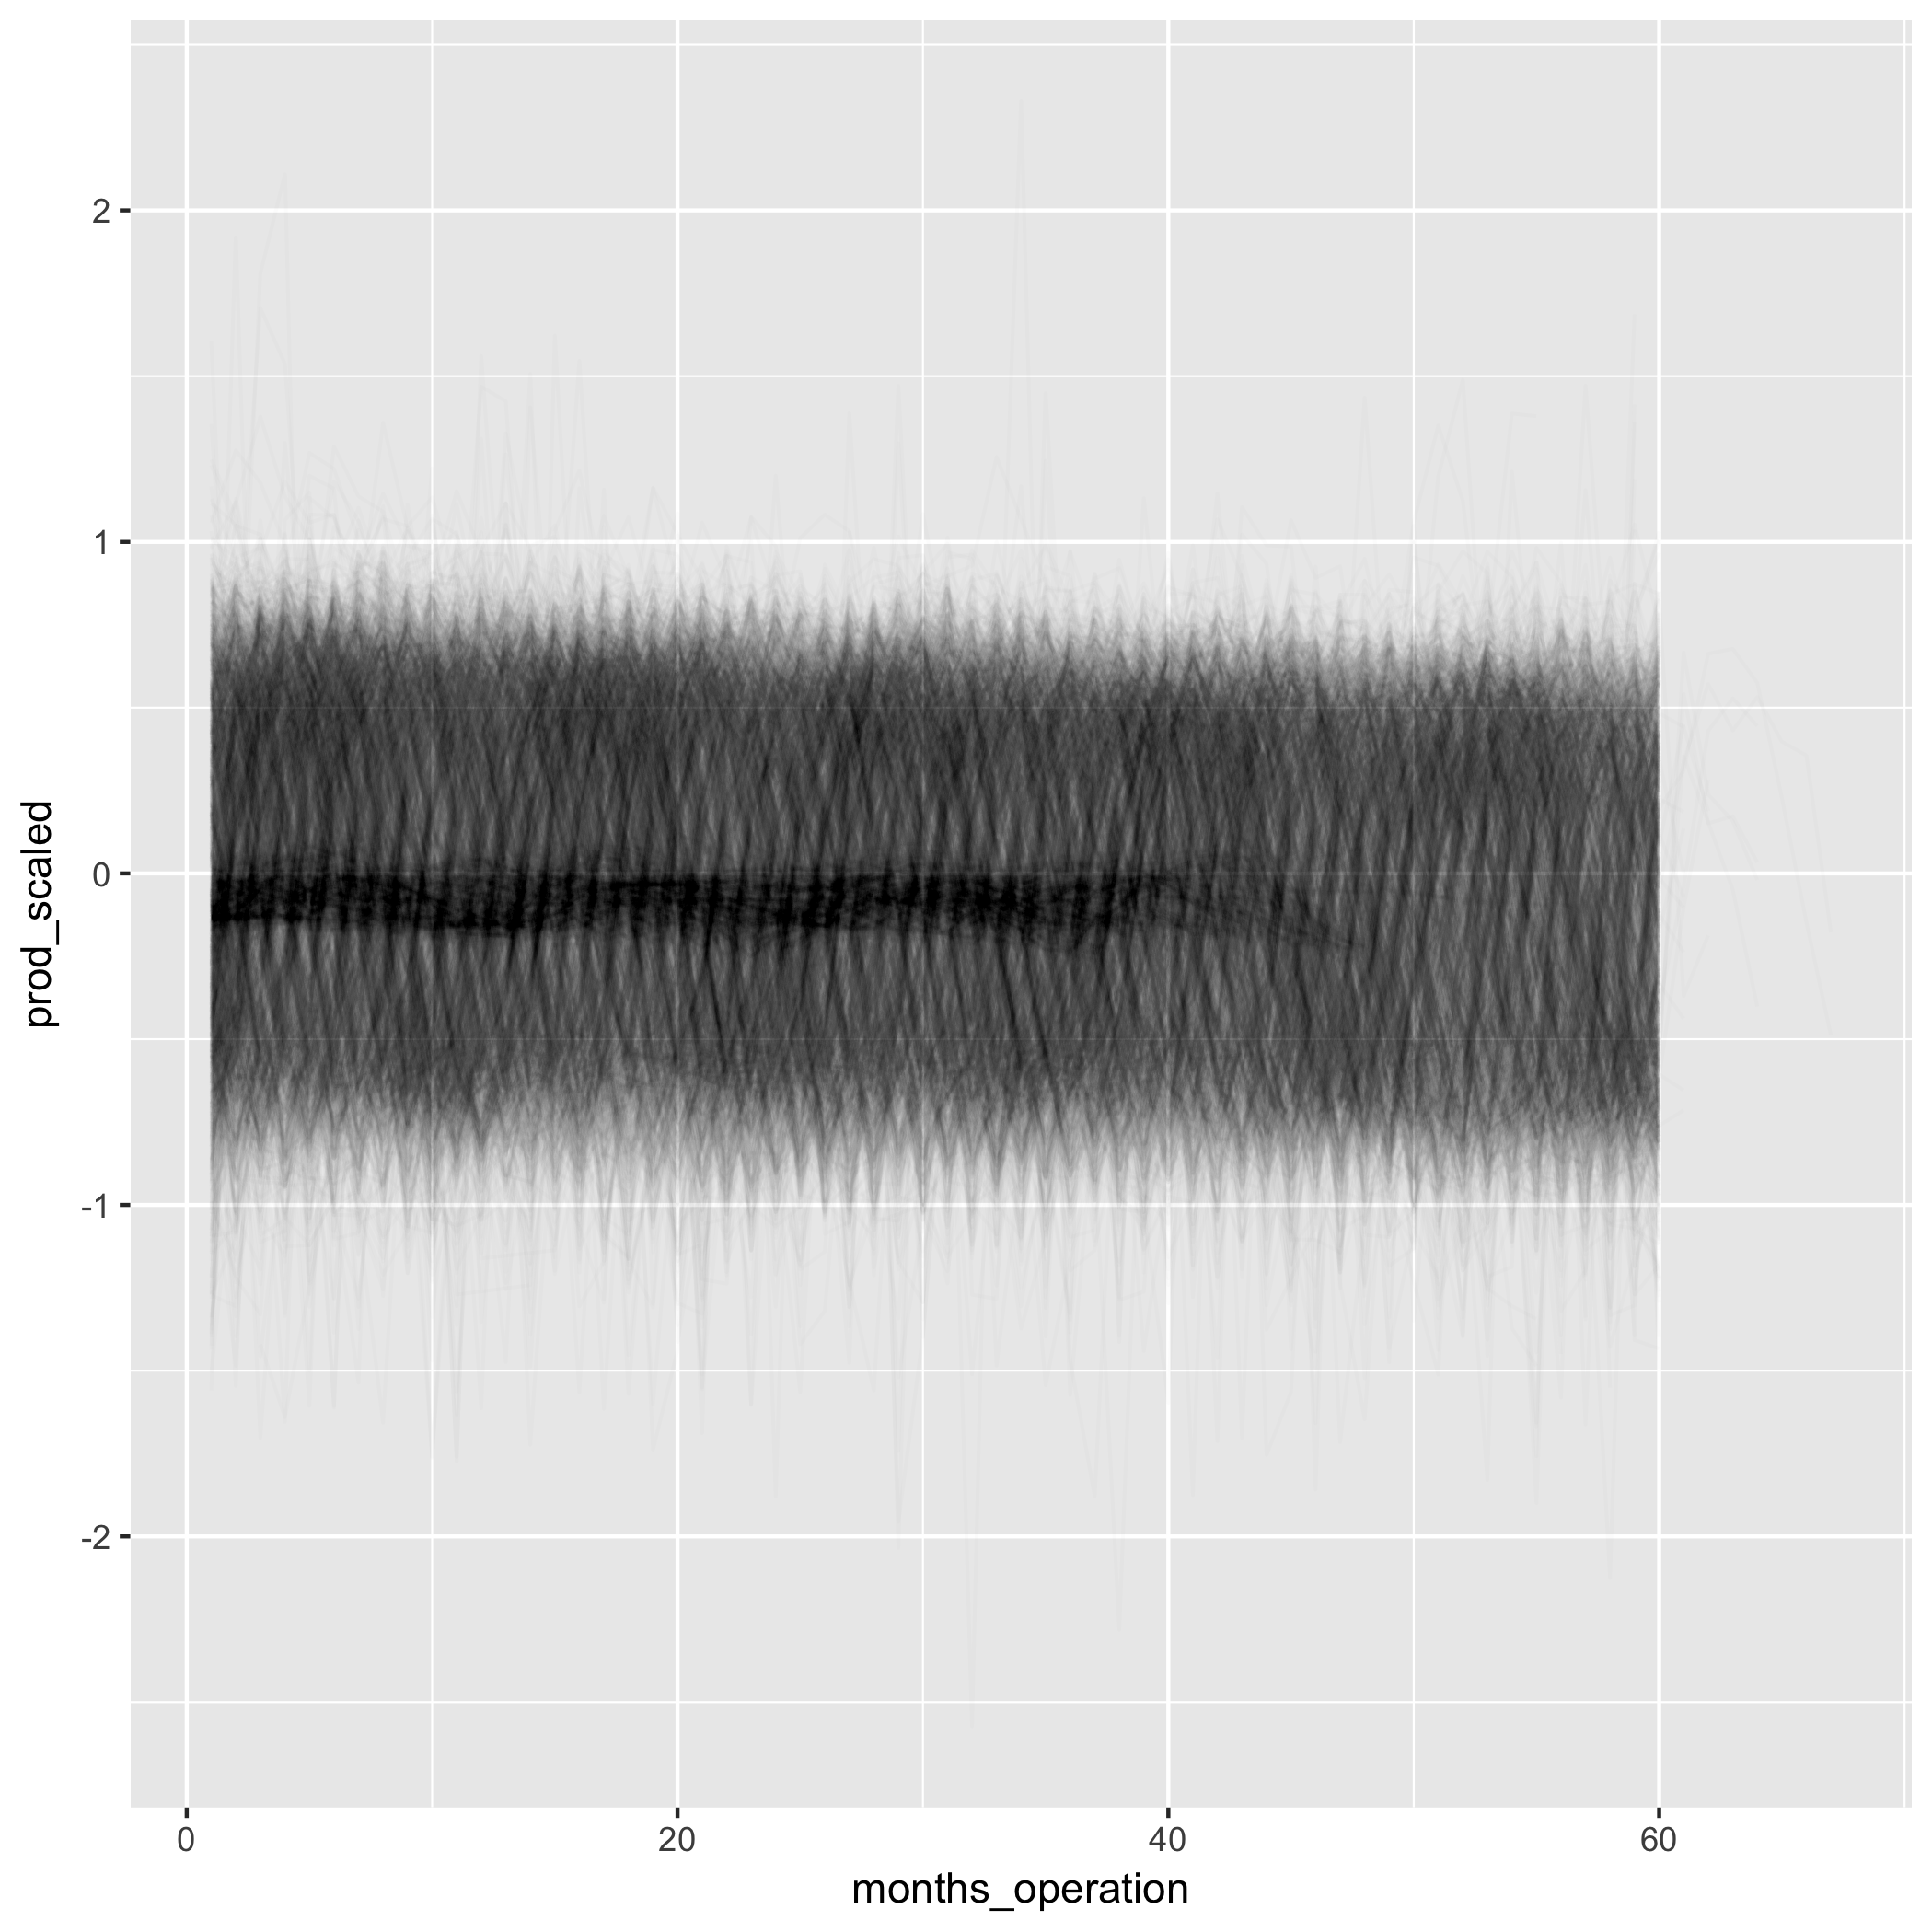
\includegraphics[width=1\linewidth]{figures/production.png}
  \caption{The figure shows the de-scaled production over time from the sample of solar panel systems. The red line represents the average degradation over time for all panels.}
  \label{fig:production}
\end{figure}

Month-of-year dummy variables are used to control for the seasonality in the data. The capacity of the solar panel system is the actual maximum capacity of a solar power system as reported to and audited by the CSI. This can be somewhat lower than the total nameplate capacity of the solar panels, and can depend on not only the technical capacity of the panels, but also on supporting equipment, such as the inverter, and factors such as the angle of the roof and orientation of the solar panel system.

The cost per kilowatt (\$/kW) variable is the reported total cost of the solar panel system divided by the CSI capacity rating. For solar panel systems that are sold outright, the total cost is simply the transaction price of the entire system. For systems with third party owners, the total cost is an estimate reported by the system owner based on the sum of component costs, installation costs and a mark-up. I will discuss how this may effect the results.

In the analysis I distinguish between solar panels that are host-owned and those that are third-party owned, which I refer to as being leased. What I refer to as leased can however take two main forms. The most common is a Power Purchase Agreement (PPA) where the host agrees to buy the electricity from the solar panel system for an agreed upon price, (which may increase at an agreed upon rate over time). Alternatively, a host may pay a flat monthly fee for the electricity produced by the solar panel.

Finally, among the 3000 plus solar power systems, 497 had residential owners, 1759 had commercial owners, 777 had governmental owners and 112 had non-profit owners. A portion of the commercial owners operate as third-party-owners, with hosts in the other sectors. Alternatively, I could include host sector in my analysis: 1241 solar panel systems had a commercial host, 501 had a residential host, 1199 had a governmental host and 204 had a non-profit host. However, In a study of asymmetric information, it makes most sense to focus on the sector of the owner.


\section{Linear Mixed Effects Models Estimated by Maximum Likelihood}

\subsection{Testing for differences between module manufacturer}
Following the notation of \citet{bates_fitting_2015}, the conditional distribution of the response variables, $y$ in a linear mixed effects model can be written compactly as in equation \ref{equation:lme_simple}. Here $\mathbf{\beta}$ is a p-dimensional coefficient vector (or  ``fixed effects'') of the $n \times p$ matrix $\mathbf{X}$ of (p-1) explanatory variables plus intercept term. $\mathbf{Z}$ is an $n \times q$ model matrix of the variables whose groups are to be modeled directly with corresponding vector of coefficients, or ``random effects'' $\mathbf{B}$ that are fixed at values $\mathbf{b}$.\footnote{The use of ``random'' refers to the fact that these groups are assumed to be specific to the sample. Many applications of mixed effects model thus treat the varying group coefficients as group-level error-terms. Interpreting coefficients as group varying coefficients or as group error terms is mathematically equivalent.} Here $q$ is a dependent on the number of terms, $k$, that are allowed to vary by group and the number of groups, $l$ for each term: $q=\sum_i^k q_i = \sum_i^k l_i p_i$.  $\mathbf{W}$ is a diagonal matrix of known prior weights. $B$ is distributed as multinomial normal with zero mean and where $\Sigma$ is variance-covariance matrix.

\begin{align}
(y|\mathbf{B=b}) &\sim \mathcal{N}(\mathbf{X\beta + Zb}, \sigma^2\mathbf{W^{-1}})\\
B &\sim \mathcal{N}(\mathbf{0,\Sigma})
\label{equation:lme_simple}
\end{align}

Models of this form can be solved efficiently using a penalized maximum likelihood routine. For further details of both the model and routine, I refer to \citet{bates_fitting_2015}.

To test whether I can detect quality differences between module manufacturers, I need to first estimate a restricted comparison model. I write the restricted comparison model explicitly in equation \ref{eqn:observation_level_rest}.

In this model, the transformed production variable, $prod\_scaled_{i}$ for observation $i$ is distributed normally with the mean modeled as a linear function of an intercept term $a_s$, a slope term, $b_s$ on the transformed months of operation variable $months\_operation\_scaled$, and a set of dummy variables representing the month of year, $\mathbf{month}$. Notice that the intercept and slope are indexed by $s$, indicating that they are allowed to vary by the individual system. Thus in this model formulation I take into account the groupings by system, explicitly modeling varying relative initial production values (intercepts) and degradation over time (slope). Moving up a level, the estimated $a$ and $b$ parameters are in turn modeled as multivariate normal.

\begin{equation}
\begin{aligned}
prod_{i} &\sim N(\mathbf{month} + a_s + b_s months\_operation\_scaled_{i}, \sigma^2)\\
\begin{pmatrix}
  a\\
  b
\end{pmatrix}
&\sim N
\begin{pmatrix}
  \mu_a\\
  \mu_b
\end{pmatrix},
\begin{pmatrix}
  \sigma_a^2 & \rho \sigma_a \sigma_b \\
  \rho \sigma_a \sigma_b & \sigma_b^2
\end{pmatrix}\label{eqn:observation_level_rest}
\end{aligned}
\end{equation}

The inclusion of the matrix of month dummies, $\mathbf{\mu^{month}}$, controls for seasonal variation across all systems. This is a simplified way to model seasonality, but because the data is itself at a monthly frequency, and a more direct modeling of seasonality is not of direct importance, this should suffice. As long as un-modeled variation in seasonality is not correlated with the long-run slope of production, the point estimates for the slope should be unbiased.

To test whether quality varies among module manufacturers, I simply add panel manufacturer as an extra hierarchy to the model. In this model, the observation-level regression is identical to the restricted comparison model as in equations \ref{eqn:observation_level_rest}. The system-level intercepts, $a$, and slopes, $b$, terms are also modeled as multivariate normal. But the mean values of the multivariate normal distribution, $\mu_a$ and $\mu_b$, are now indexed by $m$, as shown in equation \ref{eqn:unrest}, representing that they are allowed to vary by module manufacturer.

\begin{equation}
\begin{aligned}
\begin{pmatrix}
  a\\
  b
\end{pmatrix}
&\sim N \Bigg(
\begin{pmatrix}
  \mu_{a[m]}\\
  \mu_{b[m]}
\end{pmatrix},
\begin{pmatrix}
  \sigma_{a[m]}^2 & \rho \sigma_{a} \sigma_{b} \\
  \rho \sigma_a \sigma_b & \sigma_b^2
\end{pmatrix} \Bigg) \\
\mu_{a} &\sim N(\theta_a, \sigma_{\mu_a}^2) \\
\mu_{b} & \sim N(\theta_b, \sigma_{\mu_b}^2) \label{eqn:unrest}
\end{aligned}
\end{equation}

If there is no significant variation between the module manufacturer groupings, this model collapses into the restricted comparison model, which is the null hypothesis. Figure \ref{sfig:sys_slope_fig} gives a visual summary of the system-level slope terms ordered from lowest to highest. The lines represent approximate 95\% confidence intervals around the point estimates. One anomaly we can notice is that a handful of the systems have slopes that are estimated to be positive. This is clearly problematic if we wish to interpret the slope coefficient as degradation over time. I address this in the full Bayesian model without resorting to excluding data.

\begin{figure}
  \caption{Approximate 95\% confidence intervals around maximum likelihood point estimates of system-level slope terms, $b_i$, ordered from lowest to highest. Visually, we can see significant differences in the average degradation over time across solar power systems.}
  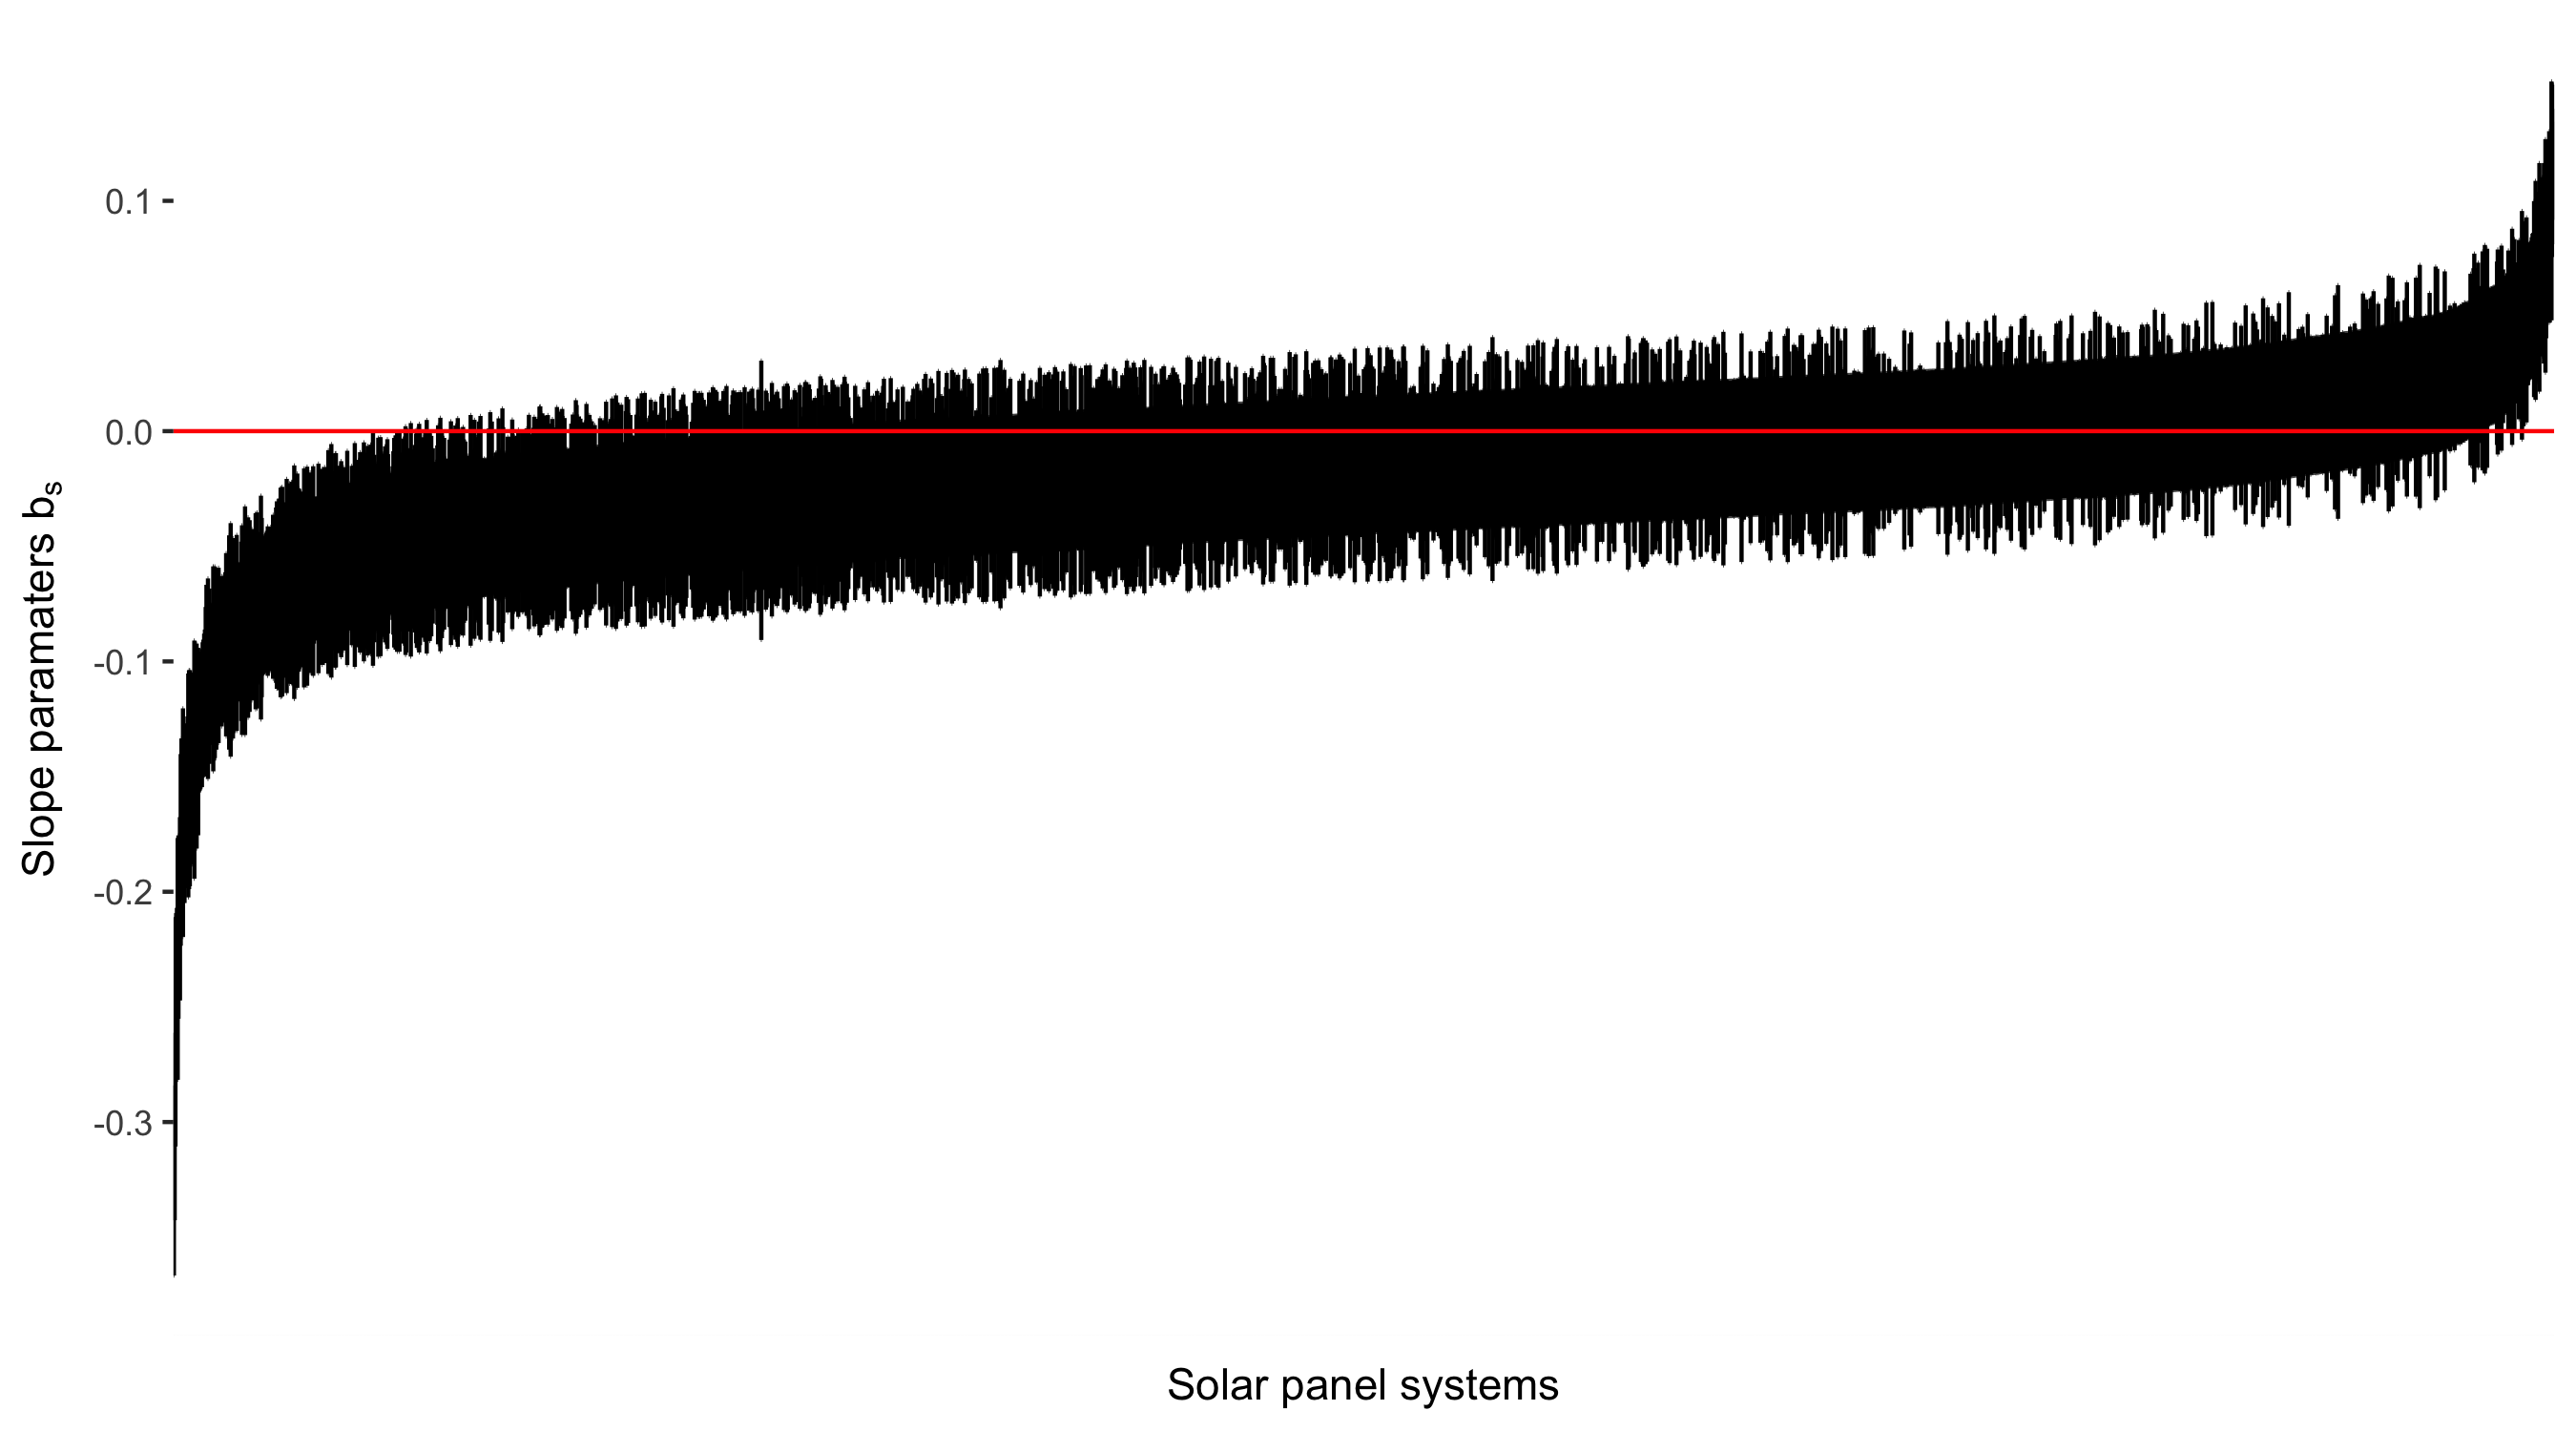
\includegraphics[width=1\linewidth]{figures/sys_slope_fig.png}
  \label{sfig:sys_slope_fig}
\end{figure}

Figure \ref{sfig:nested_manuf_fig} gives a summary of the estimated manufacturer-level mean slopes. Again the lines represent 95\% confidence intervals around the point estimates. Visually, we can see substantial variation in quality between the manufacturer groups. We can formally test the hypothesis that manufacturer groupings improve the explanatory power of the model with a comparison to the restricted model with a likelihood ratio test. The results are shown in table \ref{tbl:lm_commodity}. The information criteria measures (AIC, BIC) are both lower, indicating better predictive power of the model with manufacturer groupings. The Chi-square statistic indicates that the model with manufacturer groupings substantially improves model performance.

\begin{figure}
  \caption{Approximate 95\% confidence intervals around maximum likelihood estimators of manufacturer-level mean slope terms $\mu_b$, ordered from lowest to highest. These are the means of the higher level normal distributions that vary by manufacturer that the system-level parameters are assumed to be drawn from. The visual impression is of substantial variation between manufacturer groupings.}
  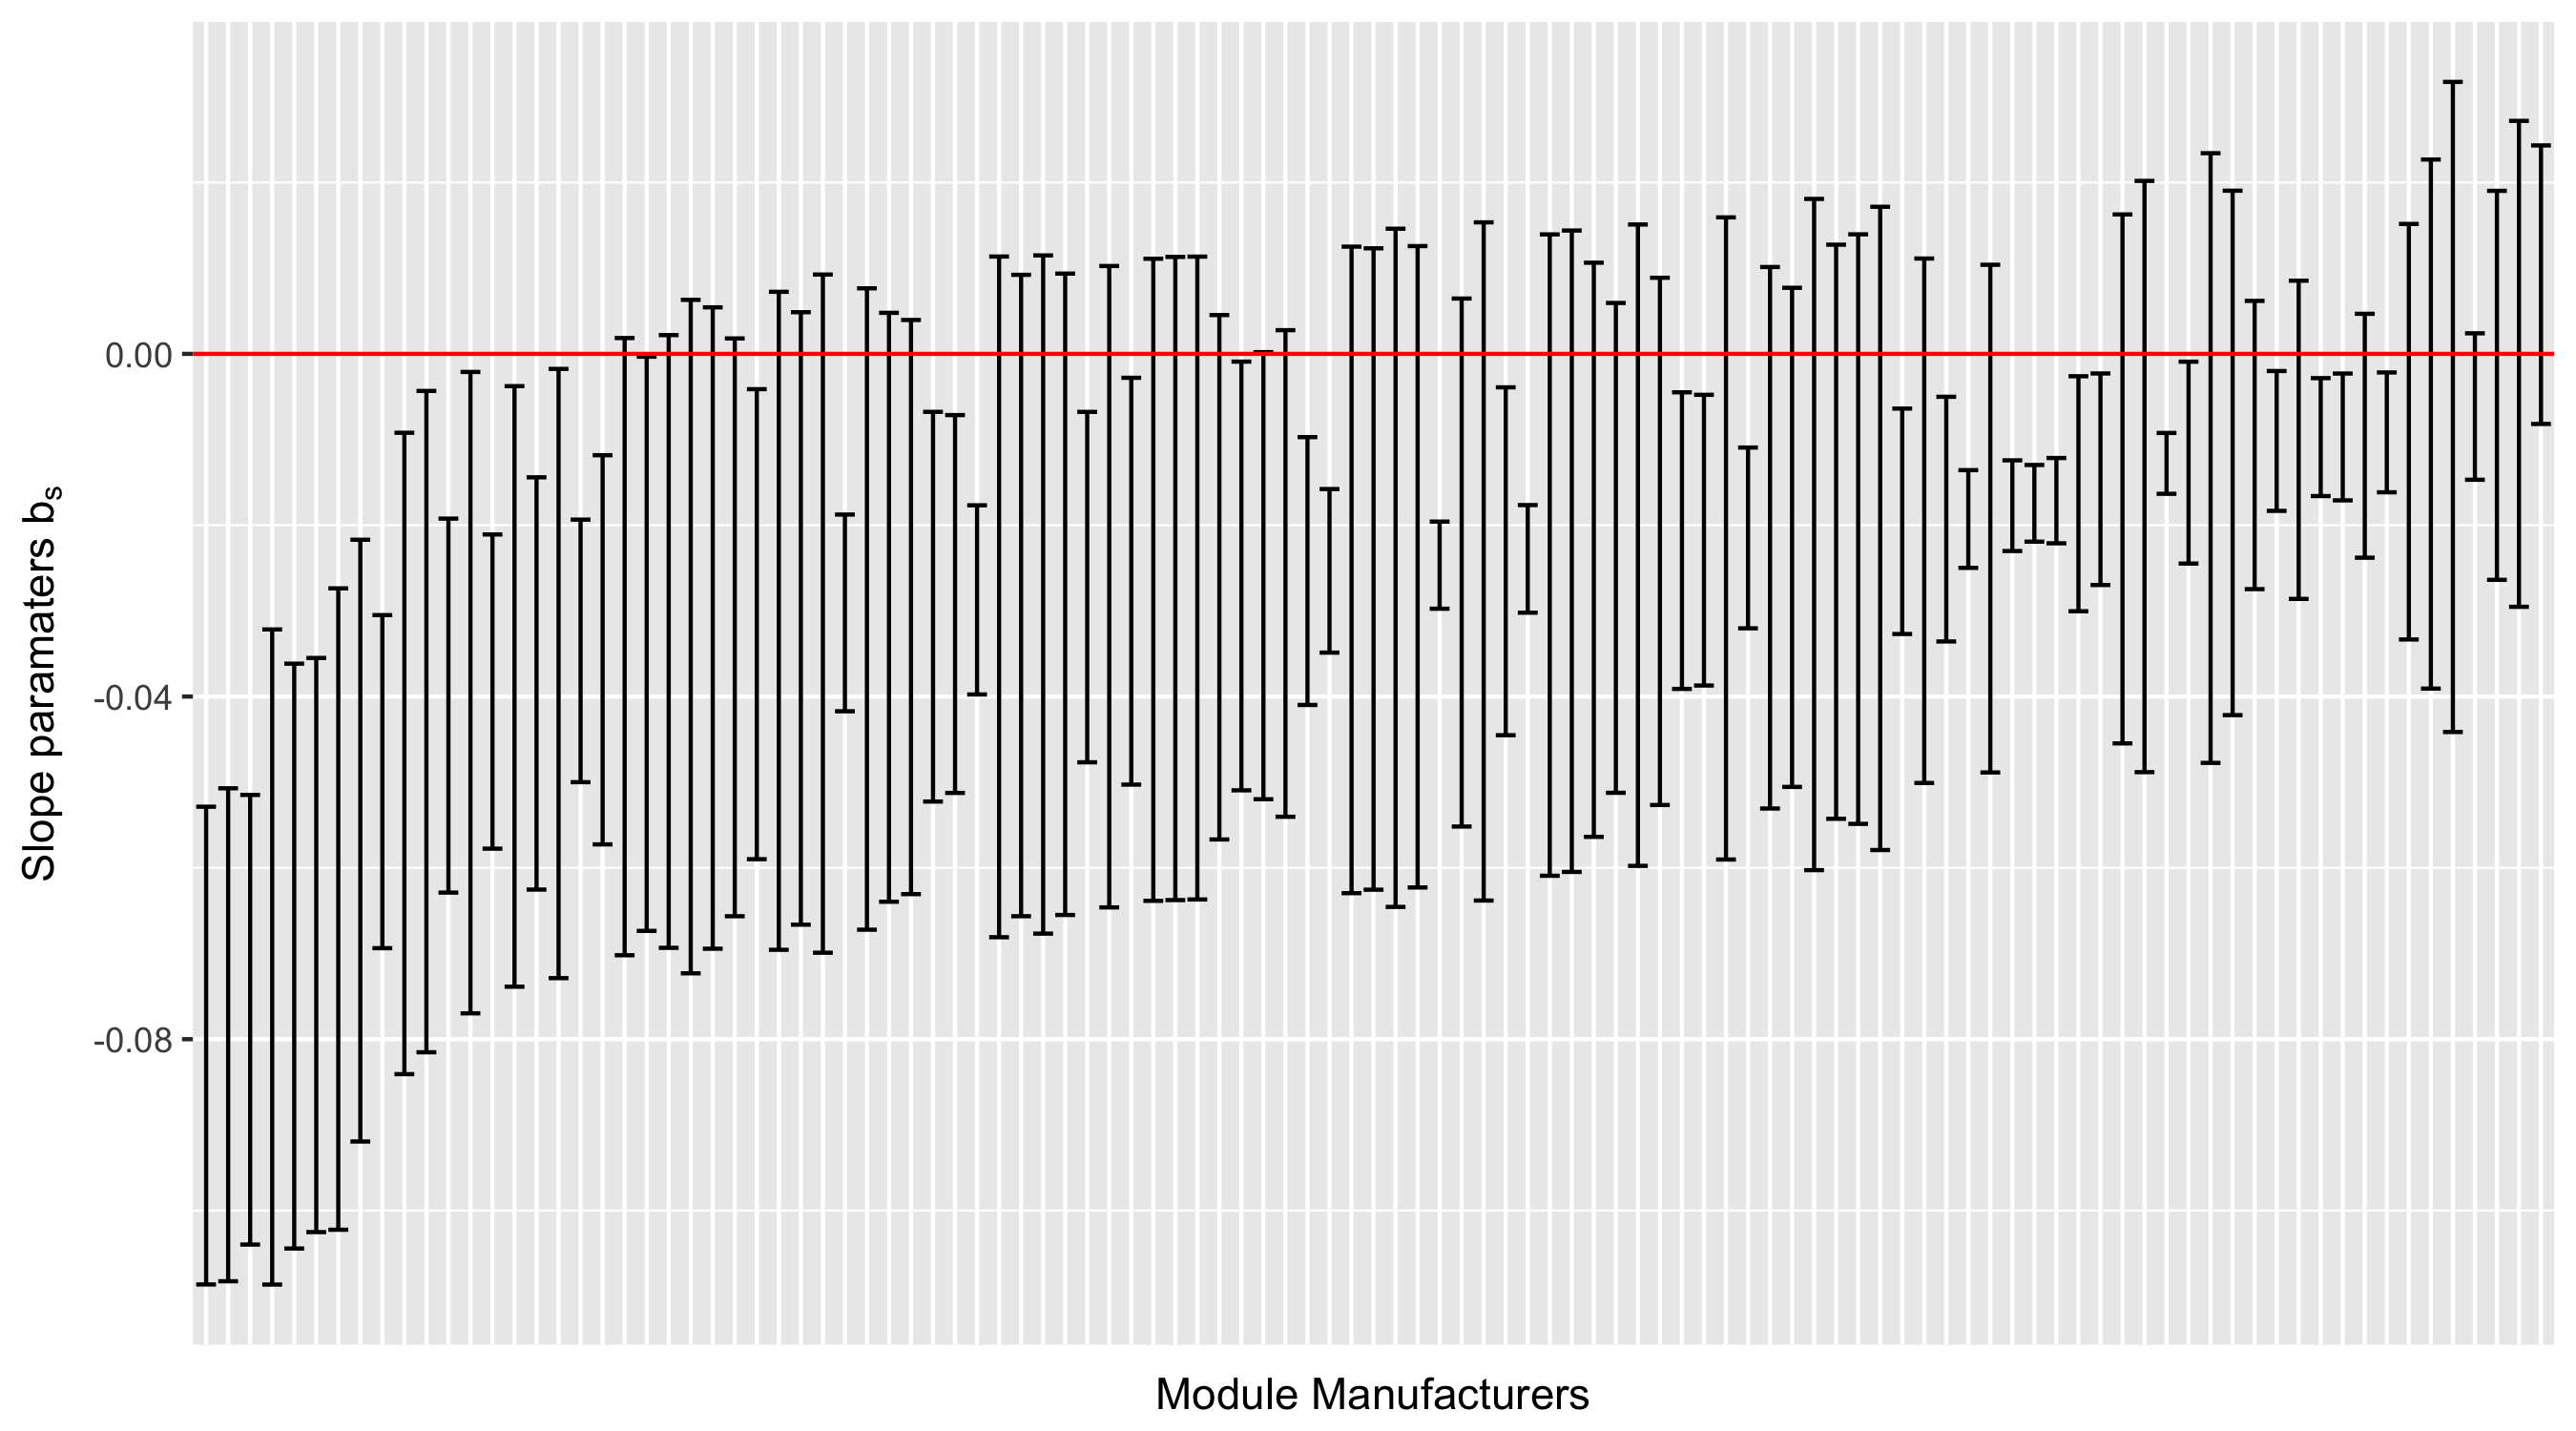
\includegraphics[width=1\linewidth]{figures/nested_manuf_fig_final.png}
  \label{sfig:nested_manuf_fig}
\end{figure}

\begin{table}
  \begin{tabular}{rllllllll}
  \toprule
    Model &  DF &   AIC &   BIC &  logLik &  deviance &  Chisq &  Chi df &  $Pr(>Chisq)$ \\
    \midrule
             Restricted &  17 &  8805 &  8976 &   -4385 &      8771 &     -- &      -- &          -- \\
    Grouped Manuf. &  20 &  8430 &  8631 &   -4195 &      8390 &    381 &       3 &     2.6e-82 \\
  \bottomrule
  \end{tabular}
  \label{tbl:lm_commodity}
  \caption{A likelihood ratio test indicates that the addition of panel manufacturer as a hierarchy significantly improves the predictive power of the model. Akaike Information Criterion (AIC) and Bayesian Information Criterion are lower in the model with manufacturer groupings, indicating better out-of-sample predictive fit.}
\end{table}

The first result, of which the evidence appears to be quite strong, is that solar panel systems do appear to vary substantially in quality between module manufacturers. Given that module quality is a salient differentiating characteristic between panels, it is then difficult to view solar panels as commodities.

\subsection{Testing for asymmetric information: differences in quality between leased and host-owned solar power systems}

Provided the evidence that solar panel systems are not commodities and that substantial differences in quality do exist between manufacturers, we can now move on to the testable implication that comes from a combination of standard economic theory of asymmetric information and a descriptive understanding of the market that suggests solar panels could be subject to issues of asymmetric information of quality.

From our informal model of asymmetric information where we see host owners of solar systems as being low-information types, while owners of leased panels as being high-information types, we would predict that on average leased panels will display higher quality over time. To test this directly with the data, I only need to do a slight modification of the model in the previous subsection. Instead of grouping the system-level coefficients by manufacturer, I now group into whether the solar power system was leased or not, as indexed by $l$. We can then compare the average slopes between these groups. For convenience the model is presented in full in equations \ref{eqn:fullmodel}.

\begin{equation}
\begin{aligned}
log_prod_{i} &\sim N(\mathbf{month} + a_s + b_s months\_operation\_scaled_{i}, \sigma^2)\\
\begin{pmatrix}
  a\\
  b
\end{pmatrix}
&\sim N \Bigg(
\begin{pmatrix}
  \mu_{a[l]}\\
  \mu_{b[l]}
\end{pmatrix},
\begin{pmatrix}
  \sigma_{a}^2 & \rho \sigma_{a} \sigma_{b} \\
  \rho \sigma_a \sigma_b & \sigma_b^2
\end{pmatrix} \Bigg) \\
\mu_{a} &\sim N(\theta_a, \sigma_{\mu_a}^2) \\
\mu_{b} & \sim N(\theta_b, \sigma_{\mu_b}^2) \label{eqn:fullmodel}
\end{aligned}
\end{equation}

A visual summary of the results are shown in figure \ref{lease_sys_fig}. Again, the vertical lines represent approximate 95\% confidence intervals over the point estimates for the system-level slope terms, $b_s$. But here the the slope estimates are grouped into host-owned (left) and leased (right). The estimated group means are shown as horizontal lines. At the scale of the figure, the effect appears small, but the average slopes are estimated to be significantly different from each other at the 95\% confidence interval. The difference is also economically significant. Extrapolating out from the difference in the point estimates between leased and host-owned panels suggests that on average a leased system can expect to be producing 11\% more power after 10 years compared to an otherwise similar solar panel system that is host-owned.

\begin{figure}
  \centering
	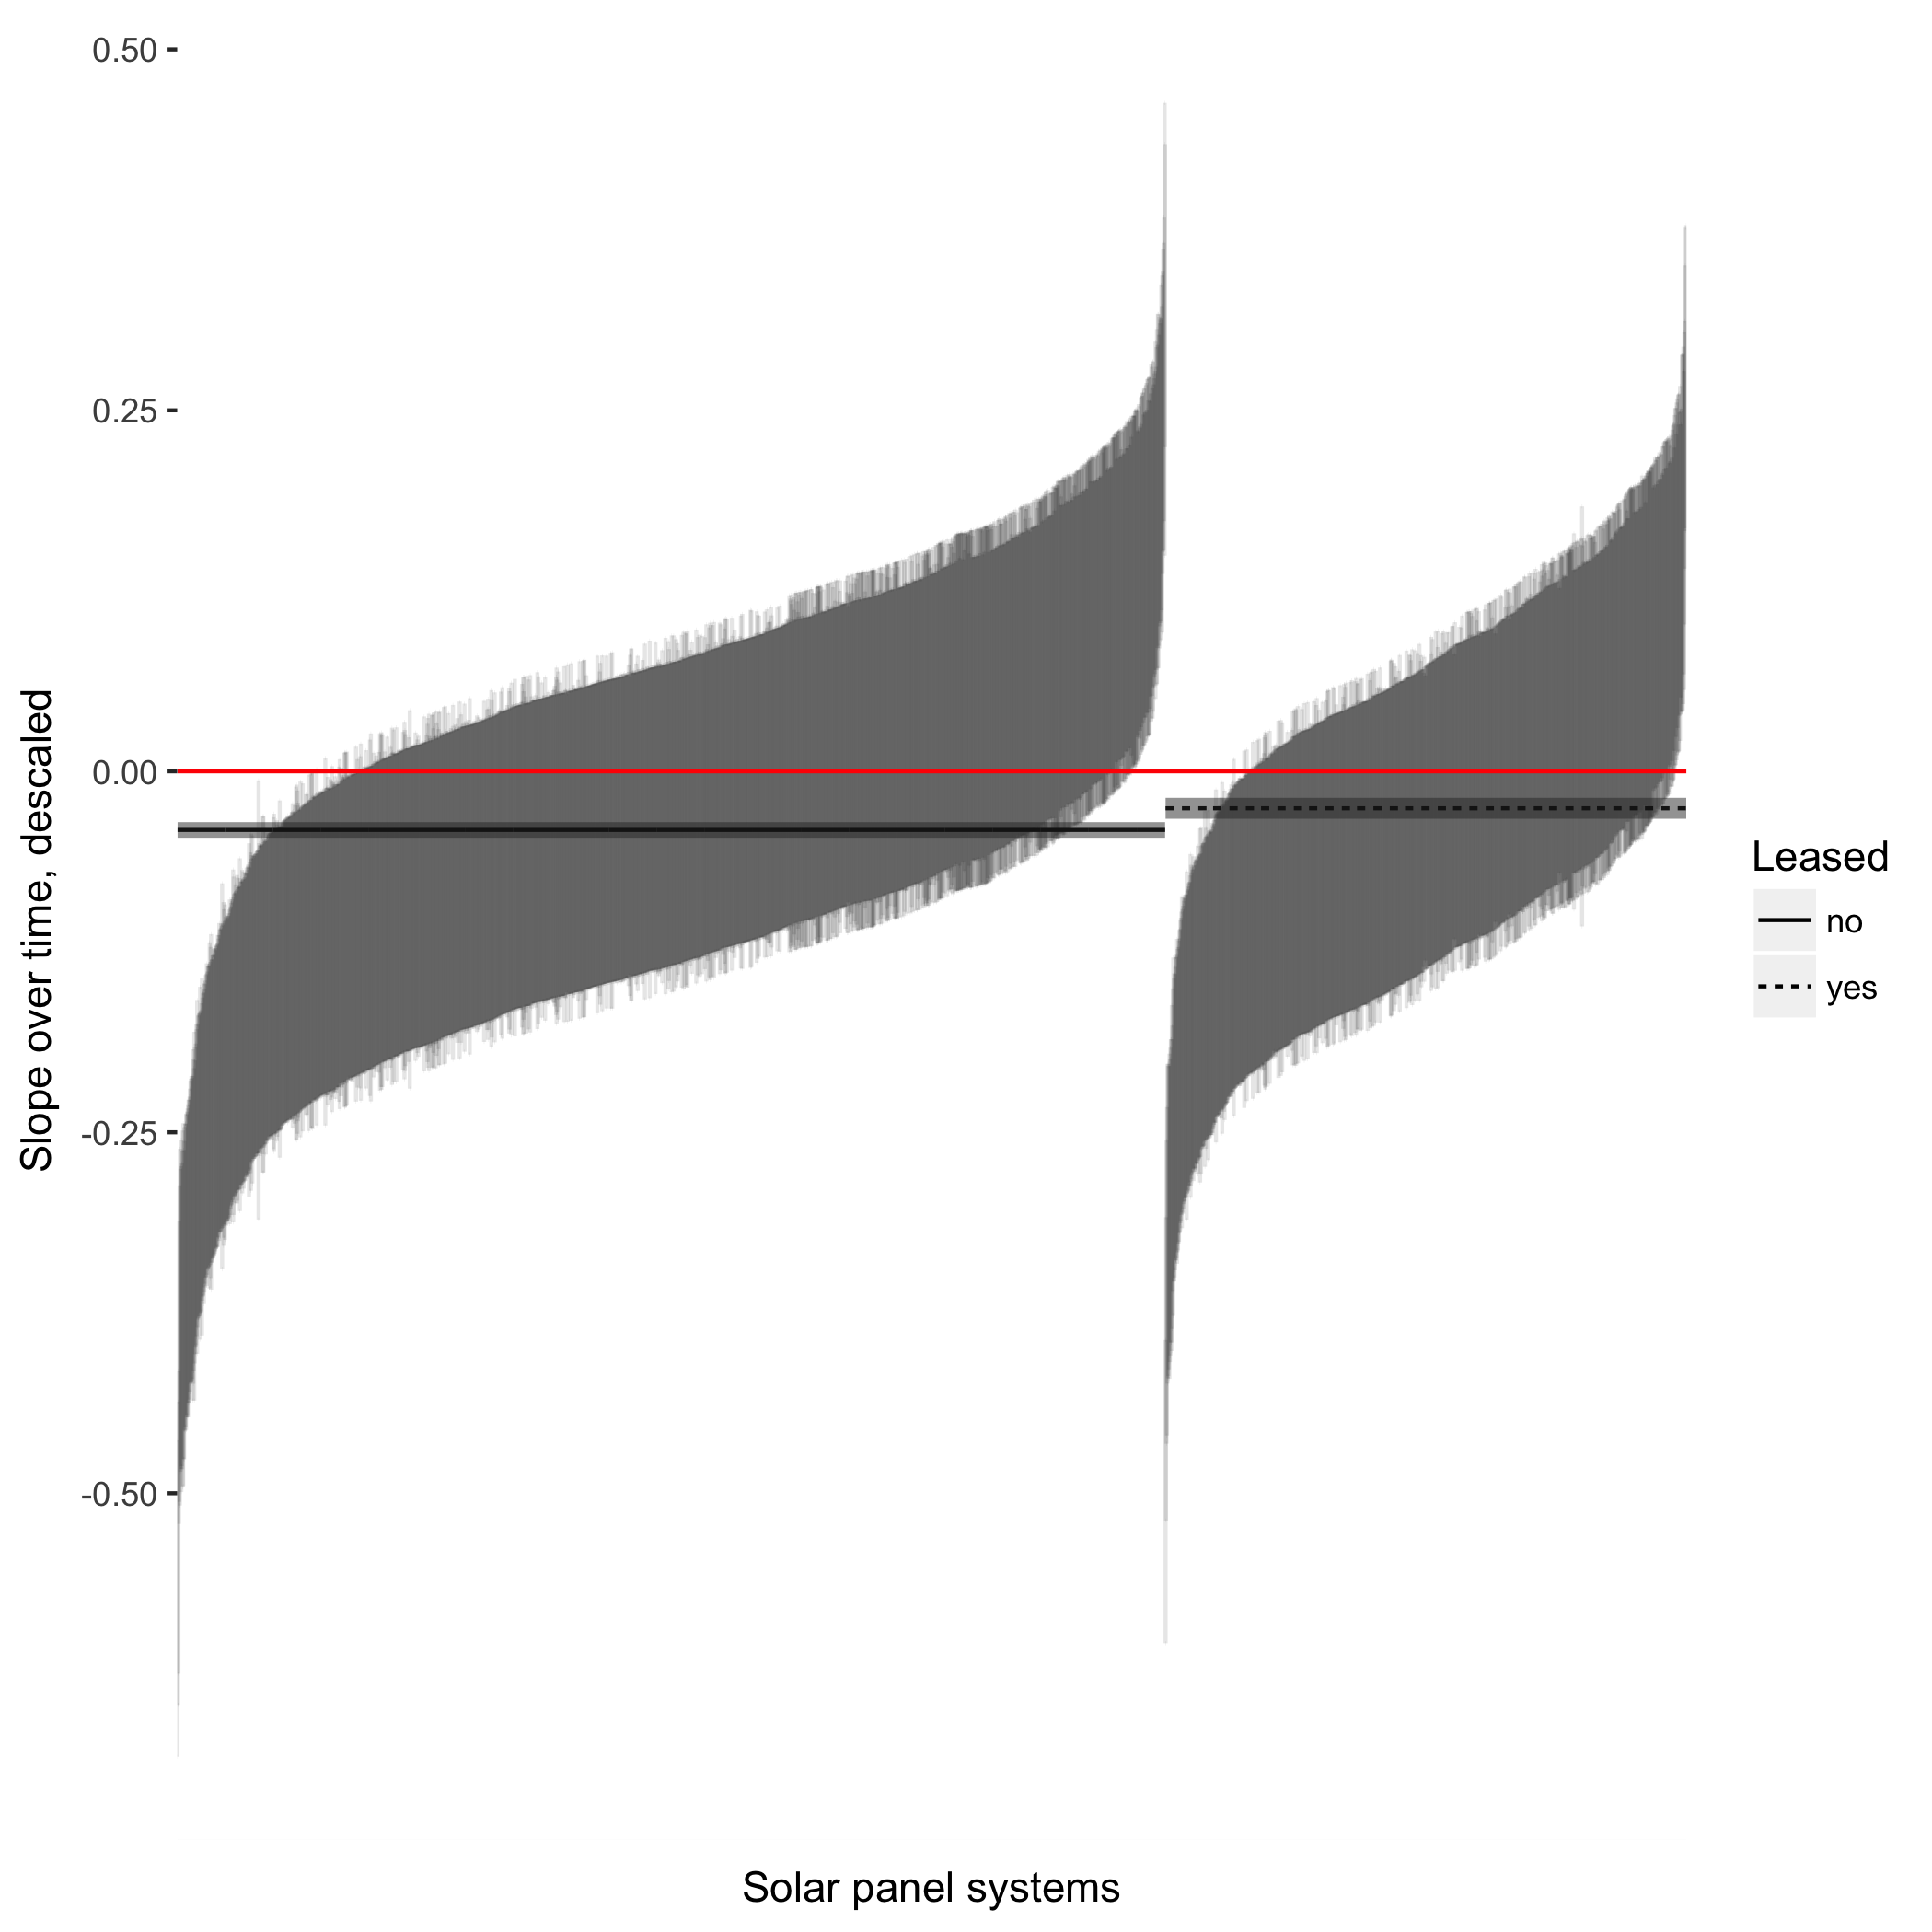
\includegraphics[width=1\textwidth]{figures/lease_sys_fig.png}
	\caption{A visual summary of the estimation results where panels are grouped by owner type: leased (high information third-party owner) or host-owned (low information owner). The vertical lines again represent 95\% confidence interval on the estimated system-level slope coefficients, which are sorted first by ownership type (host-owned on the left, leased on the right), and then from low to high of the maximum likelihood point estimate of the slope estimates. The red line represents the zero threshold. The horizontal black line on the left represents the mean of the higher level distribution on the slopes for host-owned systems, $\mu_b[l=0]$, while the dotted black line on the right represents the mean of the higher level distribution on the slopes for third-party owned systems, $\mu_b[l=1]$ }
	\label{lease_sys_fig}
\end{figure}

\section{Full Bayesian hierarchical model}
Up until now, I have used relatively parsimonious models with few fixed-effects and only one or two hierarchies ("random effects").  Ideally, I would like to estimate a full probability model with all relevant and available covariates and hierarchies. First and foremost so that the parameters of interests to the testable implications can be estimated simultaneously from one model. But also, as \citet{barr_random_2013} shows, mixed-effects models that have the maximum random effects structure justified by the model, provide the best out-of-sample prediction. Estimating mixed-effects models by maximum likelihood is efficient and straight-forward. However, convergence of the maximum likelihood routine is not guaranteed under richer models with more hierarchies and larger number of parameters to be estimated.

I wish to estimate a model where the variable for cost per-kW is included as an interaction that varies by system and module manufacturer. I also wish to have a model where both system, module manufacturer, and leasing hierarchies are estimated simultaneously. Geographic information on the location of solar panels could also conceivably be correlated with degradation of solar panels, and should be accounted for in the model.  I am not able to obtain convergence of the maximum likelihood routines under this rich model.

As a solution, I build a fully Bayesian hierarchical model\footnote{I purposefully change my nomenclature here and refer to the Bayesian model as a ``hierarchical mode'' to distinguish it from the models estimated by maximum likelihood, which I refer to as a linear mixed effects model. This distinction is mostly semantic. Both models resemble each other in structure. "hierarchical model" is however a broader term. There is no restriction to linearity. Models with non-linear or non-parametric components can also be incorporated and estimated.} estimated by Markov Chain Monte Carlo (MCMC) simulation techniques.

Multilevel models estimated using Bayesian techniques have some nice theoretical properties, as I discussed earlier. However, the main advantages to using the Bayesian techniques here are practical. Models of nearly arbitrary richness can be estimated, with computational time and available data being the main constraints. Inference is also well-defined and exact.\footnote{Exact in the sense that given a correctly specified probability model, then an MCMC routine that is given infinite time to sample, will in theory converge to the correct posterior probability distribution. Maximum likelihood is approximate in the sense that inference is based on asymptotic theory and assumptions of normality.}

A Bayesian MCMC approach has some additional attractive properties. Results are presented as estimates of marginal posterior distributions over coefficients of interest, which can be interpreted directly and intuitively as probabilities. Group-level variances are not constrained to be equal and assumptions of normality of the likelihood and posterior distributions can be loosened. For further discussion of the Bayesian frameworks and techniques, I refer to discussions in \citet{gelman_bayesian_2013}, \citet{kruschke_doing_2014}, or \citet{mcelreath_statistical_2015}.

The model is described by the equations in \ref{eqn:bayesMod}. The response variable is production data that has been de-scaled as described earlier. This response variable is given a normal likelihood with mean, $\hat{y}$ and standard deviation, $\sigma$. At the observation level, the fitted values, $\hat{y}$, are modeled as a simple linear regression, with an intercept $a_s$, and a slope $b_s$ which are both allowed to vary by system, $s$. In addition a vector of month dummies, $\mathbf{\mu^{month}}$ is included in order to control for seasonality.

At the system level, the intercept terms, $a_s$ are given a common higher level Cauchy distribution with location parameter $\mu^a$ and scale parameter $\sigma^a$. But because the intercept term is not of direct economic importance, it is not modeled further.

The slope terms, $b_s$ are also modeled as Normal distributions with mean $\mu^{b}_s$, that is allowed to vary by system, and standard deviation $\sigma^{b}$. I decompose the variation of $\mu^{b}_s$ into three terms that vary by lease, $\mu^{lease}_l$, host sector $\mu^{sect}_c$, and manufacturer $\mu^m_m$. In addition three continuous variables are included in the system-level equation: the year of first production, $first\_prod\_year_s$, capacity, $capacity_s$ and the system cost per kilowatt, $cost_s$ with corresponding coefficients $\beta^{fy}$, $\beta^{size}$, and $\beta^{cost}$.

\begin{equation}
\begin{aligned}
prod_{st} &\sim N(\hat{y}_{st}, \sigma)\\ %\label{eqn:likelihood}
\hat{y}_{st} &= a_s + b_s months\_operation_{st} + \mathbf{\mu^{month}}\\
a_s &\sim N(\mu^a, \sigma^a)  \label{eqn:bayesMod} \\
b_s &\sim N(\mu_s^b, \sigma^b) \\
\mu_{s}^{b} & = \mu^{lease}_l + \mu^{sect}_s + \mu^{manuf}_m + \mu^{county}_c  \\
& +\beta^{fy} first\_prod\_year_s + \beta^{size} log\_csi\_rating_s + \beta^{cost} log\_cost_s
\end{aligned}
\end{equation}

Higher level terms are all given Cauchy prior distributions as summarized in the equations in \ref{eqn:meta}. The Cauchy distribution, which is a T-distribution with 1 degree of freedom, has wide tails and thus allows for the occasional outlying coefficient in a lower level regression, while still provides some regularization towards zero \citep{gelman_weakly_2008}.

The $\mu^{lease}_l$, $\mu^{sect}_s$, and $\mu^{manuf}$ terms are all
modeled as coming from a Cauchy distribution with a location meta-parameter $\mu^{meta}$ and scale parameter $\sigma^{mu}$. Similarly, $\beta^{fy}$, $\beta^{size}$ and $\beta^{cost}_l$ are modeled as coming from a $Cauchy(\mu^{\beta}, \sigma^{\beta})$ distribution. The location parameters $\mu^{meta}$ and $\mu^{\beta}$ are in turn given a Cauchy(0,5) prior, while the corresponding $\sigma^{meta}$ and $\sigma^{beta}$ terms are given half-Cauchy(0,5) priors--essentially a Cauchy distribution constrained to the positive values.

The $Cauchy(0,5)$ prior is what is referred to as a weakly-informative prior. It imposes some weak regularization on the parameters, while also allowing for some outlying parameter estimates. At the same time, the prior does not impose any strong prior knowledge that meaningfully effects the posterior distribution, especially in the presence of substantial data. The parameters $\beta^{fy}$, $\beta^{size}$, $\beta^{cost}$ and $\mathbf{\mu^{month}}$ are all also given $Cauchy(0,5)$ prior distributions.

\begin{equation}
\begin{aligned}
\mu^{lease}_l &\sim Cauchy(\mu^{meta}, \sigma^{\mu}) \\
\mu^{sect}_s &\sim Cauchy(\mu^{meta}, \sigma^{\mu}) \\
\mu^{manuf}_m &\sim Cauchy(\mu^{meta}, \sigma^{\mu}) \label{eqn:meta} \\
\mu^{meta} &\sim Cauchy(0, 5) \\
\mu^{a} &\sim Cauchy(0,5) \\
\mathbf{\mu^{month}} &\sim Cauchy(0,5) \\
\beta^{fy} &\sim Cauchy(\mu^{\beta}, \sigma^{\beta}) \\
\beta^{size} &\sim Cauchy(\mu^{\beta}, \sigma^{\beta})\\
\beta_l^{cost} &\sim Cauchy(\mu^{\beta}, \sigma^{\beta})\\
\mu^{\beta} &\sim Cauchy(0, 5) \\
\sigma &\sim half-Cauchy(0,5) \\
\sigma^{a} &\sim half-Cauchy(0,5) \\
\sigma^{b} &\sim half-Cauchy(0,5) \\
\sigma^{\mu} &\sim half-Cauchy(0,5)\\
\sigma^{\beta} &\sim half-Cauchy(0,5)\\
\end{aligned}
\end{equation}

\begin{figure}
  \centering
	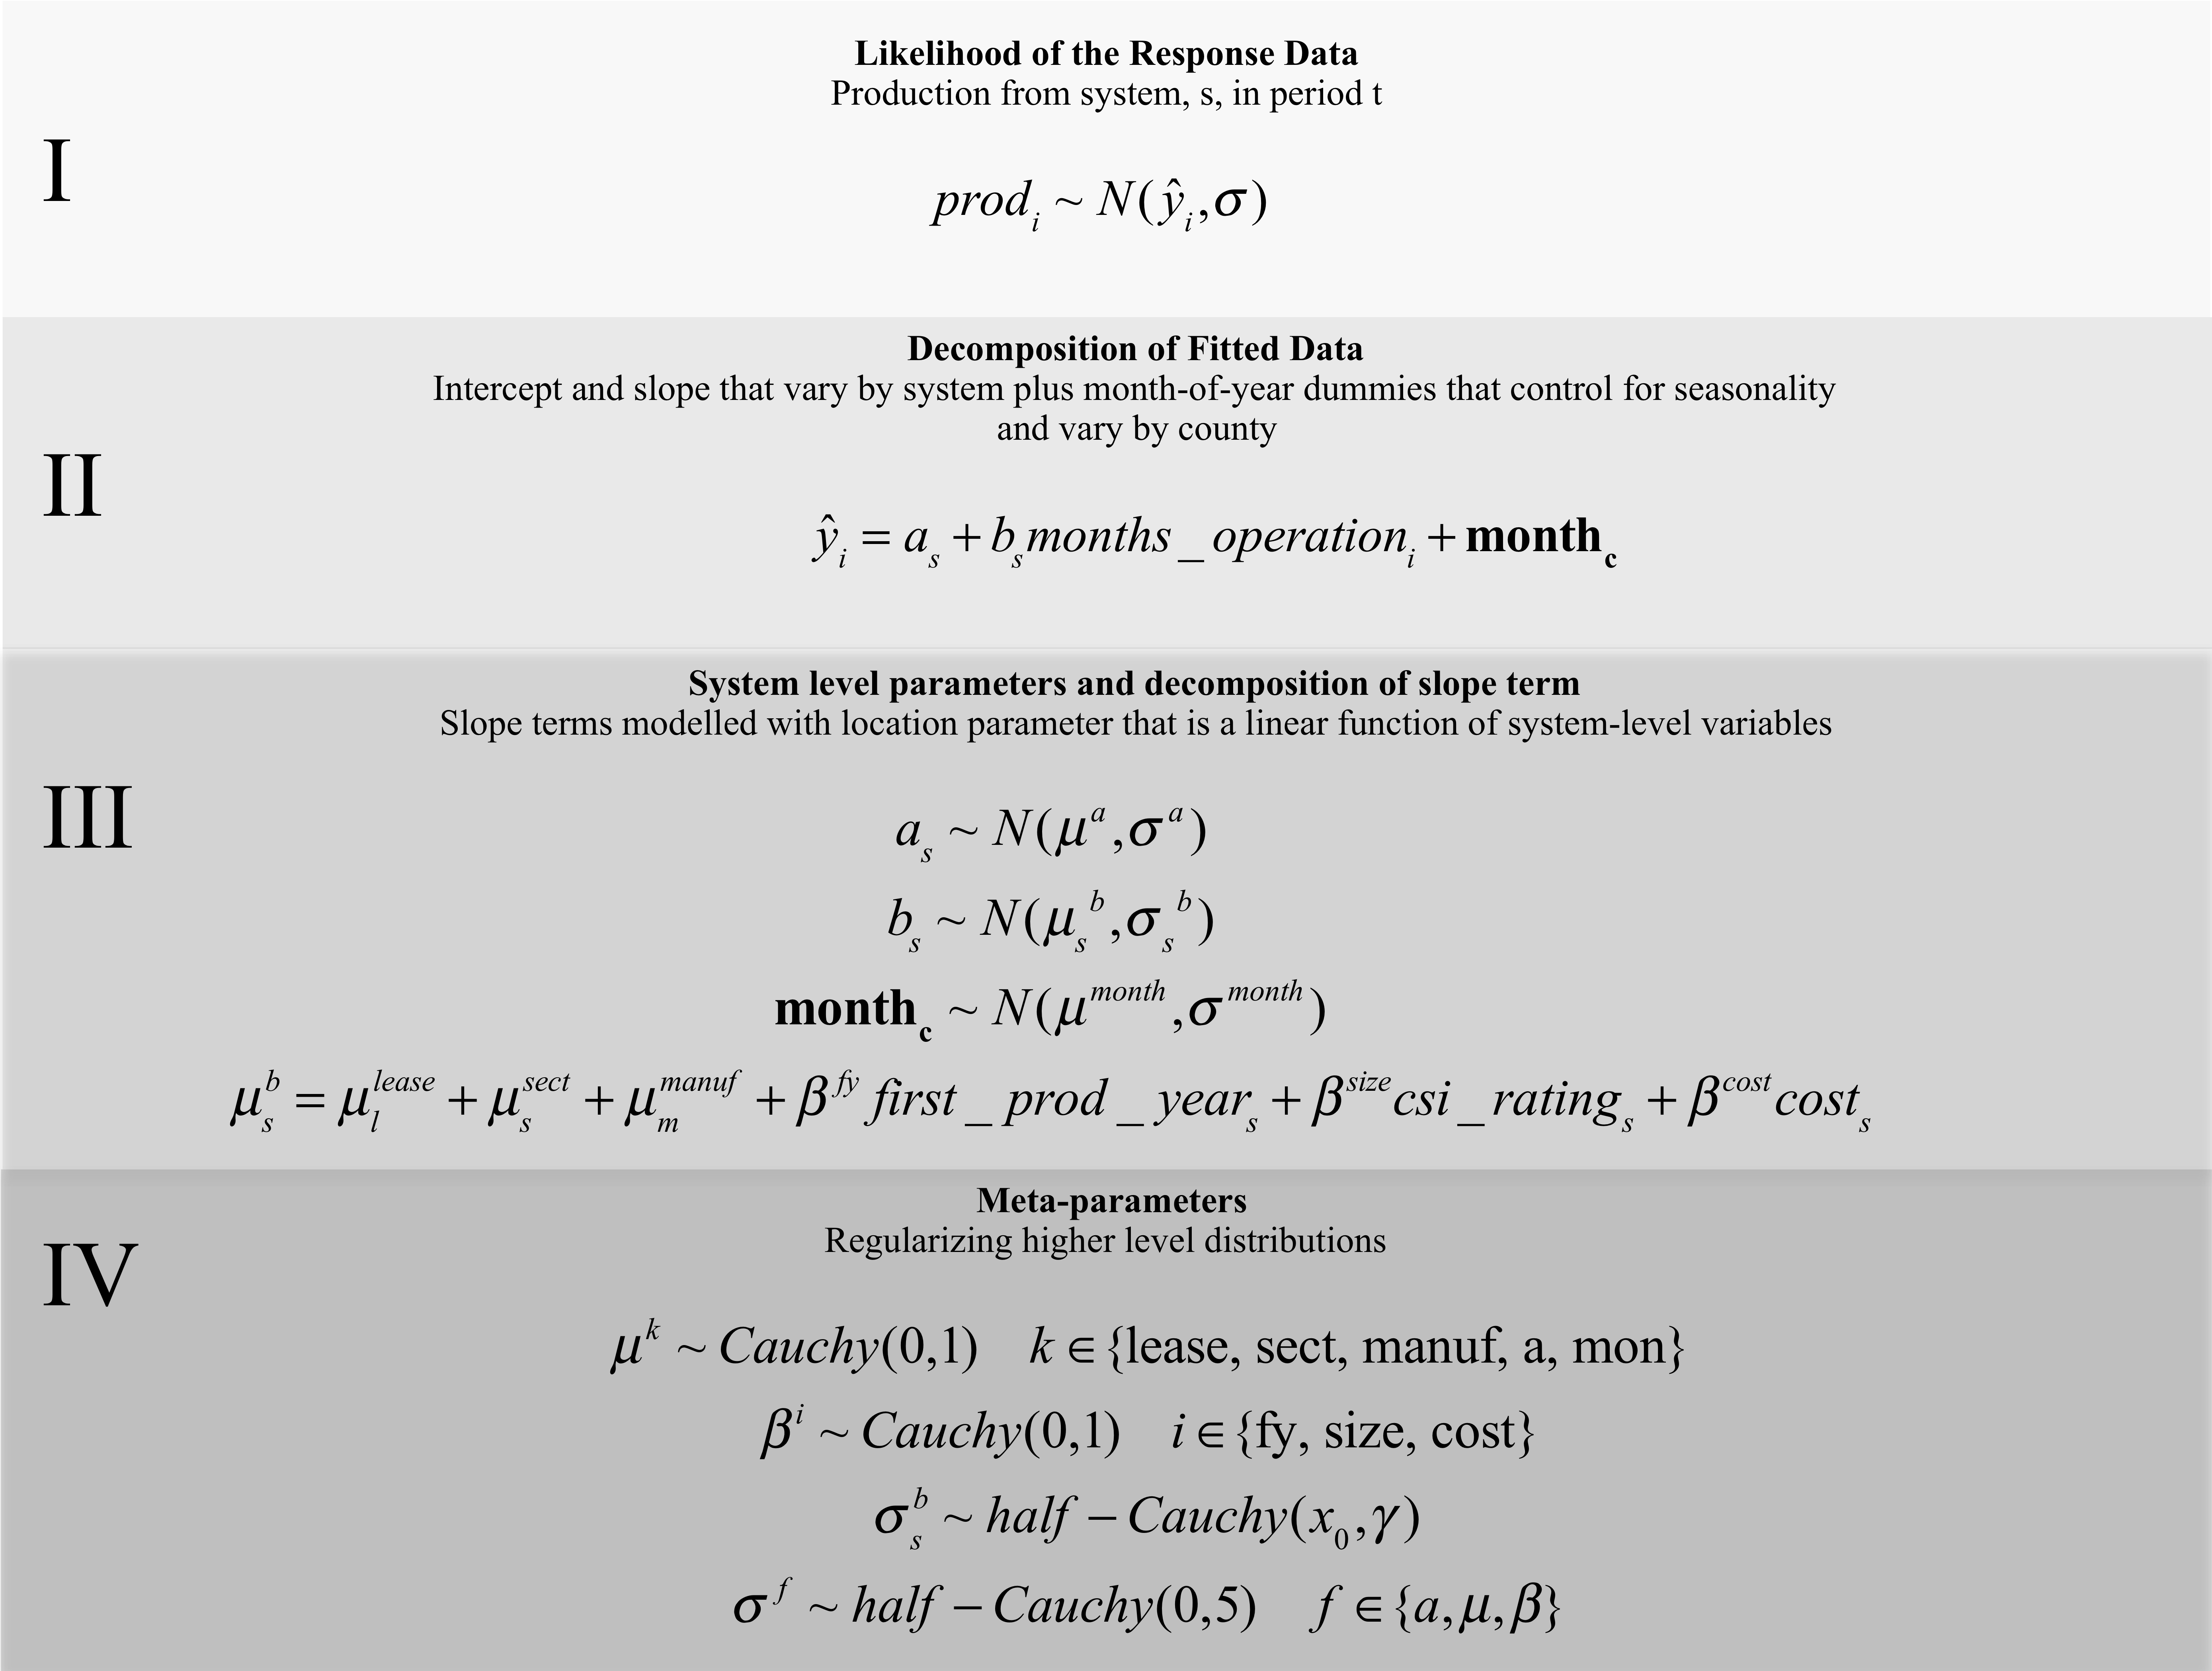
\includegraphics[width=1\textwidth]{figures/solar_prod_hierarchy.png}
	\caption{An overview of the structure of the model. Starting from the top in panel I, the monthly production data is modeled with a normally distributed likelihood. Moving down to II, the fitted values, $\hat{y}_{st}$, are in turn decomposed into system-varying slope and intercept terms, as well as month-dummies that control for seasonality. Further down to III, the slope terms, $b_s$ are modeled as normal distributions with varying mean parameters, $\mu_b^s$ that decompose further into terms representing variables of interest and control variables. Finally, in IV, all parameters are given higher-level meta-parameters that serve to regularize (or "shrink") the lower-level parameter estimates.}
	\label{solar_prod_hierarchy}
\end{figure}

In the earlier section, we noticed that some of the system slope parameters were estimated to be positive. There are intuitive and plausible reasons for observing higher average production some time after the initial installation. The placement of solar panels could have been optimized after the fact. Malfunctioning components could also have been replaced. However, when we wish to interpret the $b_s$ parameters as degradation over time, we should ideally discount positive values. Several possibilities present themselves. I could discard the systems with positive slope parameters from the data used. But discarding data and the associated information is generally not a desirable. Alternatively, I could keep in all data, allowing for the slope terms to be positive. After all, one of the advantages of the hierarchical model with weakly regularizing priors is that it allows for outlying parameter estimates, without unduly effecting the overall results. A third solution is to include all the data, but constrain the model by having priors that place zero probability on positive slope parameter values. $b_s$ parameters would be given half-Cauchy distributions with support between 0 and negative infinity. This has the desired effect of constraining slope parameters to be negative by imposing prior knowledge. The downside is that such strong priors can sometimes lead to unintended effects on the posterior distribution and can lead to faulty inference. In the proceeding analysis I therefor present results from both constrained and unconstrained models.

\subsection{Computation and Results from Bayesian hierarchical model}

The model is estimated using the Stan probabilistic programming language and sampler, which implements Hamiltonian MCMC and a No U-turn sampler (NUTS) \citep{stan_development_team_stan_2014}. The sampler was run with four chains and 1000 iterations. A Gelman-Rubin convergence statistic ($\hat{R}$ of 1 indicated convergence in the model. 2000 samples are taken from the simulated posterior distribution, and model results for the marginal distributions of the parameters of interest are presented in the form of kernel densities of the samples.

Recall that the testable implications from the theory of asymmetric information and quality were that 1.) average quality should be higher in the panels owned by the high-information type (leased panels). 2.) Price should be more highly correlated with quality in the panels owned by the high-information type.

The parameters of interest in our model are then the higher level parameters $\mu_l^{lease}$ and $\beta_l$. The first represents the mean value of the system level slope terms, $b_s$ grouped by whether the systems were leased or host-owned. The latter is a measure of the correlation between the cost of the system and the system slope terms. The $\beta_l$ parameter is also allowed to vary by leased or host-owned. It is important to note, that the estimated $\beta_l$ parameters are estimated conditional on the installation date of the solar panels, thus they do not reflect changes in price over time. This could lead to a heavy bias in the results if, as seems plausible, both prices and quality changed over time.

For the testable implications, the inference we are interested is in the contrasts, $\mu_{lease, yes} - \mu_{lease, no}$ and $\beta_{leased}- \beta_{owned}$. Kernel densities representing the marginal distributions of these contrasts are presented in figure \ref{fig:contrasts}. The top panel shows the distribution of the contrast $\mu_{lease, yes} - \mu_{lease, no}$. Essentially all of the probability mass is located in the positive range. This reinforces the finding from the mixed effects model that leased panels do appear to have substantially higher quality, as the theory of asymmetric information of quality would suggest.

The evidence for the second testable implication is less conclusive. The model estimates that there is approximately a 89\% probability that there is a higher correlation between quality and cost for the high information type owner of leased panels compared to the low information type owner of host-owned panels.

Figure \ref{fig:contrasts_const} show the corresponding distributions under the constrained model. $\mu_{lease, yes} - \mu_{lease, no}$ is pulled somewhat towards zero in magnitude, but nearly all of the probability mass is still in the positive range. The distribution of  $\beta_{leased}- \beta_{owned}$ is also pulled towards zero, and now 72\% of the probability mass is in the positive range.

\begin{figure}
\begin{minipage}{.48\textwidth}
  \centering
  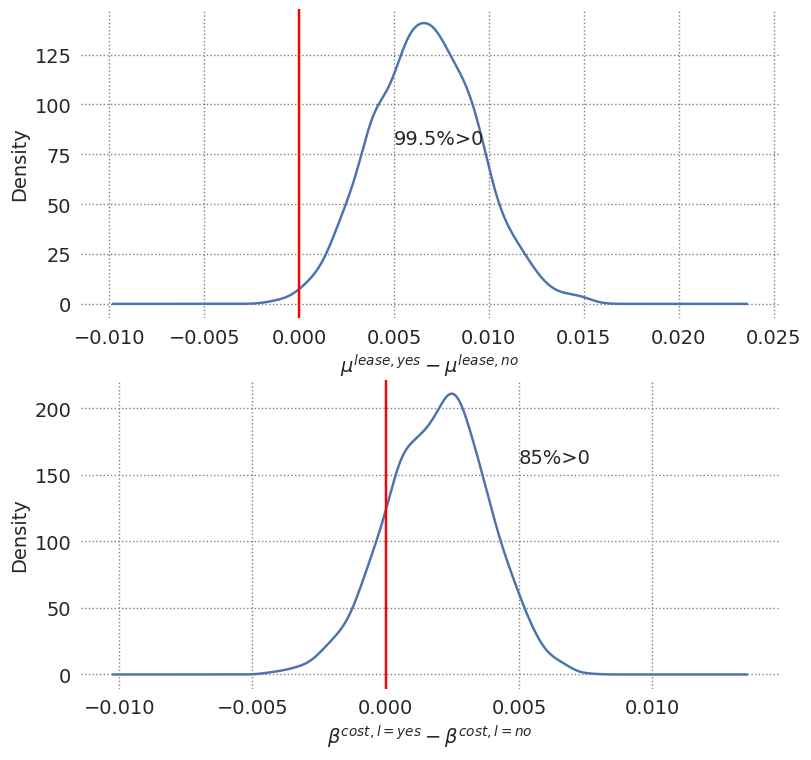
\includegraphics[width=1\linewidth]{figures/bayes_hypos.png}
  \label{fig:contrasts}
 \end{minipage}\qquad
\begin{minipage}{.48\textwidth}
  \centering
  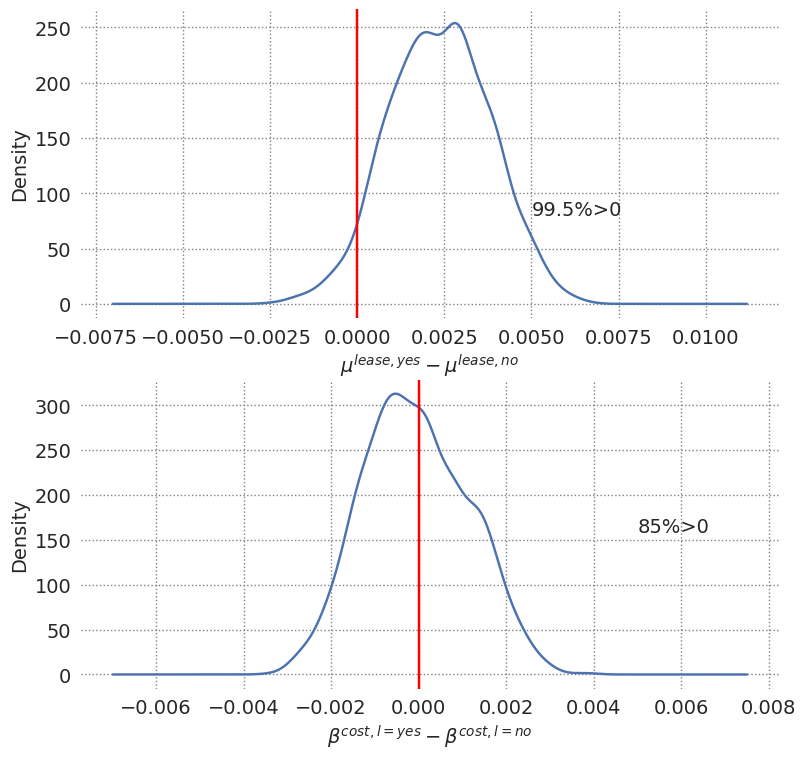
\includegraphics[width=1\linewidth]{figures/bayes_hypos_const.png}
  \label{fig:contrasts_const}
 \end{minipage}
\bigskip
\begin{minipage}[t]{.48\textwidth}
\centering
\caption{Marginal posterior distributions for the contrasts of interest. The top panel shows that the distributions of the slope parameters, $b_s$, are estimated to have means that are significantly different from each other between leased and host-owned systems as defined by the contrast, $\mu_{lease, yes} - \mu_{lease, no}$. The lower panel shows the marginal posterior distribution of the contrast between the $\beta$ parameter for leased and host-owned solar systems. The results indicate that there is an approximately 89\% probability that costs are more highly correlated with quality in leased systems compared to those that are host-owned.}
\end{minipage}\qquad
\begin{minipage}[t]{.48\textwidth}
\centering
 \caption{Marginal posterior distributions for the contrasts when the $b_s$ paramaters and corresponding higher-level mean parameters are constrained to have a maximum of zero. The contrast, $\mu_{lease, yes} - \mu_{lease, no}$ is materially unchanged and continues to have nearly its entire distribution in a positive range, though it is pulled somewhat towards zero. The contrast $\beta_{lease, yes} - \beta_{lease, no}$ is also pulled towards zero, and now only approximately 72 \% of the probability is in a positive range. The results indicate that there is an approximately 72\% probability that costs are more highly correlated with quality in leased systems compared to those that are host-owned when all higher level mean parameters are constrained to have a maximum of zero.}
\end{minipage}
\end{figure}

A direct comparison of costs between leased and host-owned solar power systems is somewhat complicated. The prices of host-owned panels are market prices: simply the purchase price that the owner of the solar panel system paid to the contractor. On the other hand, the price of leased systems is a reported price from the contractors consisting of the component and installation costs plus an estimated mark-up. If these costs were reported correctly, then the theory should still hold. The reported cost should reflect the ability of the high-information owners to judge quality of the panels that they purchase. In practice, the reliability of reported cost is a source of added uncertainty, and should be taken into consideration when interpreting the results.

However, if we assume that misreporting of the true costs will tend to lead to less variation in reported costs, then that should have the effect of attenuating the magnitude of the contrast, $\beta_{cost, l=yes} - \beta_{cost, l=no}$. In that case, the estimated contrast can be seen as being a conservative estimate.

Summary statistics of the distributions of higher level parameters are reported in table \ref{table:higher_level_params} and table \ref{table:higher_level_params_const} for the constrained model. The sector groupings, $\mu^{sect}$ can be of interest in a discussion of the role of asymmetric information. Figure \ref{fig:mu_sectors} shows the distributions of the contrasts relative to the residential host sector. The top panel represents the contrast with commercial sector hosts, the middle with government sector host and the bottom panel with non-profit sector host. All three contrasts indicate relatively lower quality for installations for these sectors compared to the residential sector. Results of the constrained model are shown in figure \ref{fig:mu_sectors_const}. The results are similar, though the difference in average quality between the government and residential sector is now centered closely around zero.

While it is not clear why this should be, an explanation consistent with the theory of asymmetric information of quality is that there exists an agency problem. A homeowner will, in some form, have a direct financial incentive to acquire solar panels of good quality. On the other hand, A manager or employee of a firm, government agency or non-profit may not have any direct financial incentive in ensuring that a solar panel system is of high quality.

\begin{table}
  \begin{tabular}{lrrrrrrrrr}
  \toprule
  {} &    mean &    std &     min &    2.5\% &     25\% &     50\% &     75\% &   97.5\% &     max \\
  \midrule
  $\mu^{meta}$     &  0.004' & 0.022' & -0.018' & -0.010' & -0.007' & -0.005' & -0.002' &  0.069' &  0.084' \\
  $\beta^{meta}$   &  0.003' & 0.838' & -8.120' & -1.707' & -0.074' & -0.007' &  0.075' &  1.738' &  6.787' \\
  $\mu^{meta,mon}$ &  0.005' & 0.036' & -0.138' & -0.065' & -0.019' &  0.006' &  0.030' &  0.075' &  0.146' \\
  $\mu^{b_s}$      & -0.000' & 0.015' & -0.043' & -0.028' & -0.012' & -0.002' &  0.011' &  0.031' &  0.044' \\
  $\mu^{jan}$      & -0.164' & 0.013' & -0.188' & -0.186' & -0.173' & -0.163' & -0.154' & -0.144' & -0.142' \\
  $\mu^{feb}$      & -0.121' & 0.013' & -0.146' & -0.143' & -0.131' & -0.120' & -0.111' & -0.102' & -0.100' \\
  $\mu^{mar}$      & -0.054' & 0.013' & -0.078' & -0.076' & -0.064' & -0.053' & -0.044' & -0.035' & -0.033' \\
  $\mu^{apr}$     &  0.040' & 0.013' &  0.017' &  0.018' &  0.031' &  0.042' &  0.051' &  0.060' &  0.062' \\
  $\mu^{may}$      &  0.087' & 0.013' &  0.063' &  0.064' &  0.077' &  0.088' &  0.097' &  0.106' &  0.108' \\
  $\mu^{jun}$      &  0.111' & 0.013' &  0.087' &  0.089' &  0.102' &  0.113' &  0.121' &  0.131' &  0.133' \\
  $\mu^{jul}$      &  0.108' & 0.013' &  0.084' &  0.086' &  0.099' &  0.110' &  0.118' &  0.128' &  0.130' \\
  $\mu^{aug}$      &  0.101' & 0.013' &  0.077' &  0.079' &  0.092' &  0.103' &  0.112' &  0.121' &  0.123' \\
  $\mu^{sep}$     &  0.082' & 0.013' &  0.058' &  0.060' &  0.072' &  0.083' &  0.092' &  0.102' &  0.103' \\
  $\mu^{oct}$      &  0.026' & 0.013' &  0.002' &  0.004' &  0.016' &  0.027' &  0.036' &  0.045' &  0.047' \\
  $\mu^{nov}$     & -0.031' & 0.013' & -0.056' & -0.053' & -0.041' & -0.030' & -0.021' & -0.011' & -0.010' \\
  $\mu^{dec}$     & -0.123' & 0.013' & -0.147' & -0.146' & -0.133' & -0.122' & -0.113' & -0.104' & -0.101' \\
  $\mu^{lease, no}$   & -0.030' & 0.045' & -0.193' & -0.159' & -0.015' & -0.011' & -0.008' & -0.002' &  0.015' \\
  $\mu^{lease, yes}$   & -0.022' & 0.045' & -0.186' & -0.151' & -0.007' & -0.003' &  0.000' &  0.006' &  0.023' \\
  $\mu^{sect, com}$      &  0.002' & 0.022' & -0.024' & -0.015' & -0.010' & -0.007' & -0.004' &  0.066' &  0.087' \\
  $\mu^{sect, res}$       &  0.012' & 0.022' & -0.014' & -0.005' & -0.000' &  0.003' &  0.006' &  0.075' &  0.096' \\
  $\mu^{sect, gov}$       &  0.006' & 0.022' & -0.017' & -0.010' & -0.005' & -0.003' &  0.001' &  0.071' &  0.092' \\
  $\mu^{sect, npr}$      & -0.001' & 0.022' & -0.026' & -0.018' & -0.012' & -0.010' & -0.006' &  0.063' &  0.084' \\
  $\beta^{cost, l=no}$  & -0.002' & 0.002' & -0.007' & -0.005' & -0.003' & -0.002' & -0.001' &  0.001' &  0.004' \\
  $\beta^{cost, l=yes}$  &  0.001' & 0.001' & -0.002' & -0.001' &  0.000' &  0.001' &  0.001' &  0.002' &  0.003' \\
  $\beta^{size}$  &  0.002' & 0.001' & -0.001' &  0.000' &  0.002' &  0.002' &  0.003' &  0.004' &  0.006' \\
  $\beta^{fy}$    & -0.018' & 0.001' & -0.021' & -0.020' & -0.018' & -0.018' & -0.017' & -0.016' & -0.014' \\
  $\sigma$      &  0.065' & 0.000' &  0.065' &  0.065' &  0.065' &  0.065' &  0.065' &  0.066' &  0.066' \\
  $\sigma^{b_s}$    &  0.476' & 0.006' &  0.454' &  0.465' &  0.472' &  0.476' &  0.480' &  0.488' &  0.495' \\
  $\sigma^{mon}$   &  0.114' & 0.030' &  0.059' &  0.074' &  0.094' &  0.108' &  0.128' &  0.185' &  0.341' \\
  $\sigma^{\beta}$  &  0.833' & 1.773' &  0.001' &  0.006' &  0.047' &  0.195' &  0.836' &  5.675' & 19.879' \\
  $\sigma^{mu}$   &  0.006' & 0.001' &  0.003' &  0.004' &  0.005' &  0.006' &  0.006' &  0.008' &  0.011' \\
  \bottomrule
  \end{tabular}
\label{table:higher_level_params}
\caption{Summary statistics of the estimated posterior distributions of higher level parameters}
\end{table}

% constrained table

\begin{table}
\begin{tabular}{lrrrrrrrrr}
\toprule
{} &    mean &    std &     min &    2.5\% &     25\% &     50\% &     75\% &   97.5\% &           max \\
\midrule
beta1\_fy0    & -0.017' & 0.001' & -0.021' & -0.019' & -0.018' & -0.017' & -0.017' & -0.016' & -1.454096e-02 \\
meta\_mu0     & -0.006' & 0.001' & -0.009' & -0.008' & -0.007' & -0.006' & -0.006' & -0.005' & -3.700574e-03 \\
meta\_beta0   &  0.012' & 0.798' & -4.910' & -1.877' & -0.083' & -0.009' &  0.080' &  1.989' &  6.342196e+00 \\
meta\_mu\_mon0 & -0.114' & 0.034' & -0.280' & -0.180' & -0.137' & -0.115' & -0.093' & -0.044' &  3.362246e-02 \\
sigma\_mu10   &  0.003' & 0.001' &  0.002' &  0.002' &  0.003' &  0.003' &  0.003' &  0.004' &  5.319401e-03 \\
mu\_b00       &  0.121' & 0.011' &  0.088' &  0.101' &  0.113' &  0.121' &  0.129' &  0.142' &  1.531909e-01 \\
sigma\_b00    &  0.476' & 0.006' &  0.459' &  0.464' &  0.472' &  0.476' &  0.480' &  0.487' &  4.995173e-01 \\
sigma\_mon0   &  0.114' & 0.029' &  0.055' &  0.075' &  0.094' &  0.108' &  0.127' &  0.188' &  2.955012e-01 \\
sigma\_beta0  &  0.800' & 1.495' &  0.006' &  0.010' &  0.051' &  0.201' &  0.814' &  5.056' &  1.976847e+01 \\
sigma0       &  0.065' & 0.000' &  0.065' &  0.065' &  0.065' &  0.065' &  0.065' &  0.065' &  6.572528e-02 \\
mu\_mon0      & -0.285' & 0.007' & -0.298' & -0.297' & -0.290' & -0.286' & -0.278' & -0.275' & -2.736025e-01 \\
mu\_mon1      & -0.243' & 0.007' & -0.256' & -0.254' & -0.248' & -0.243' & -0.235' & -0.233' & -2.310124e-01 \\
mu\_mon2      & -0.176' & 0.007' & -0.189' & -0.187' & -0.181' & -0.176' & -0.168' & -0.166' & -1.642462e-01 \\
mu\_mon3      & -0.081' & 0.007' & -0.094' & -0.093' & -0.086' & -0.082' & -0.074' & -0.071' & -6.978557e-02 \\
mu\_mon4      & -0.035' & 0.007' & -0.048' & -0.047' & -0.040' & -0.035' & -0.028' & -0.025' & -2.350794e-02 \\
mu\_mon5      & -0.010' & 0.007' & -0.023' & -0.022' & -0.015' & -0.011' & -0.003' & -0.000' & -1.024029e-05 \\
mu\_mon6      & -0.013' & 0.007' & -0.026' & -0.025' & -0.018' & -0.014' & -0.006' & -0.003' & -1.735978e-03 \\
mu\_mon7      & -0.020' & 0.007' & -0.034' & -0.031' & -0.025' & -0.021' & -0.013' & -0.010' & -8.326959e-03 \\
mu\_mon8      & -0.039' & 0.007' & -0.053' & -0.051' & -0.045' & -0.040' & -0.032' & -0.030' & -2.838155e-02 \\
mu\_mon9      & -0.096' & 0.007' & -0.109' & -0.107' & -0.101' & -0.096' & -0.089' & -0.086' & -8.434625e-02 \\
mu\_mon10     & -0.152' & 0.007' & -0.166' & -0.164' & -0.158' & -0.153' & -0.145' & -0.143' & -1.412385e-01 \\
mu\_mon11     & -0.245' & 0.007' & -0.258' & -0.256' & -0.250' & -0.245' & -0.237' & -0.235' & -2.336429e-01 \\
mu1\_lease0   & -0.005' & 0.001' & -0.008' & -0.007' & -0.006' & -0.005' & -0.005' & -0.004' & -2.602403e-03 \\
mu1\_lease1   & -0.000' & 0.000' & -0.002' & -0.001' & -0.000' & -0.000' & -0.000' & -0.000' & -5.518242e-08 \\
mu1\_s0       & -0.002' & 0.001' & -0.005' & -0.004' & -0.003' & -0.002' & -0.002' & -0.001' & -1.790787e-04 \\
mu1\_s1       & -0.001' & 0.000' & -0.003' & -0.002' & -0.001' & -0.000' & -0.000' & -0.000' & -2.355766e-06 \\
mu1\_s2       & -0.001' & 0.001' & -0.004' & -0.002' & -0.001' & -0.001' & -0.000' & -0.000' & -1.807113e-06 \\
mu1\_s3       & -0.007' & 0.002' & -0.014' & -0.010' & -0.008' & -0.007' & -0.006' & -0.004' & -2.390480e-03 \\
beta1\_cost0  & -0.000' & 0.002' & -0.005' & -0.003' & -0.001' & -0.000' &  0.001' &  0.003' &  4.742583e-03 \\
beta1\_cost1  &  0.001' & 0.001' & -0.002' & -0.001' &  0.000' &  0.001' &  0.001' &  0.002' &  3.464386e-03 \\
beta1\_size0  &  0.001' & 0.001' & -0.002' & -0.000' &  0.001' &  0.001' &  0.002' &  0.003' &  3.930082e-03 \\
\bottomrule
\end{tabular}
\label{table:higher_level_params_const}
\caption{Summary statistics of the estimated posterior distributions of higher level parameters when higher level mean parameters are constrained to have a maximum of zero.}
\end{table}


%\begin{figure}
%  \centering
%  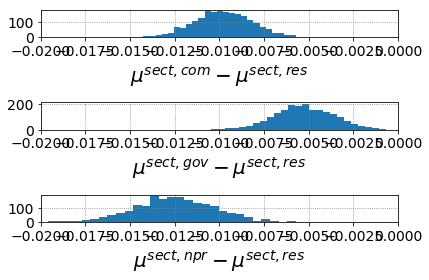
\includegraphics[width=1\linewidth]{figures/mu_sectors.png}
%  \caption{Distribution of the sector contrasts relative to residential sector. Installations for commercial, governmental and non-profit hosts are shown to have on average lower quality then installations in residential}
%  \label{mu_sectors}
%\end{figure}


\begin{figure} [!htb]
\begin{minipage}{.48\textwidth}
  \centering
  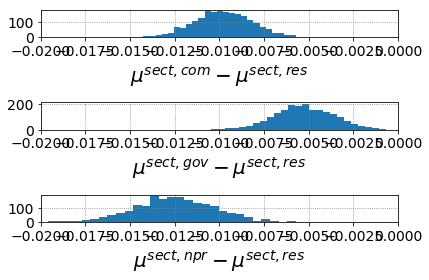
\includegraphics[width=1\linewidth]{figures/mu_sectors.png}
  \label{fig:mu_sectors}
 \end{minipage}\qquad
\begin{minipage}{.48\textwidth}
  \centering
  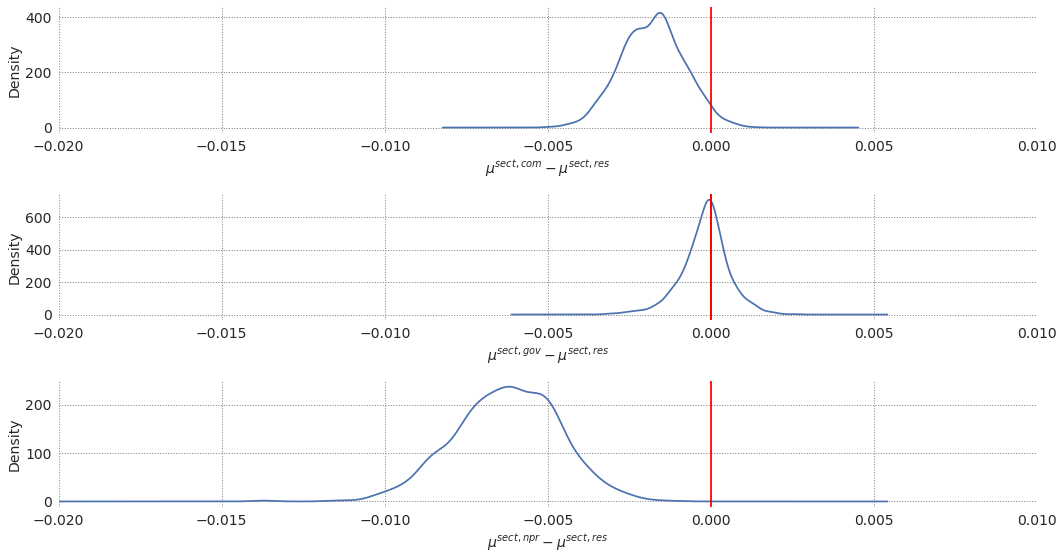
\includegraphics[width=1\linewidth]{figures/mu_sectors_const.png}
  \label{fig:mu_sectors_const}
 \end{minipage}

\bigskip

\begin{minipage}[t]{.48\textwidth}
\centering
 \caption{Distribution of the sector contrasts relative to residential sector. Installations for commercial, governmental and non-profit hosts are shown to have on average lower quality then installations in residential}
\end{minipage}\qquad
\begin{minipage}[t]{.48\textwidth}
\centering
 \caption{Distribution of the sector contrasts relative to residential sector when all higher level mean parameters are constrained to have a maximum of zero. Installations for commercial, governmental and non-profit hosts are shown to have on average lower quality then installations in residential}
\end{minipage}
\end{figure}

Summary statistics for the parameters on the manufacturer group means as well as the lower-level intercept and slope parameters $a_s$ and $b_s$ are too numerous to present in a table. Visual summaries are presented in figures \ref{fig:BayManPlot}, \ref{fig:Bay_as} and \ref{fig:Bay_bs}. Figure \ref{fig:BayManPlot} shows box plots of the manufacturer distributions, with the box representing 70 percent of probability and the lines representing 95 percent of the probability. Mirroring earlier results, the plot shows most manufacturers with roughly equivalent quality, with a handful with meaningfully lower quality. Figures \ref{fig:Bay_as} and \ref{fig:Bay_bs} show 95\% intervals of the distribution of the $a_s$ and $b_s$ parameters. The intercept terms are shown to have considerable variation between systems, as would be expected, but are individually estimated precisely.

The slope parameters, $b_s$ are modeled explicitly and are also allowed to have varying variance parameters. This is evident in the plot. A similar pattern to the higher-level manufacturer group means is apparent: modest differences in quality are seen between most systems, with the exception of a lower tail of systems with particularly poor quality.

\begin{figure}
\begin{minipage}{.45\textwidth}
  \centering
  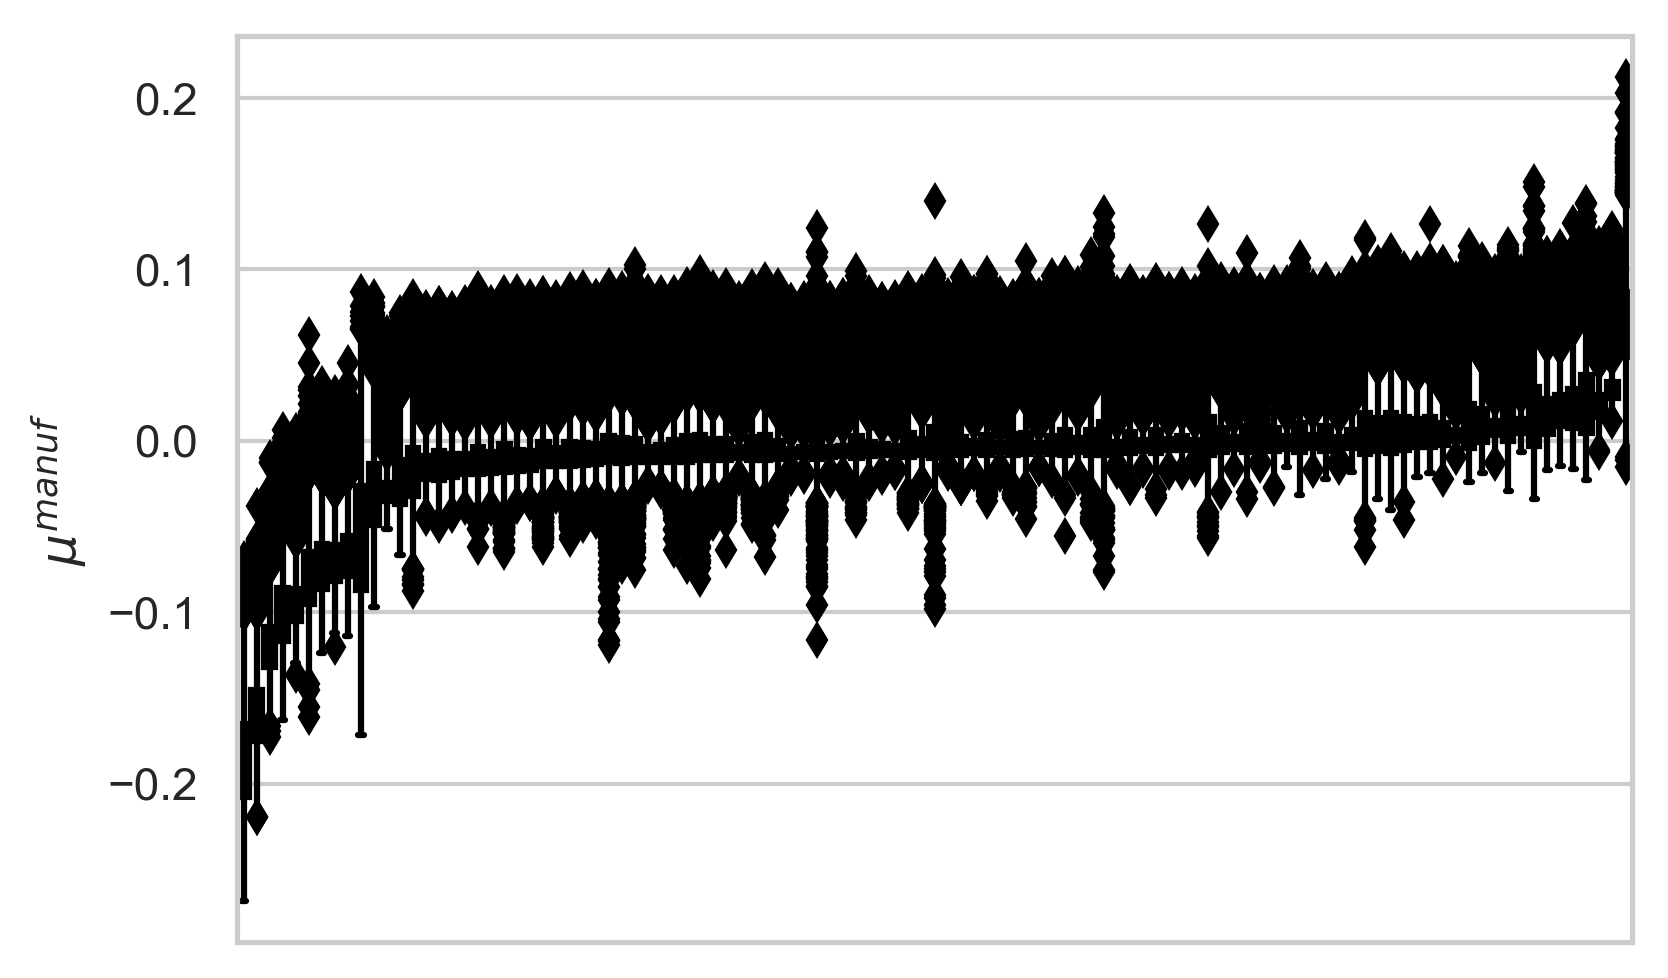
\includegraphics[width=1\linewidth]{figures/BayManPlot.png}
  \label{fig:BayManPlot}
 \end{minipage}\qquad
\begin{minipage}{.45\textwidth}
  \centering
  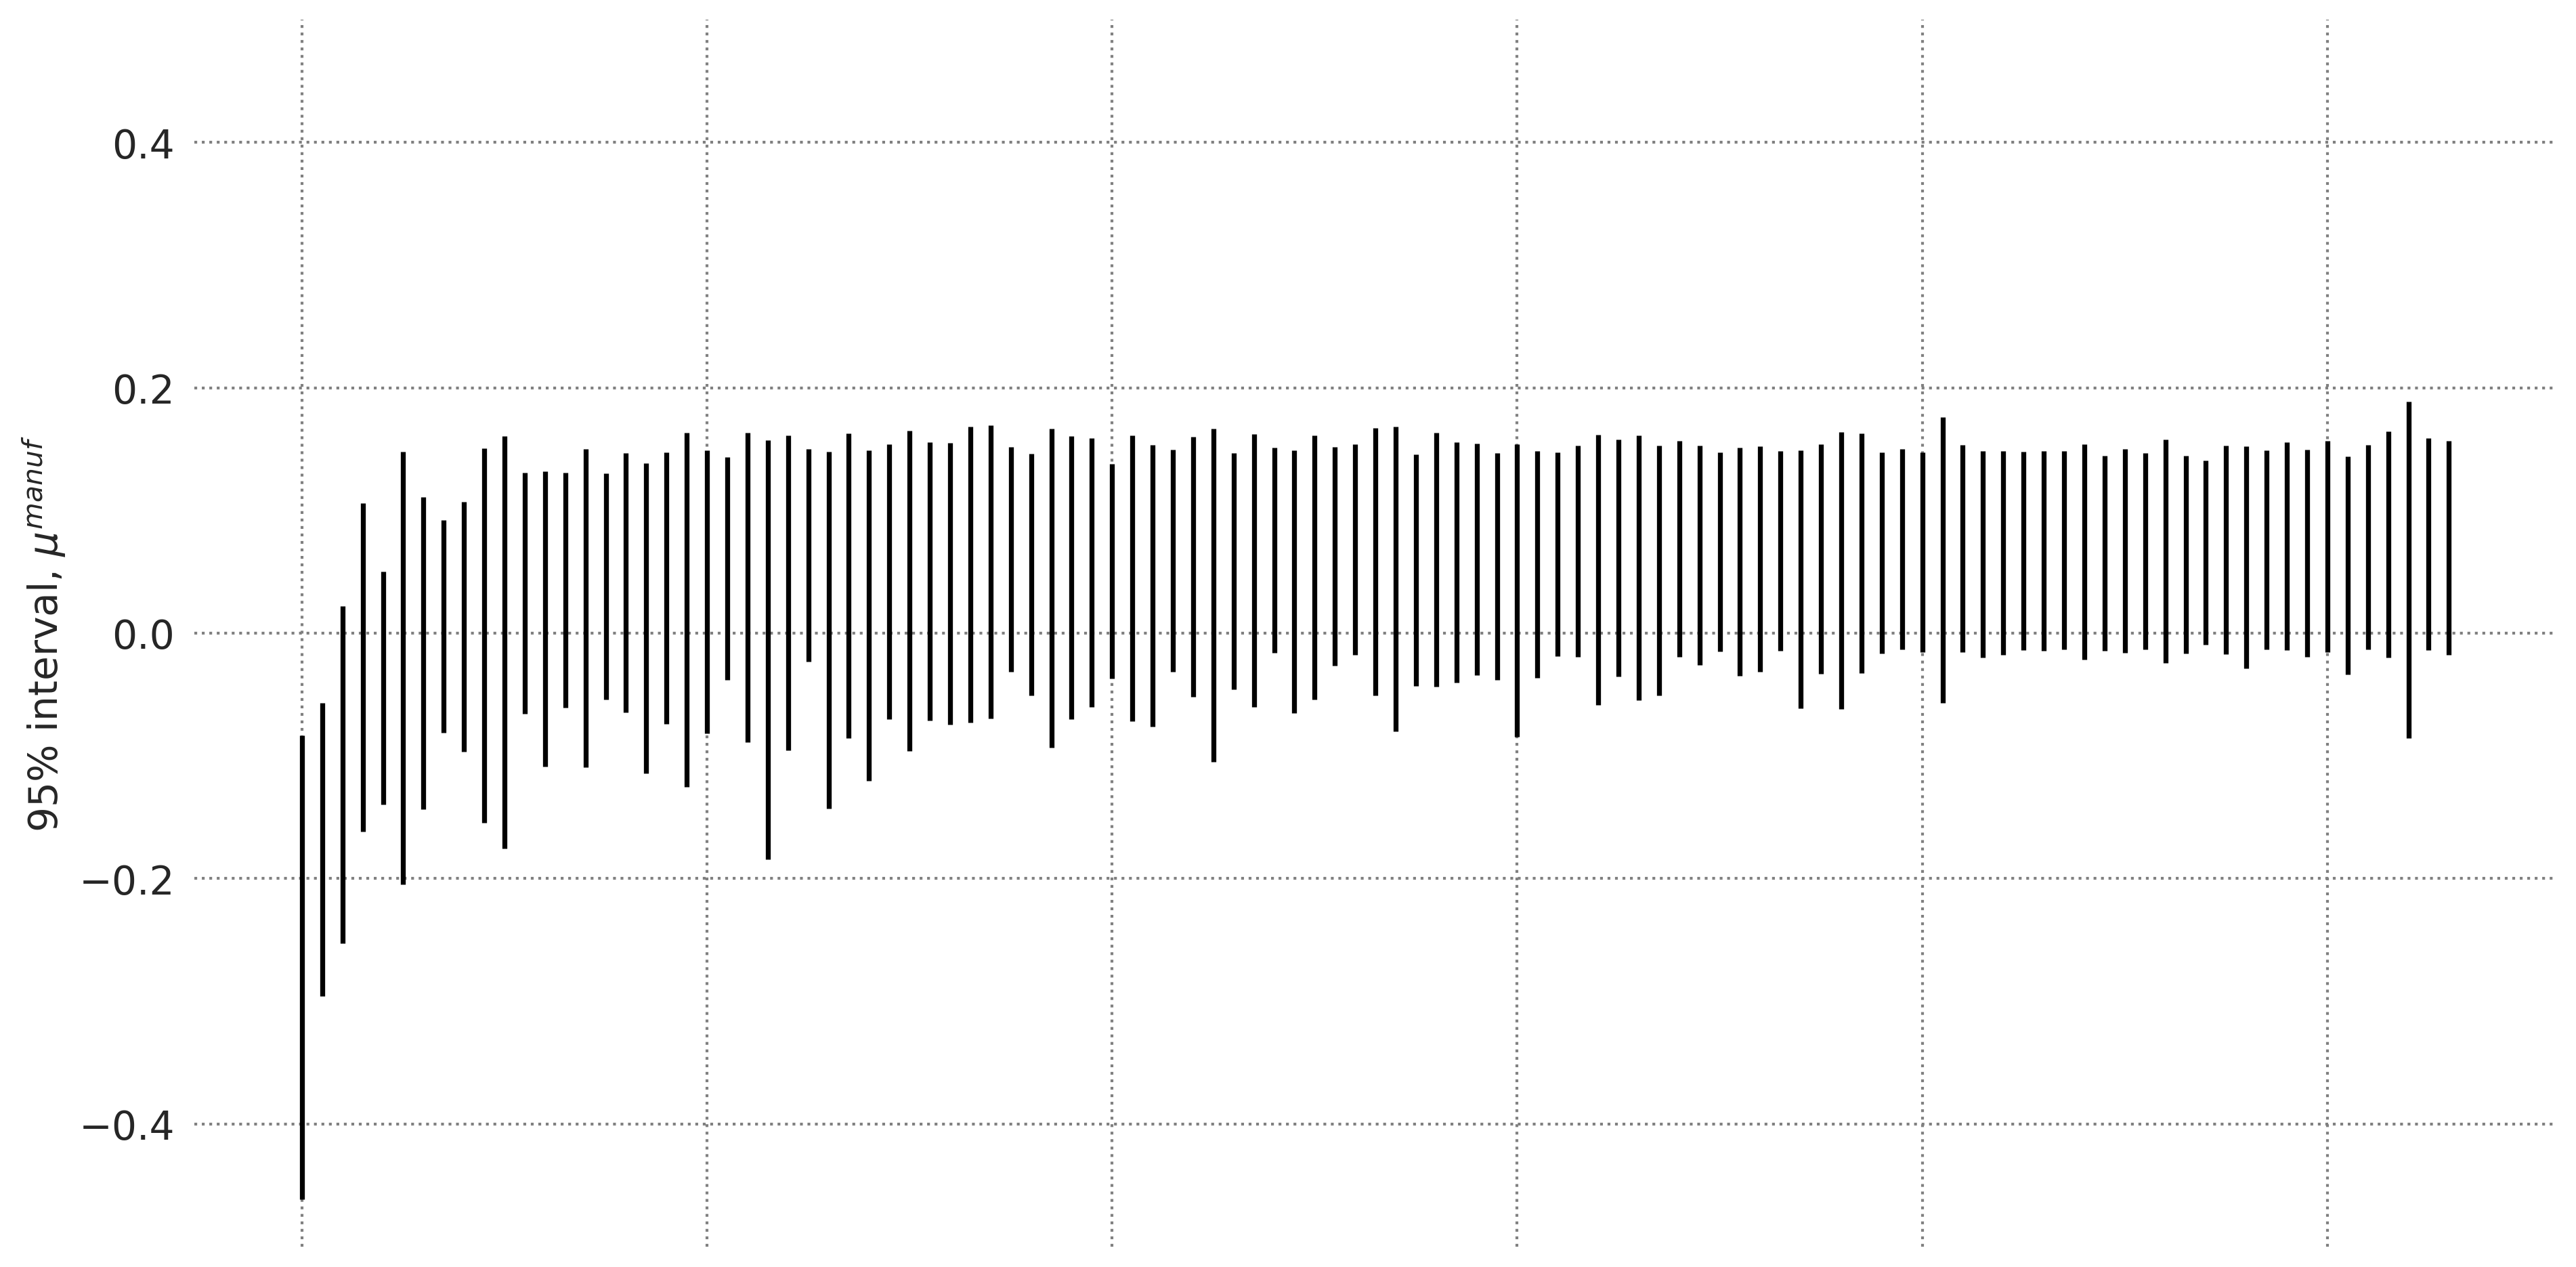
\includegraphics[width=1\linewidth]{figures/BayManPlot_const.png}
  \label{fig:BayManPlot_const}
 \end{minipage}

\bigskip

\begin{minipage}[t]{.45\textwidth}
\centering
  \caption{Box plot of the the parameters $\mu^{manuf}$, representing the distributions of the mean parameter for manufacturer groupings.}
\end{minipage}\qquad
\begin{minipage}[t]{.45\textwidth}
\centering
  \caption{Box plot of the the parameters $\mu^{manuf}$, when all higher level mean parameters have a maximum of zero.}
\end{minipage}
\end{figure}


%new image


\begin{figure}
\begin{minipage}{.45\textwidth}
  \centering
  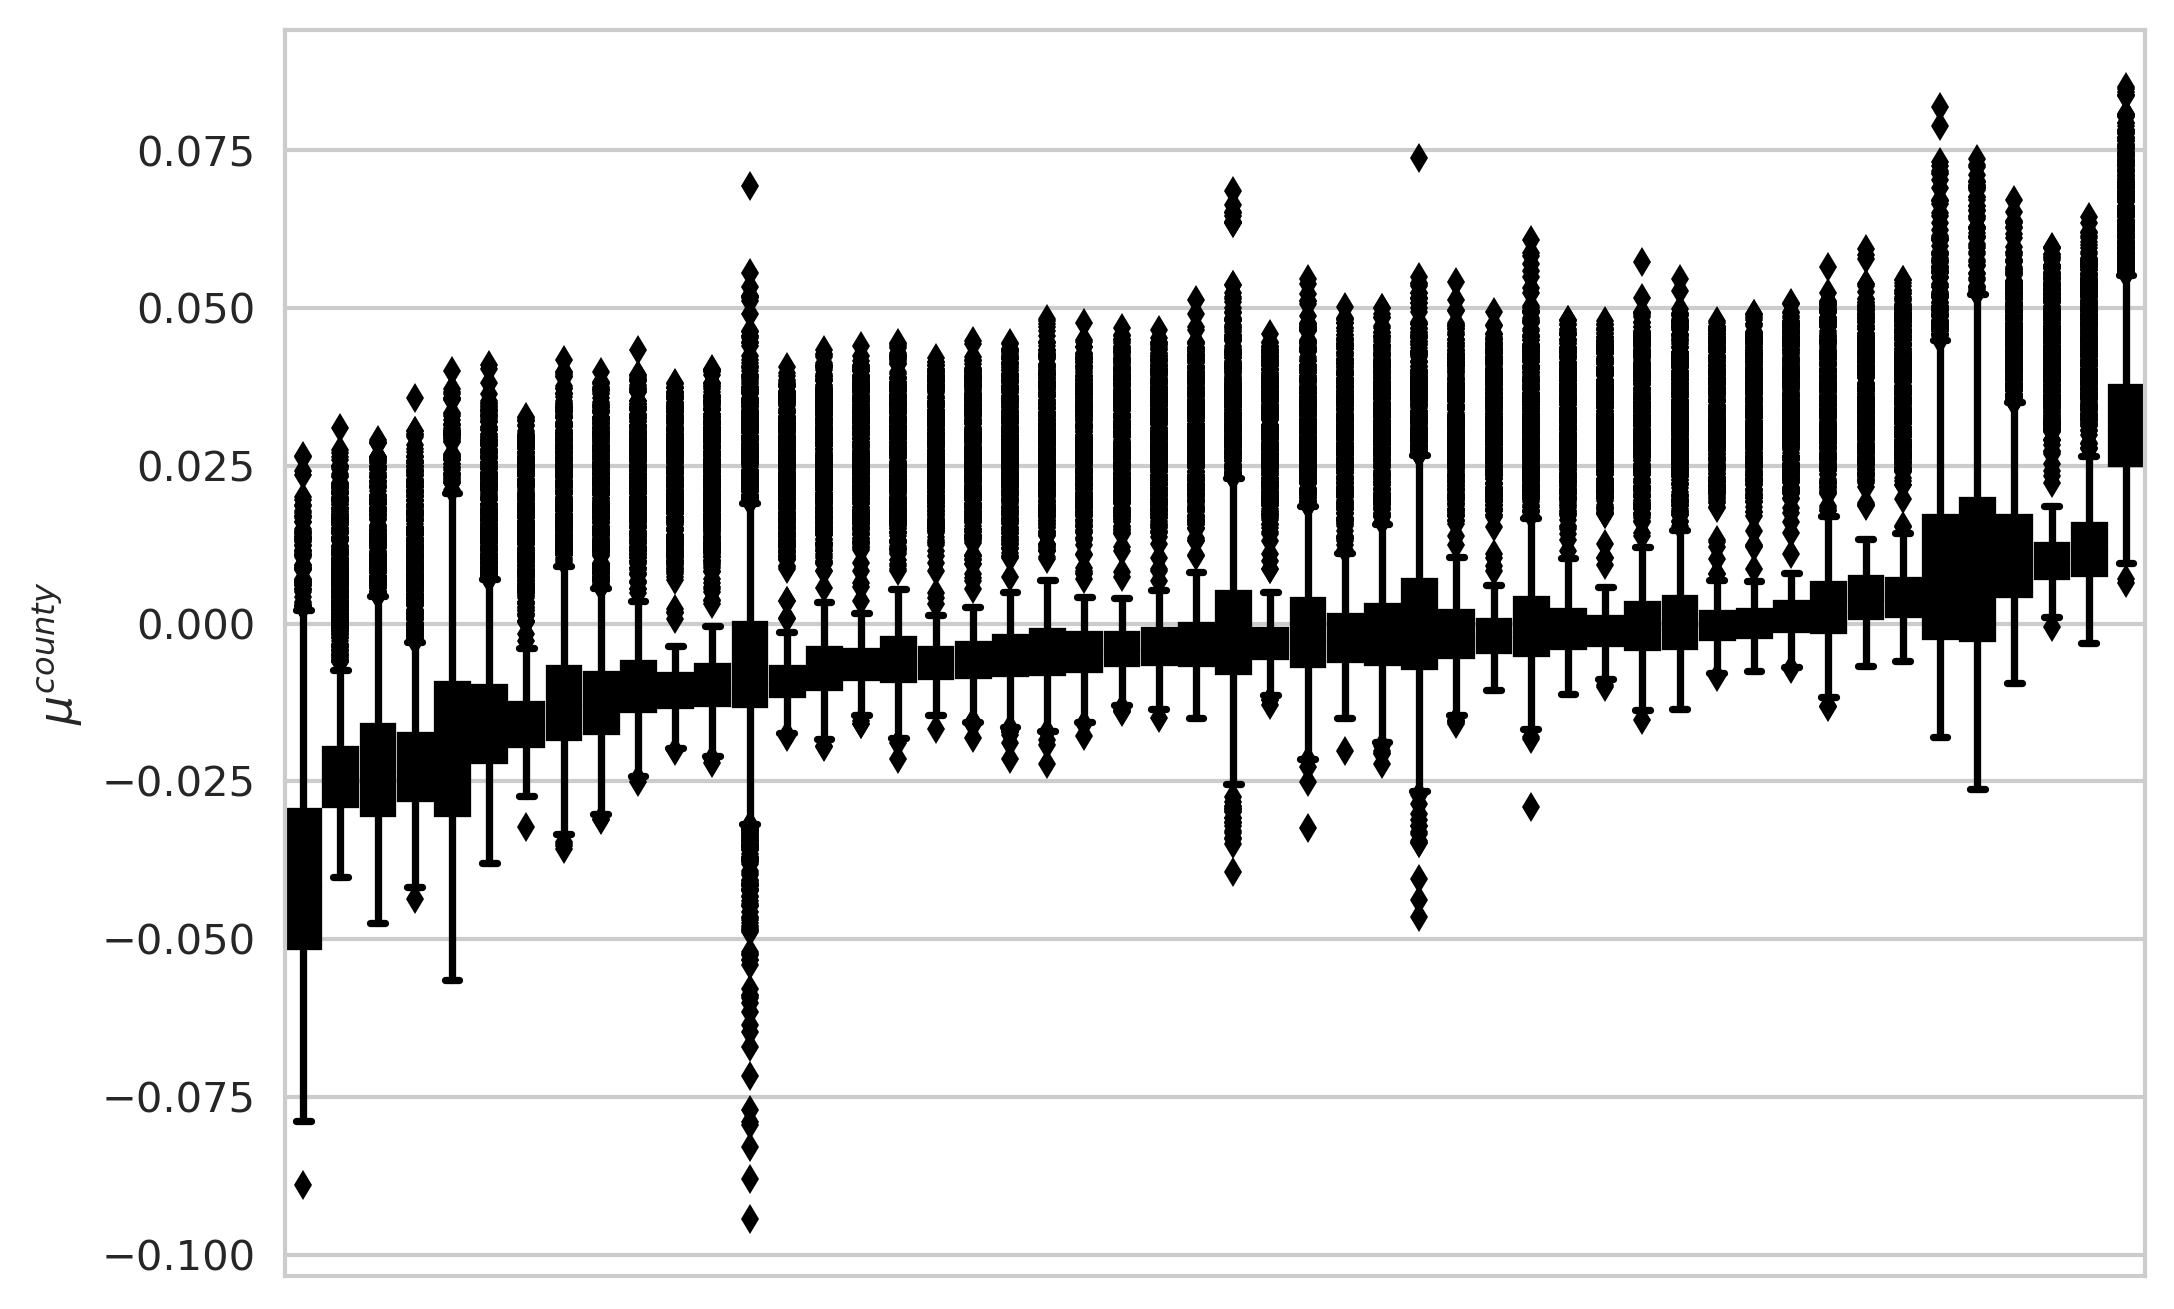
\includegraphics[width=1\linewidth]{figures/BayCountyPlot.png}
	\label{fig:BayCountyPlot}
 \end{minipage}\qquad
\begin{minipage}{.45\textwidth}
  \centering
  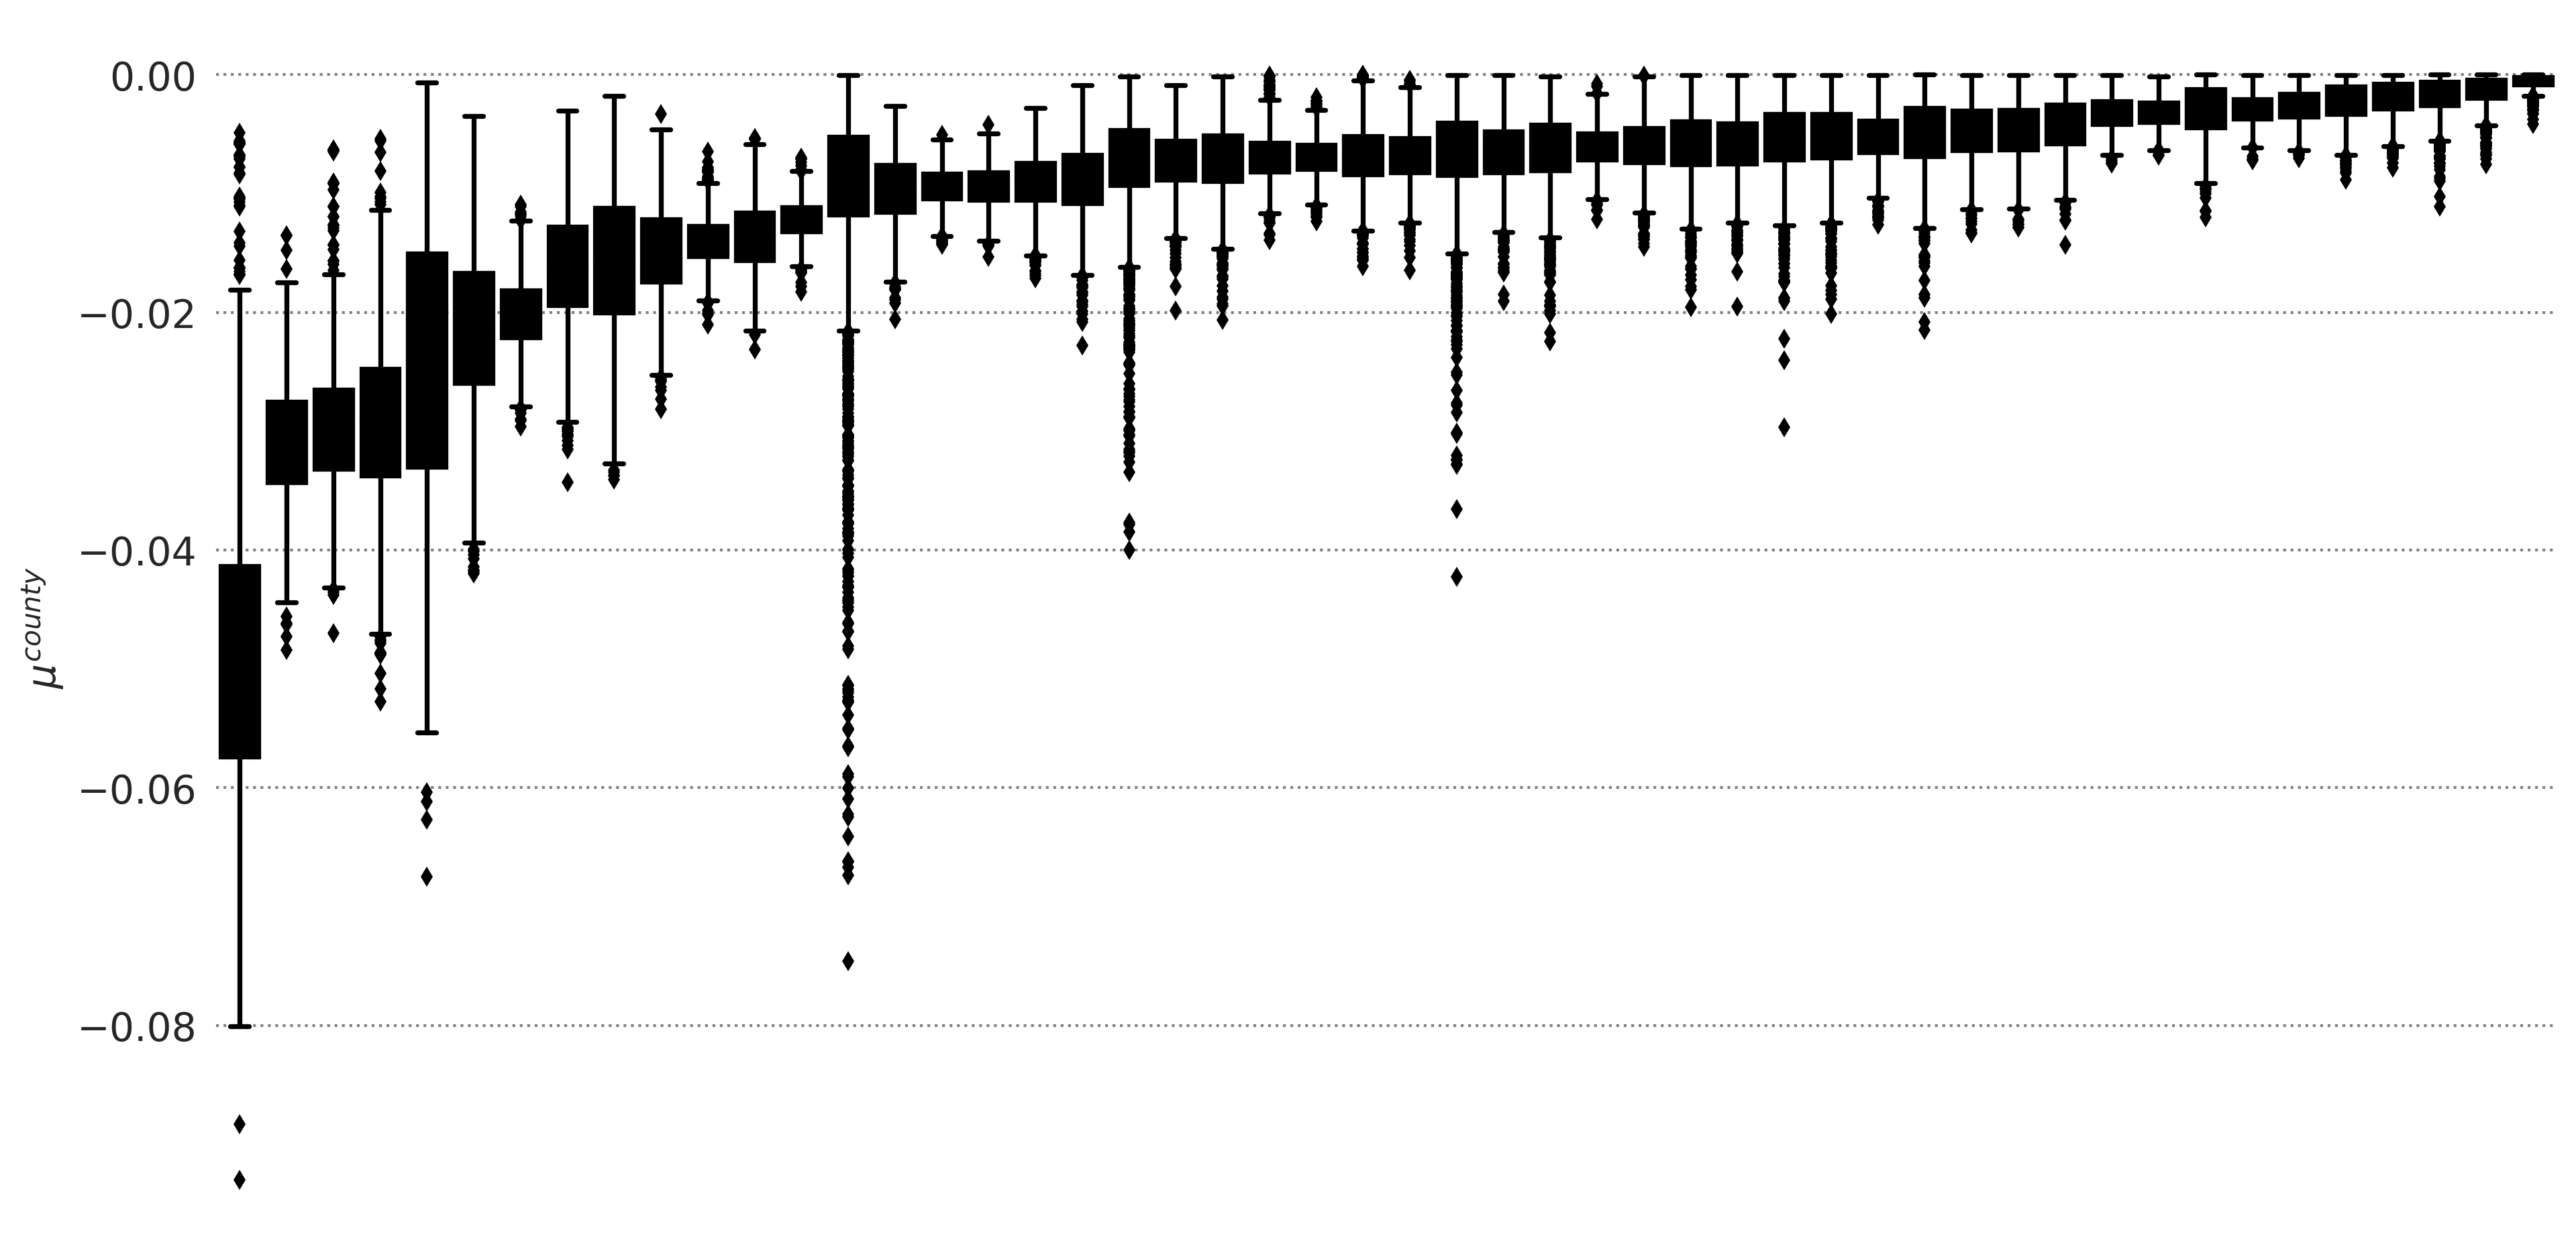
\includegraphics[width=1\linewidth]{figures/BayCountyPlot_const.png}
  \label{fig:BayCountyPlot_const}
 \end{minipage}

\bigskip

\begin{minipage}[t]{.45\textwidth}
\centering
  \caption{Box plot of the the parameters $\mu^{county}$, representing the distributions of the mean parameter for county groupings.}
\end{minipage}\qquad
\begin{minipage}[t]{.45\textwidth}
\centering
  \caption{Box plot of the the parameters $\mu^{county}$, when all higher level mean parameters have a maximum of zero.}
\end{minipage}
\end{figure}

% new figure

\begin{figure}
\begin{minipage}{.45\textwidth}
  \centering
  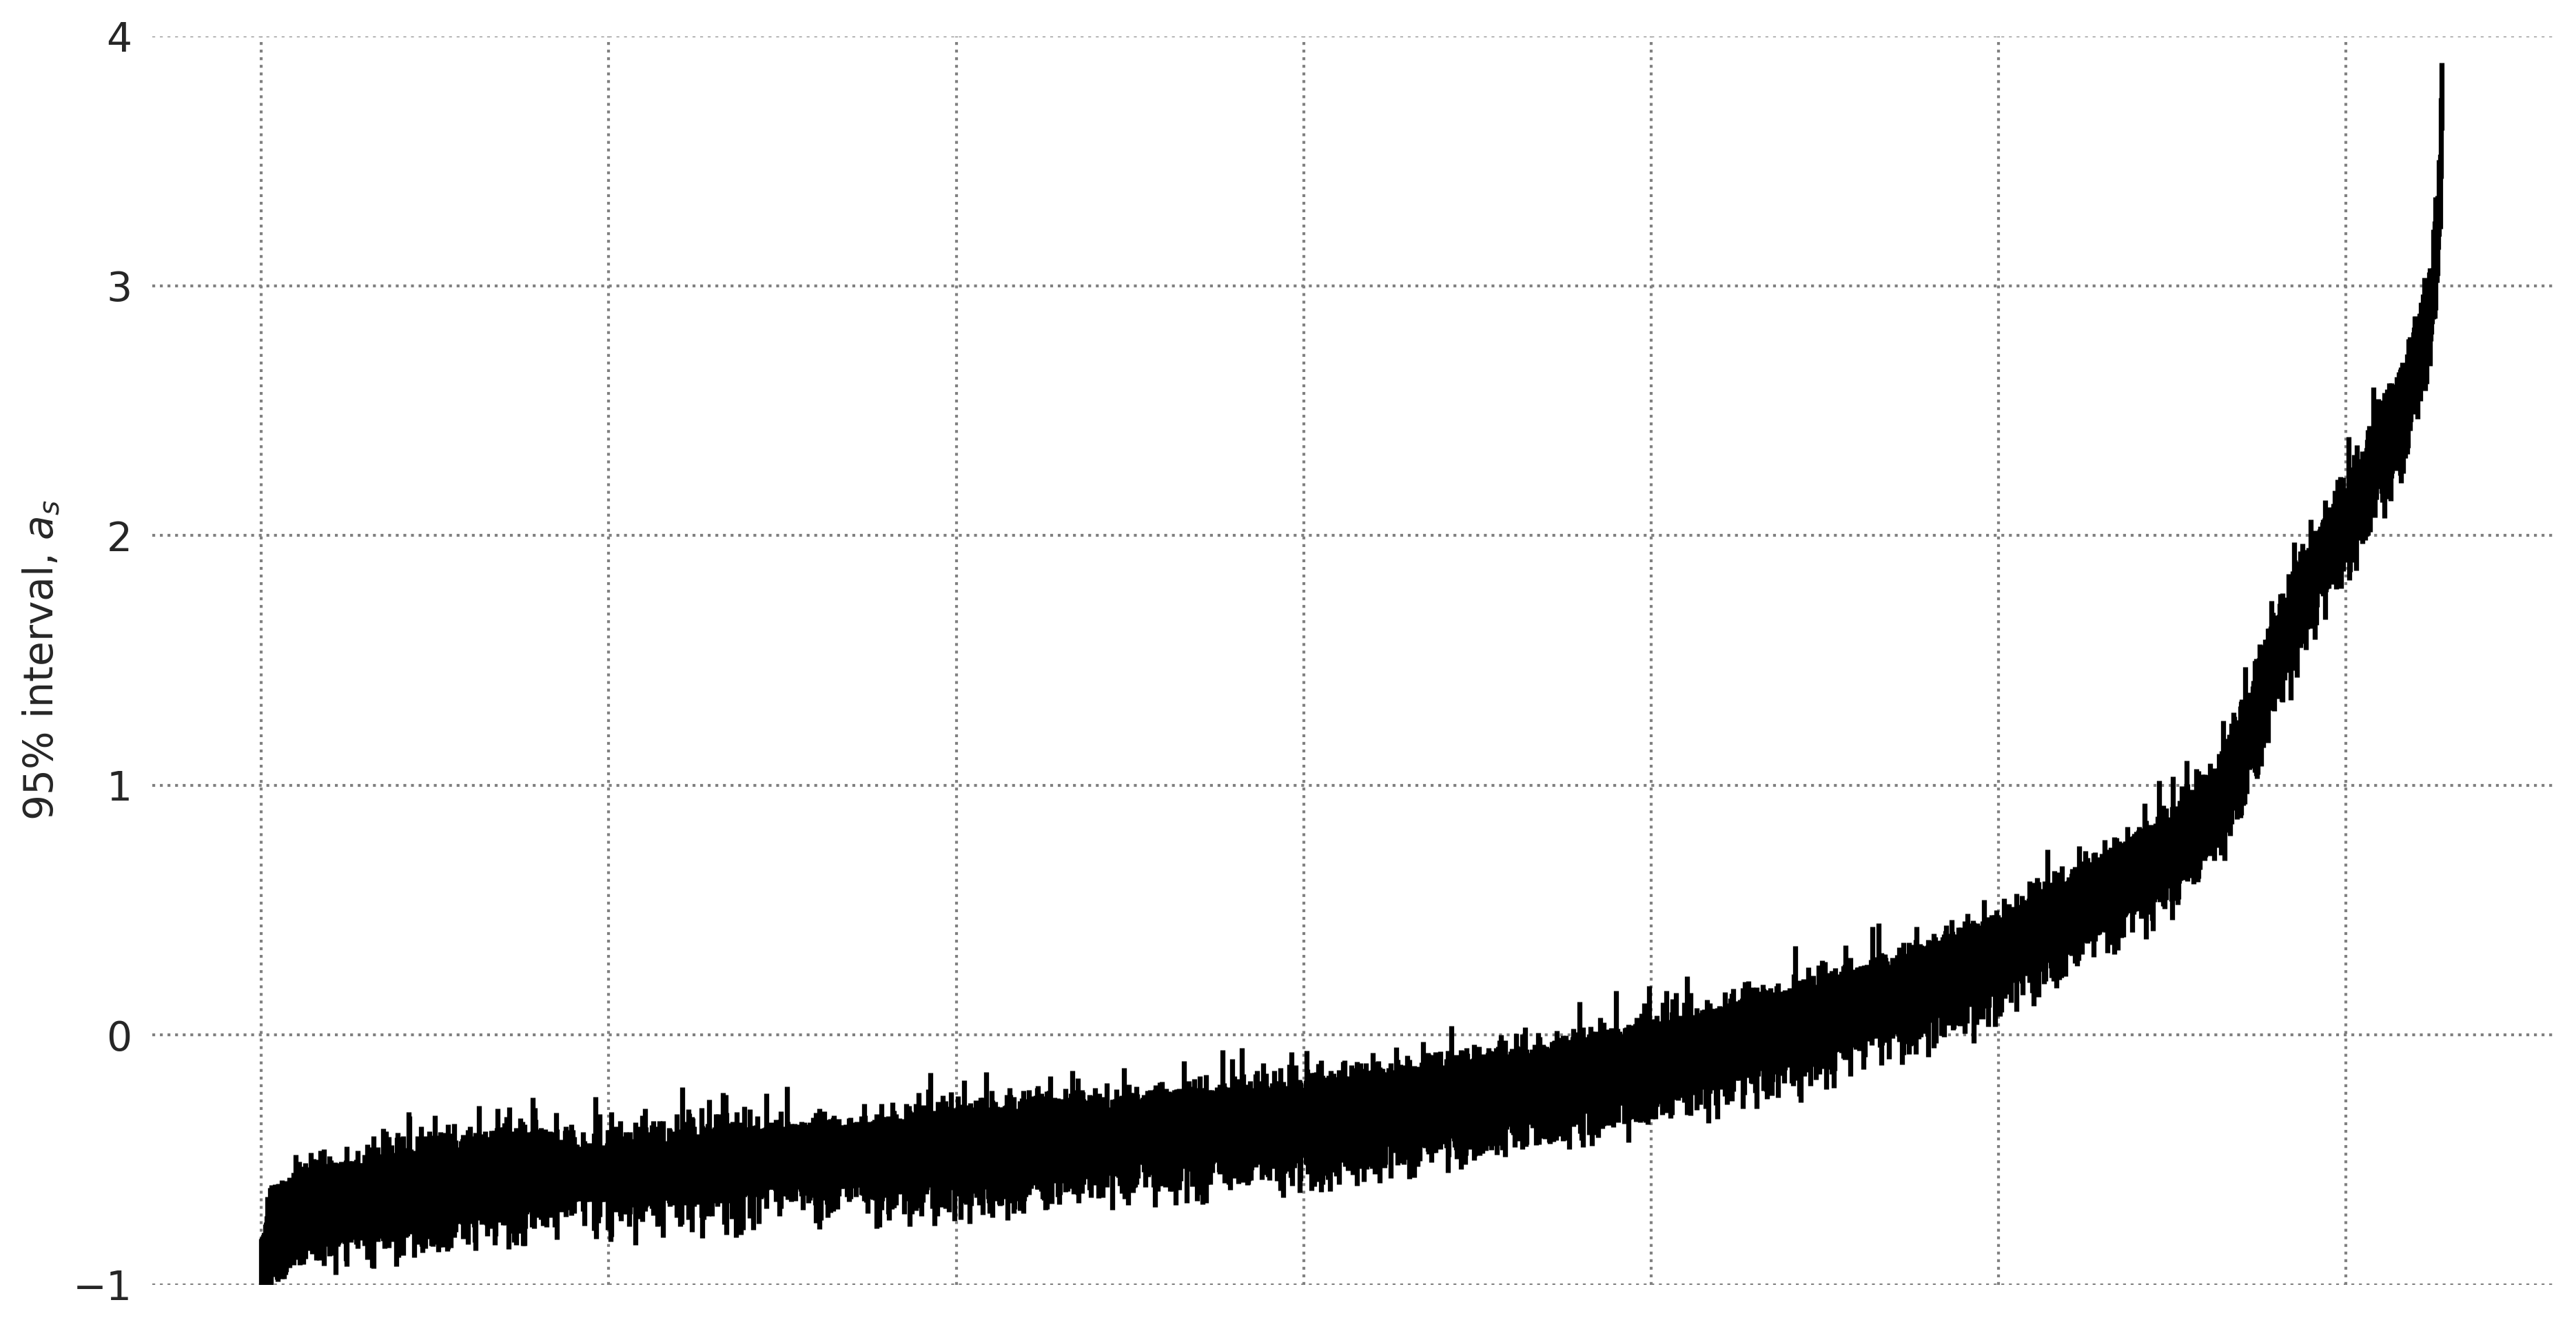
\includegraphics[width=1\linewidth]{figures/Bay_as.png}
  \label{sfig:Bay_as}
 \end{minipage}\qquad
\begin{minipage}{.45\textwidth}
  \centering
  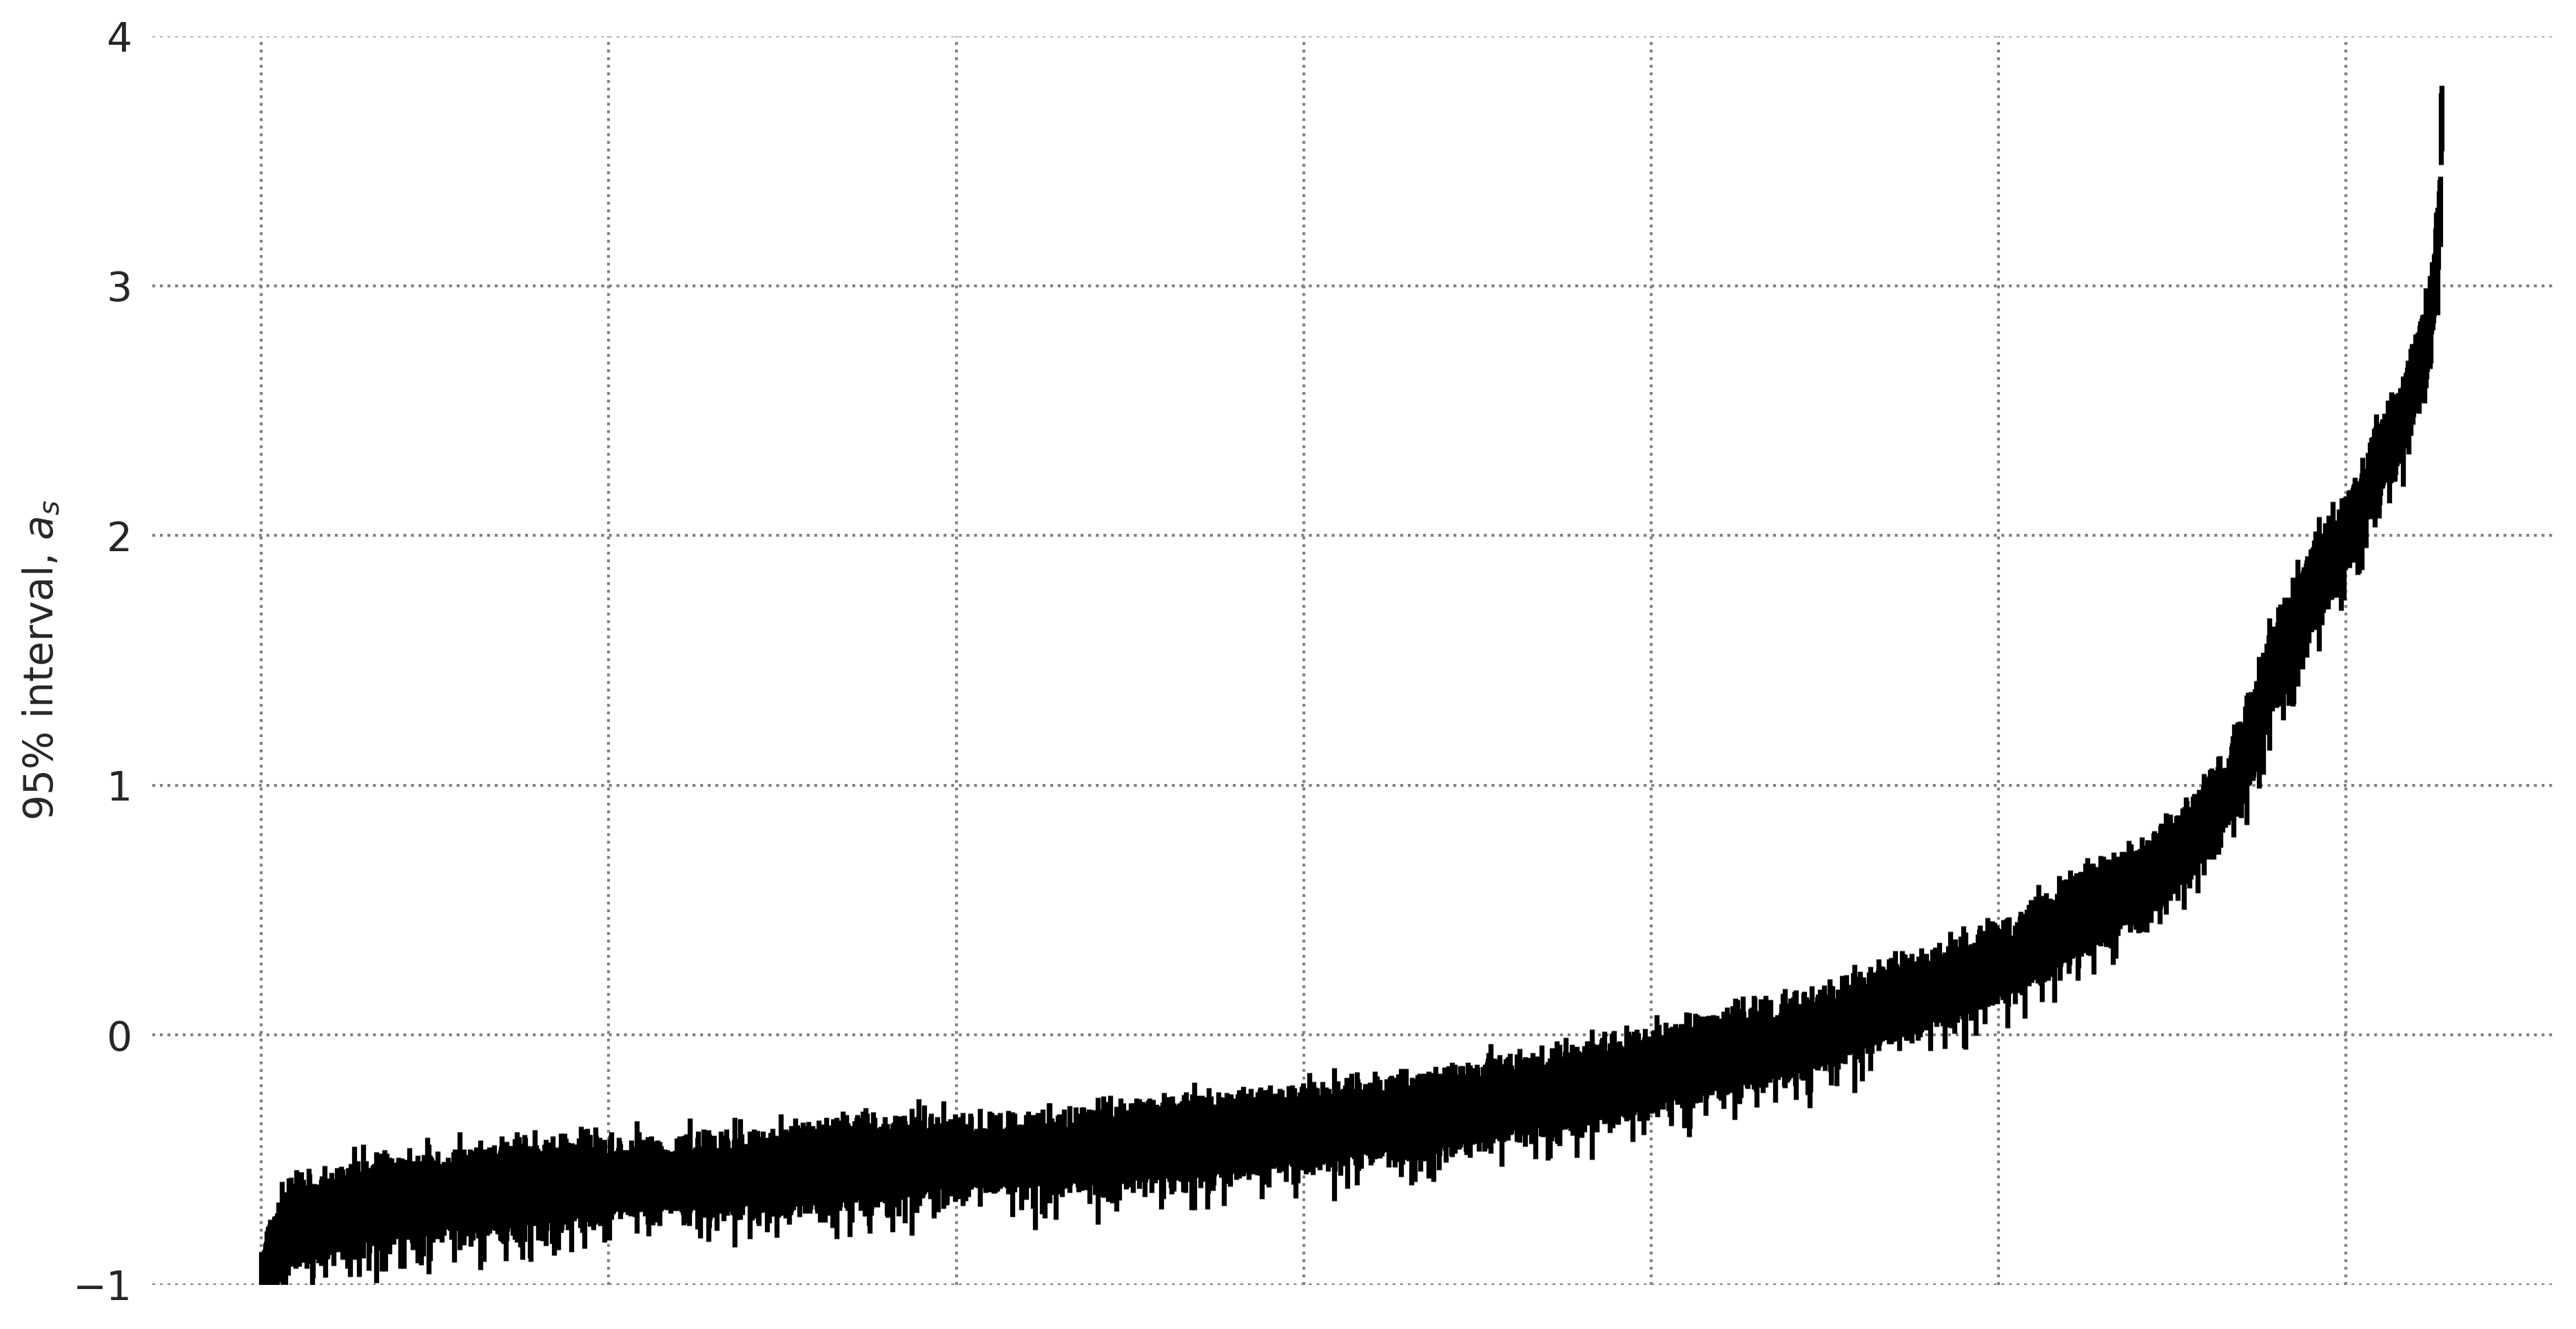
\includegraphics[width=1\linewidth]{figures/Bay_as_const.png}
  \label{sfig:Bay_as_const}
 \end{minipage}

\bigskip

\begin{minipage}[t]{.45\textwidth}
\centering
  \caption{95\% interval of the distributions of the system level intercept parameters, $a_s$.}
\end{minipage}\qquad
\begin{minipage}[t]{.45\textwidth}
\centering
  \caption{95\% interval of the distributions of the system level intercept parameters, $a_s$ when higher level mean parameters are constrained to have a maximum of zero.}
\end{minipage}
\end{figure}

% new figure

\begin{figure}
\begin{minipage}{.45\textwidth}
  \centering
  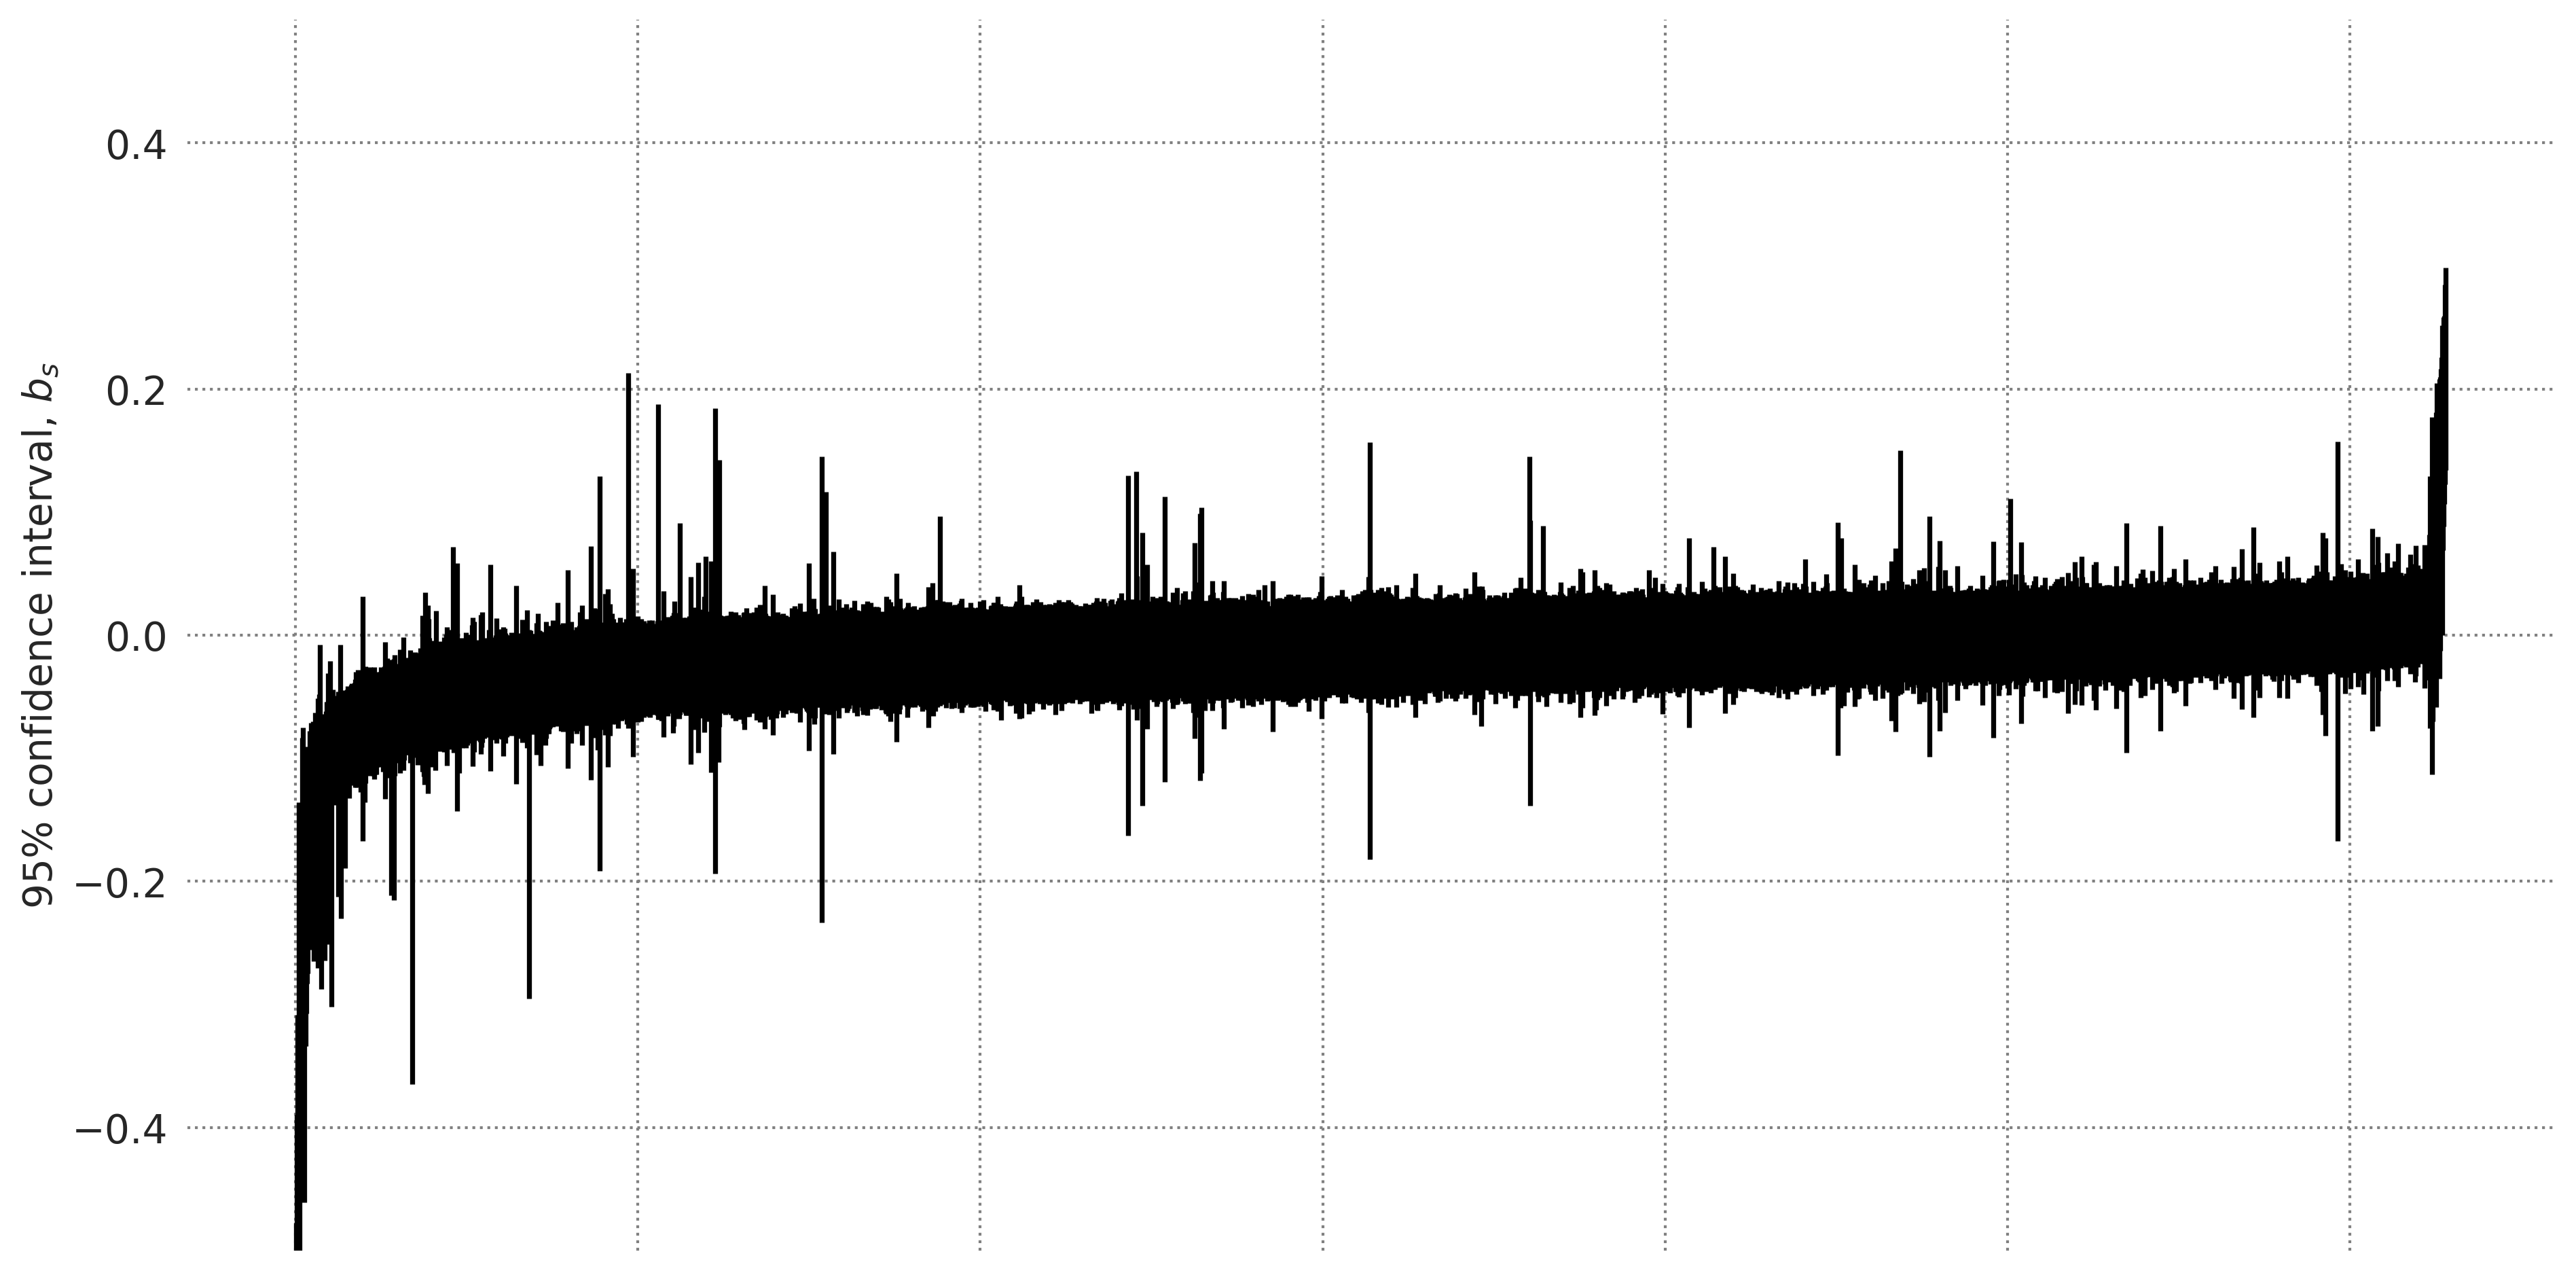
\includegraphics[width=1\linewidth]{figures/Bay_bs.png}
  \label{sfig:Bay_bs}
 \end{minipage}\qquad
\begin{minipage}{.45\textwidth}
  \centering
  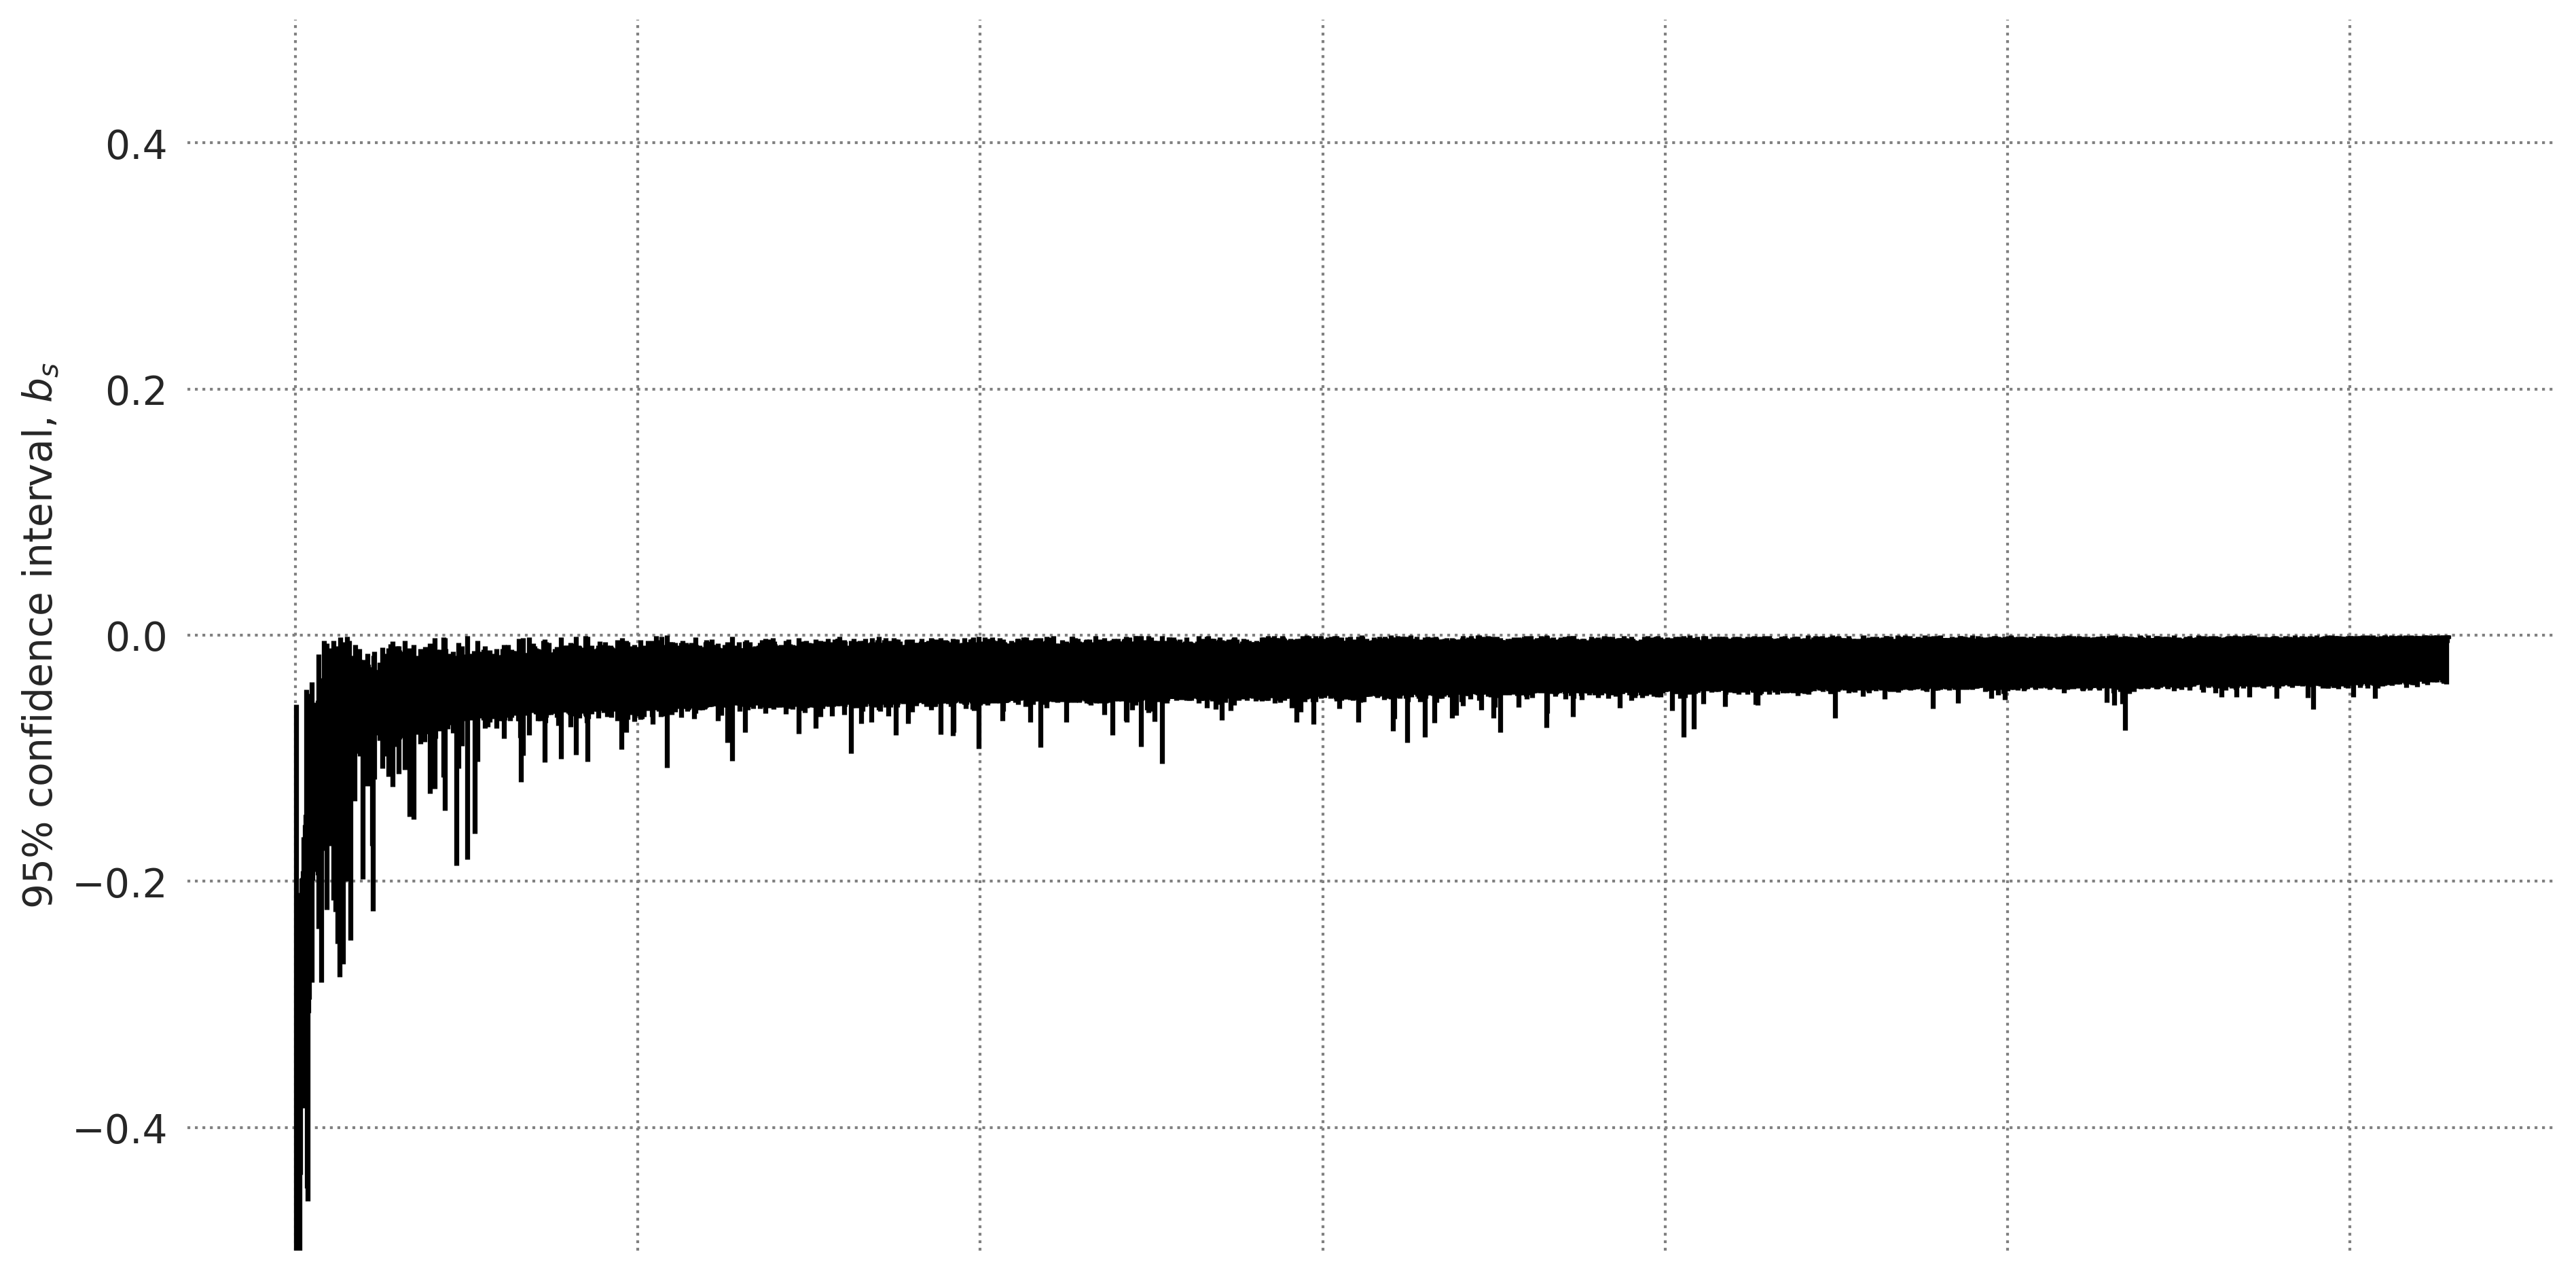
\includegraphics[width=1\linewidth]{figures/Bay_bs_const.png}
  \label{sfig:Bay_bs_const}
 \end{minipage}

\bigskip

\begin{minipage}[t]{.45\textwidth}
\centering
 \caption{95\% interval of the distributions of the system level slope parameter, $b_s$}
\end{minipage}\qquad
\begin{minipage}[t]{.45\textwidth}
\centering
  \caption{95\% interval of the distributions of the system level slope parameter, $b_s$}
\end{minipage}
\end{figure}


%\begin{figure}[!htb]
%\begin{minipage}{.48\textwidth}
%  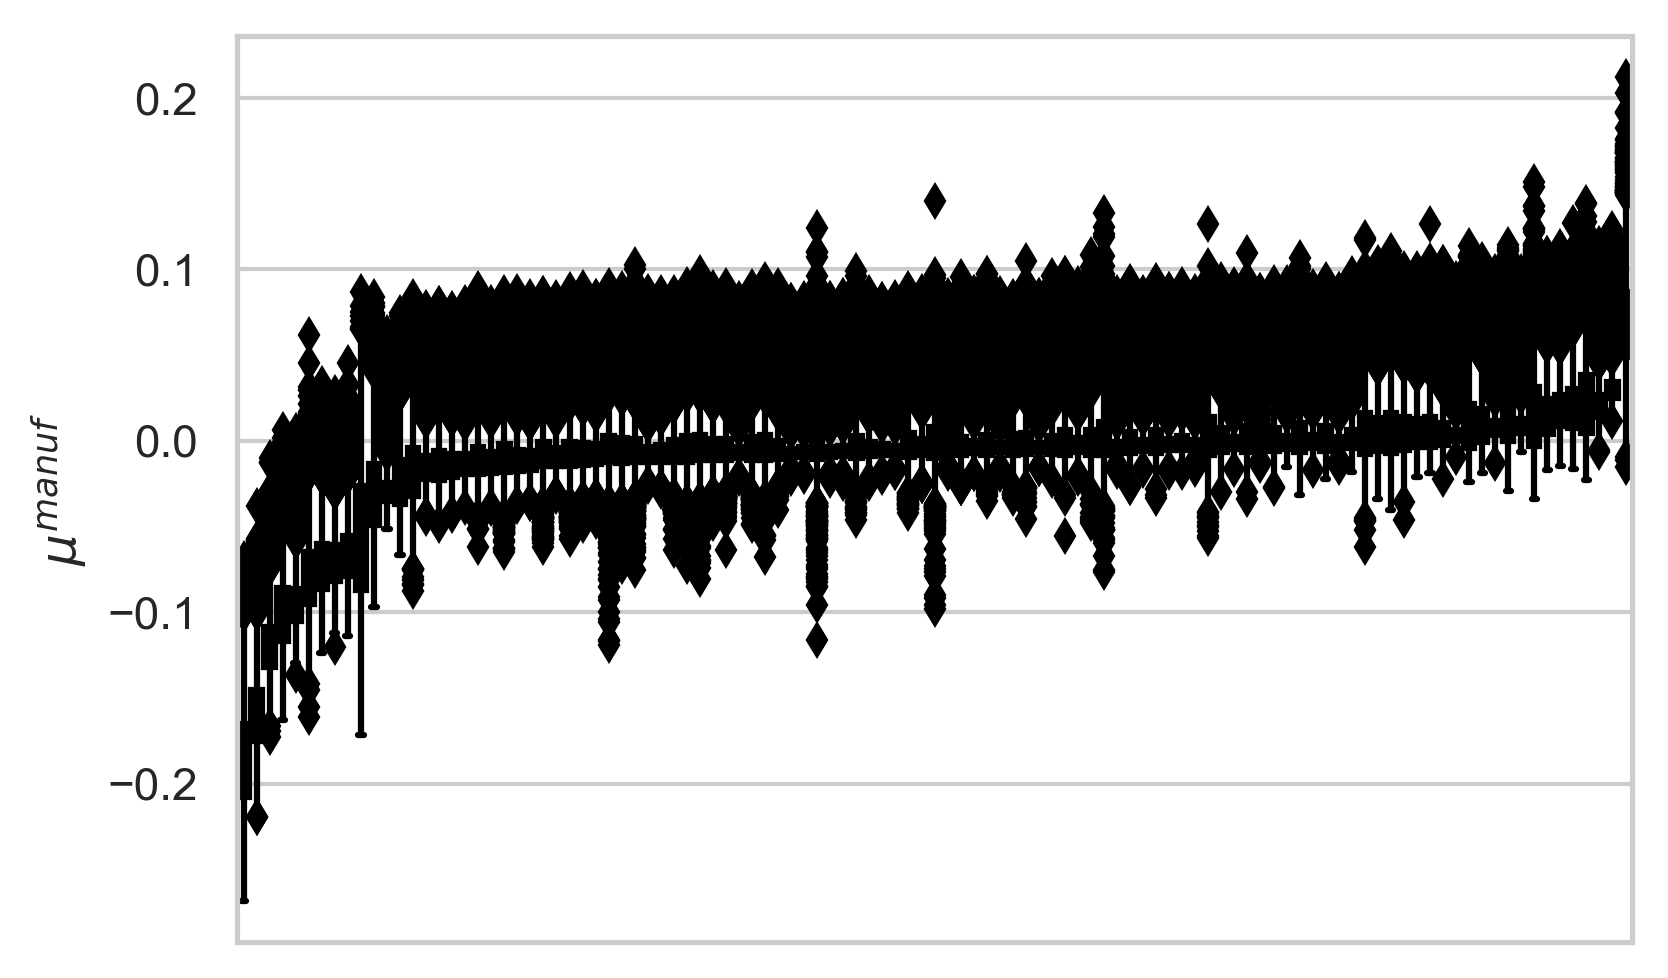
\includegraphics[width=1\linewidth]{figures/BayManPlot.png}
%  \caption{Box plot of the the parameters $\mu^{manuf}$, representing the distributions of %the mean parameter for manufacturer groupings.}
%  \label{sfig:BayManPlot}
%\end{minipage}\hfill
%\begin{minipage}{.48\textwidth}
%  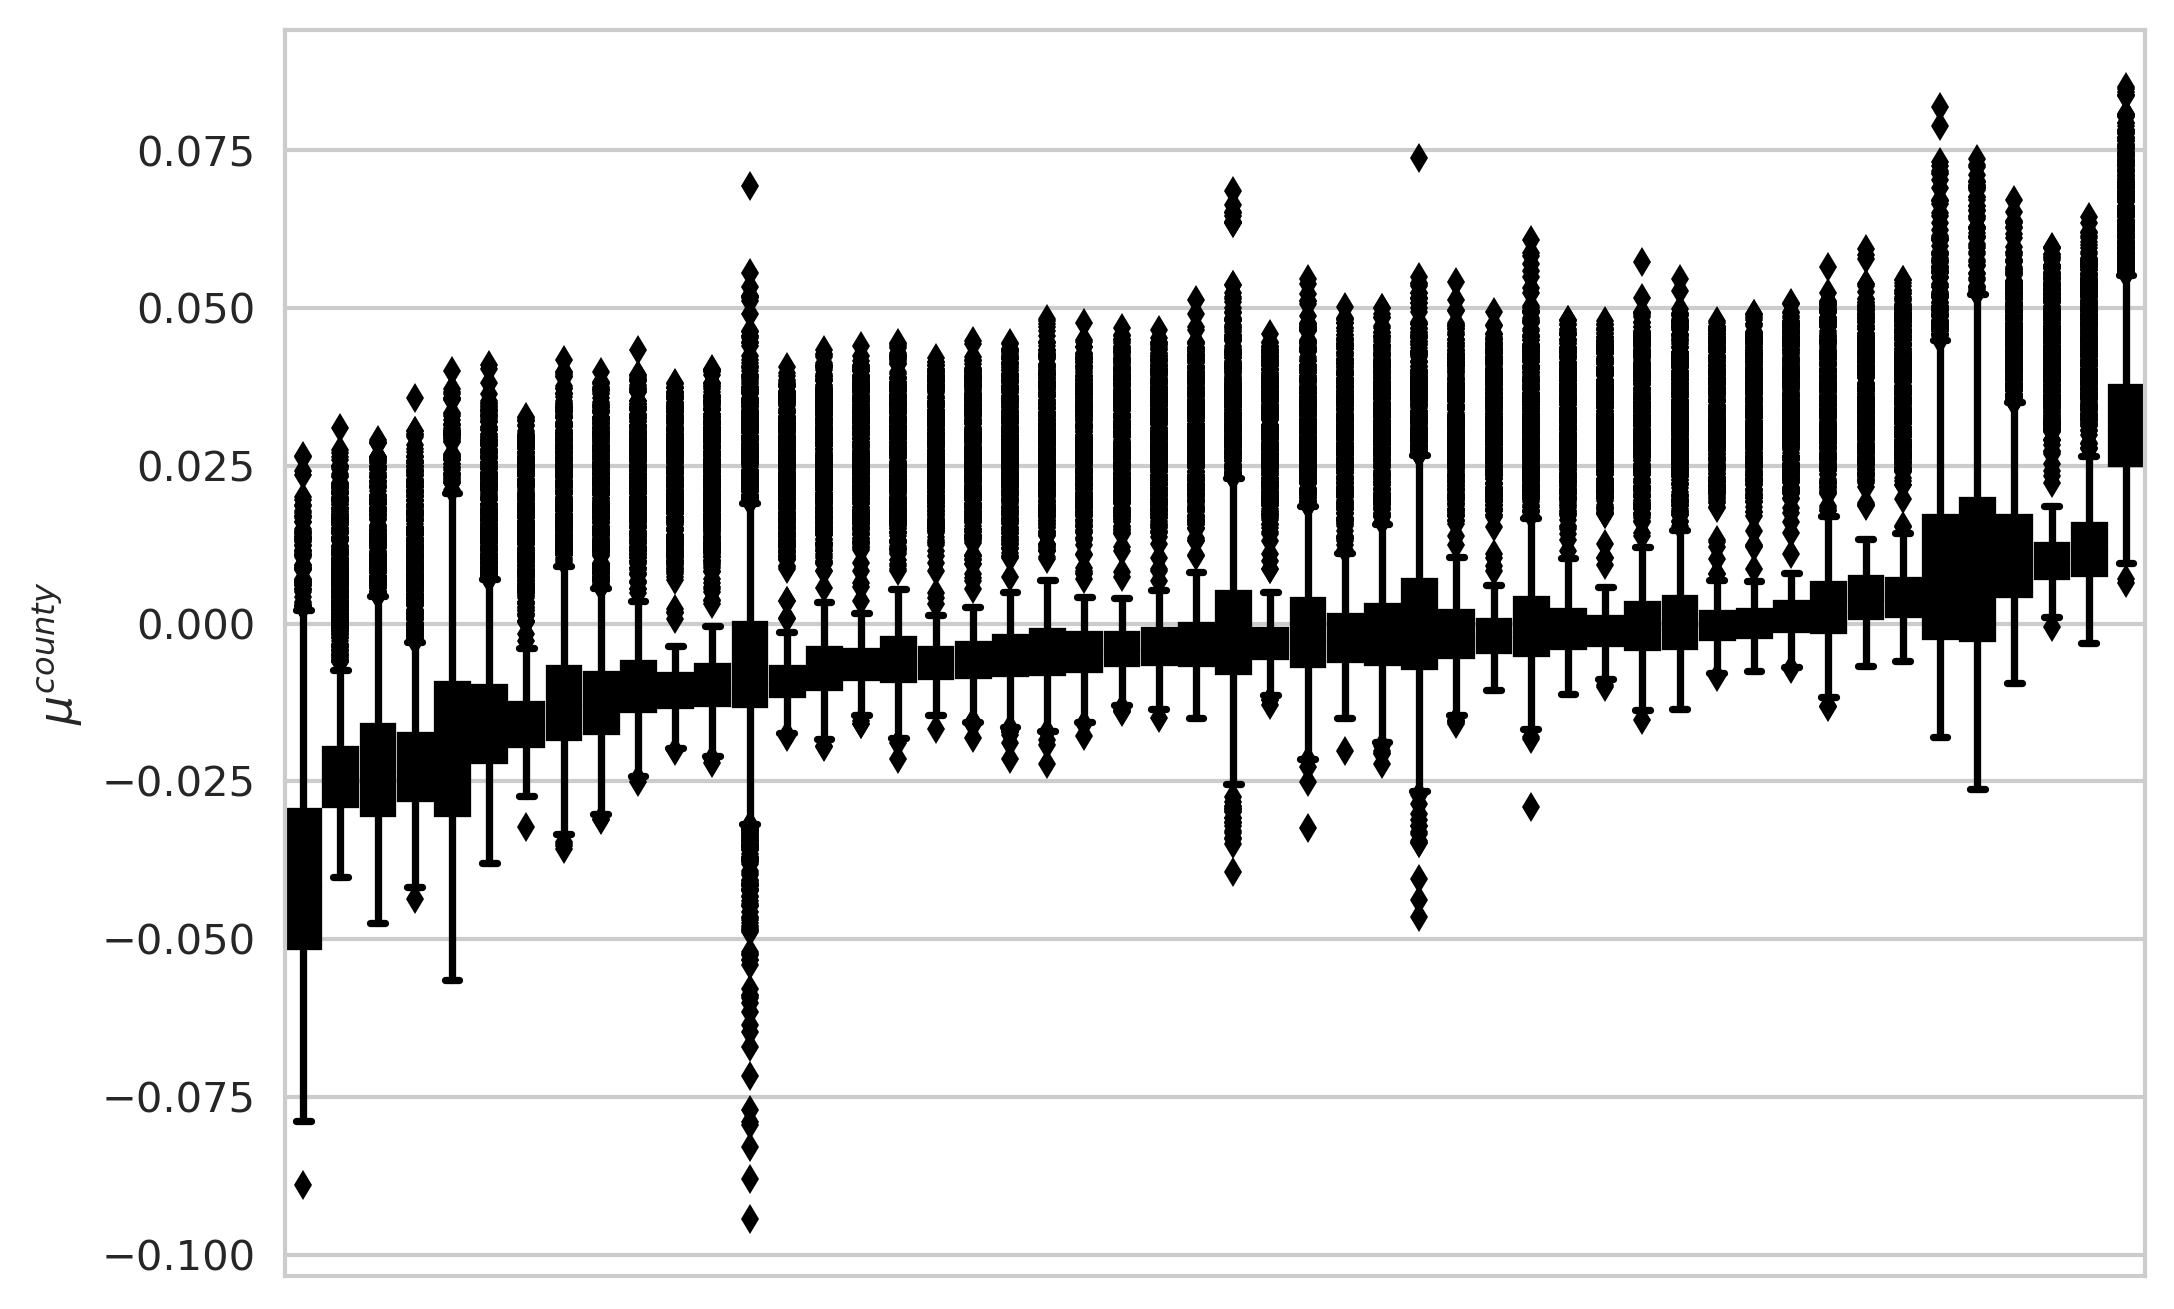
\includegraphics[width=1\linewidth]{figures/BayCountyPlot.png}
%  \caption{Box plot of the the parameters $\mu^{county}$, representing the distributions of the mean parameter for county groupings.}
%  \label{sfig:BayCountyPlot}
%\end{minipage}\hfill
%\begin{minipage}{.48\textwidth}
%  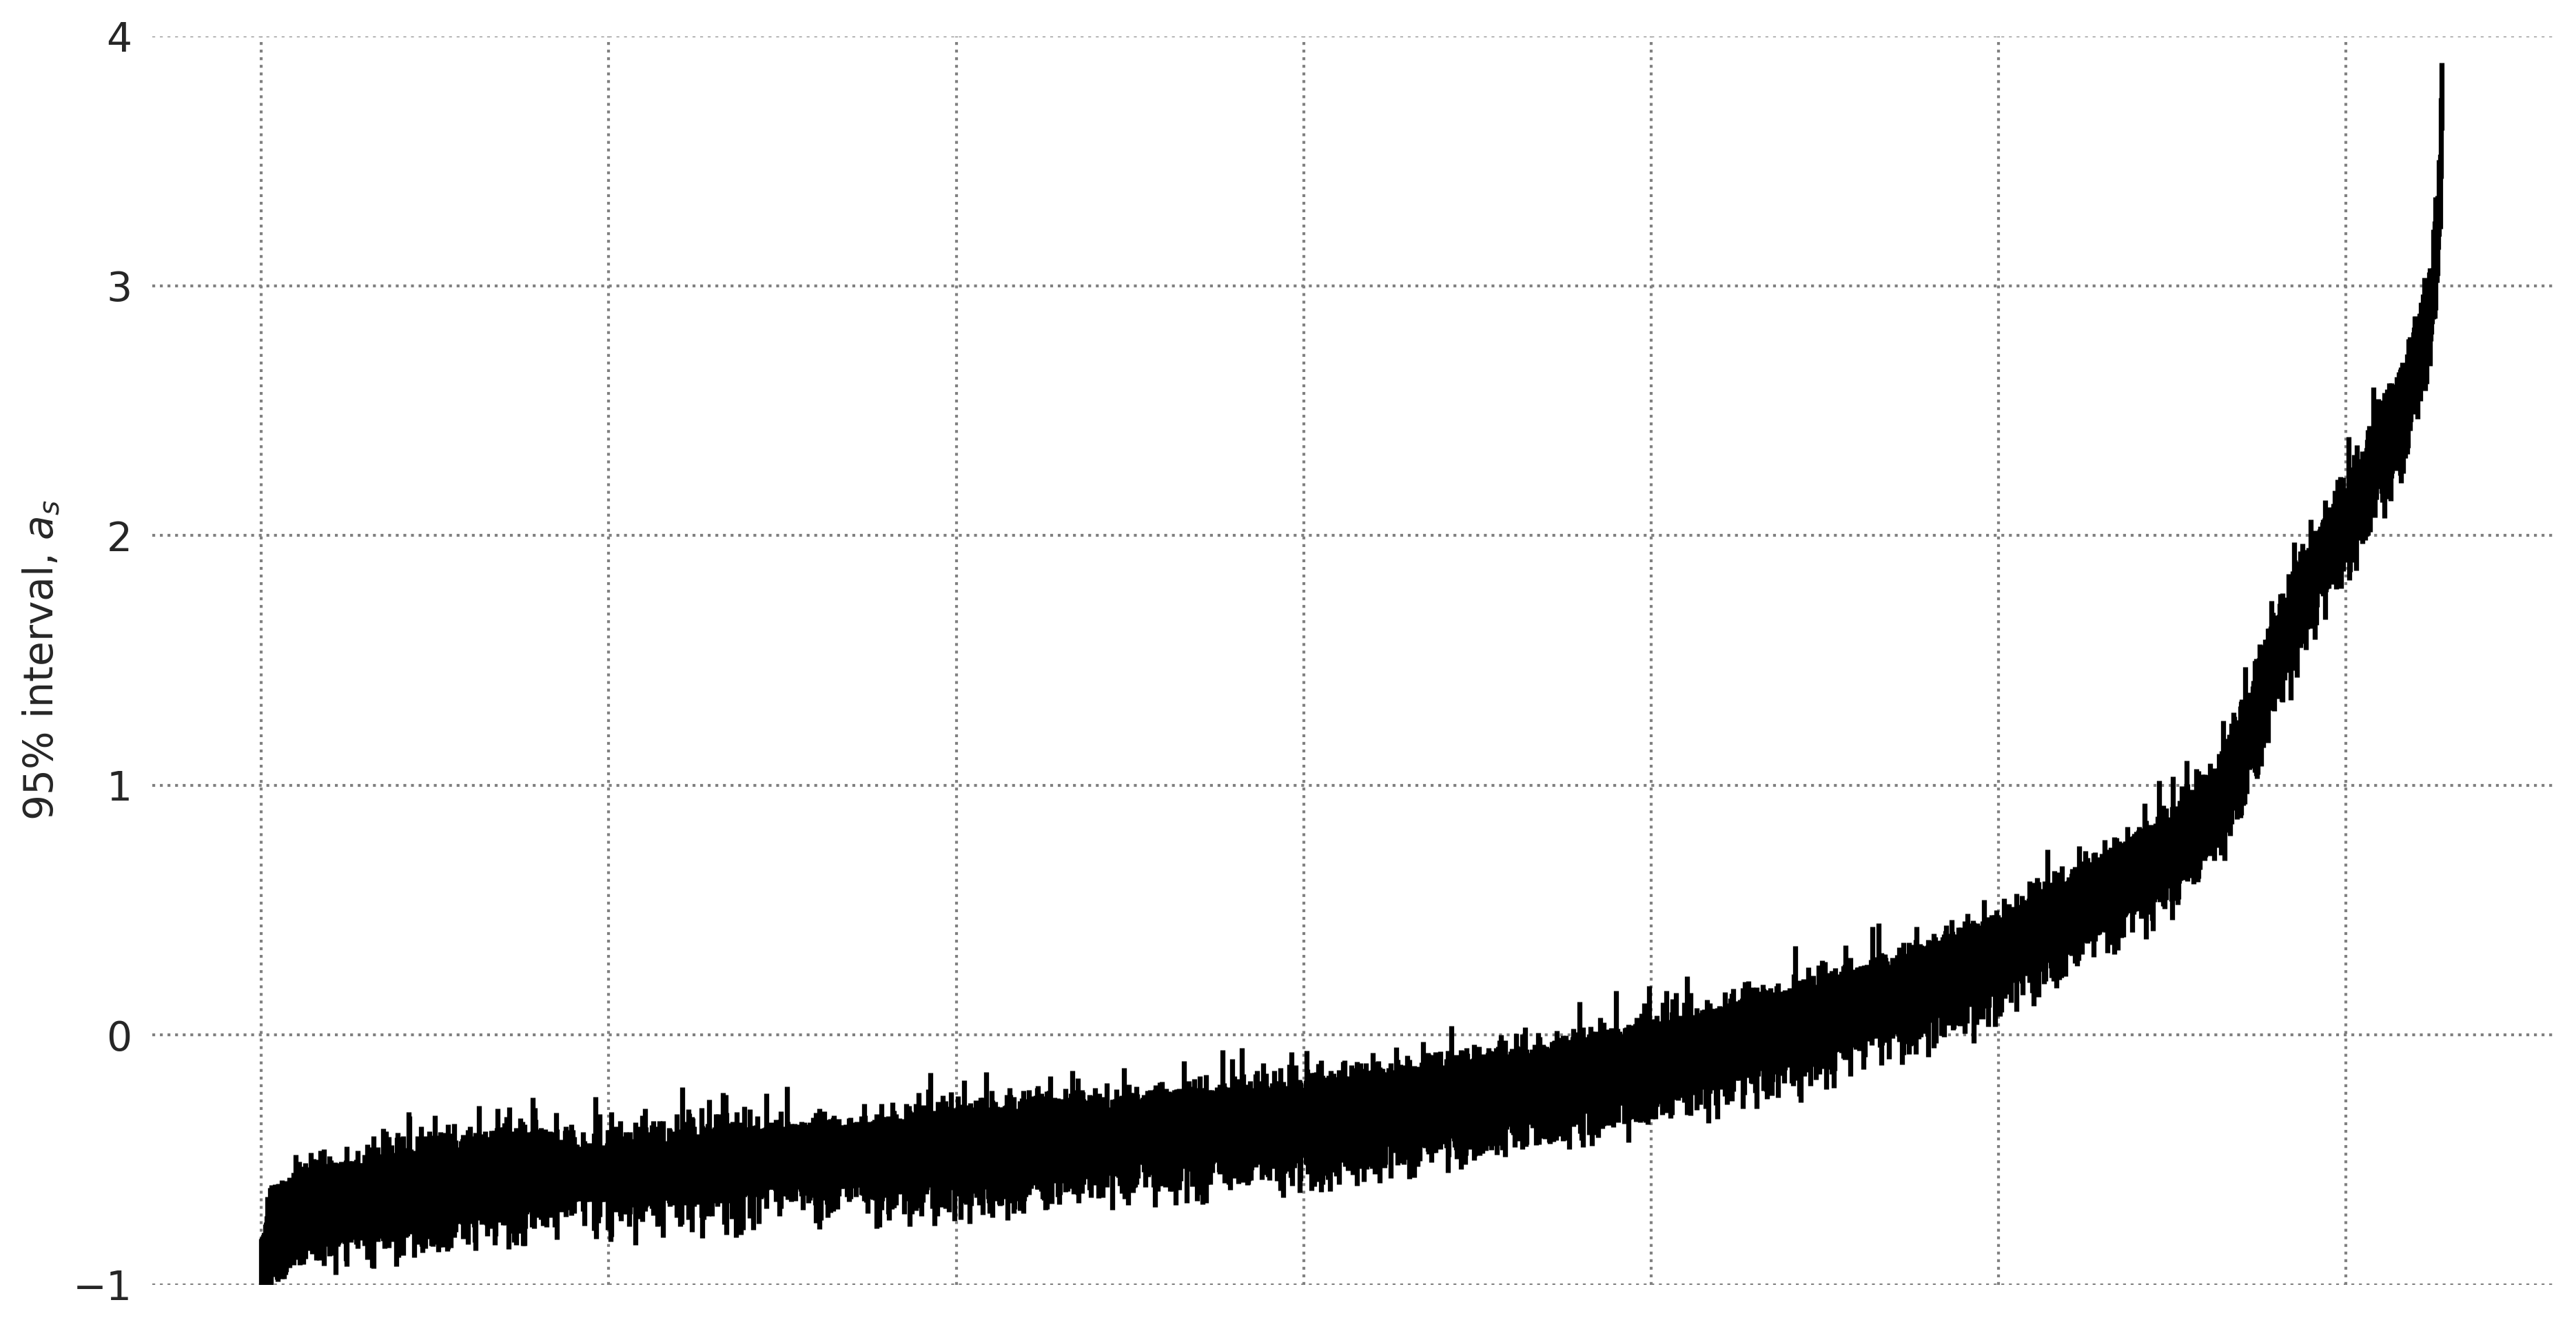
\includegraphics[width=1\linewidth]{figures/Bay_as.png}
%  \caption{95\% interval of the distributions of the system level intercept parameters, $a_s$.}
%  \label{sfig:Bay_as}
%\end{minipage}\hfill
%\begin{minipage}{.48\textwidth}
%  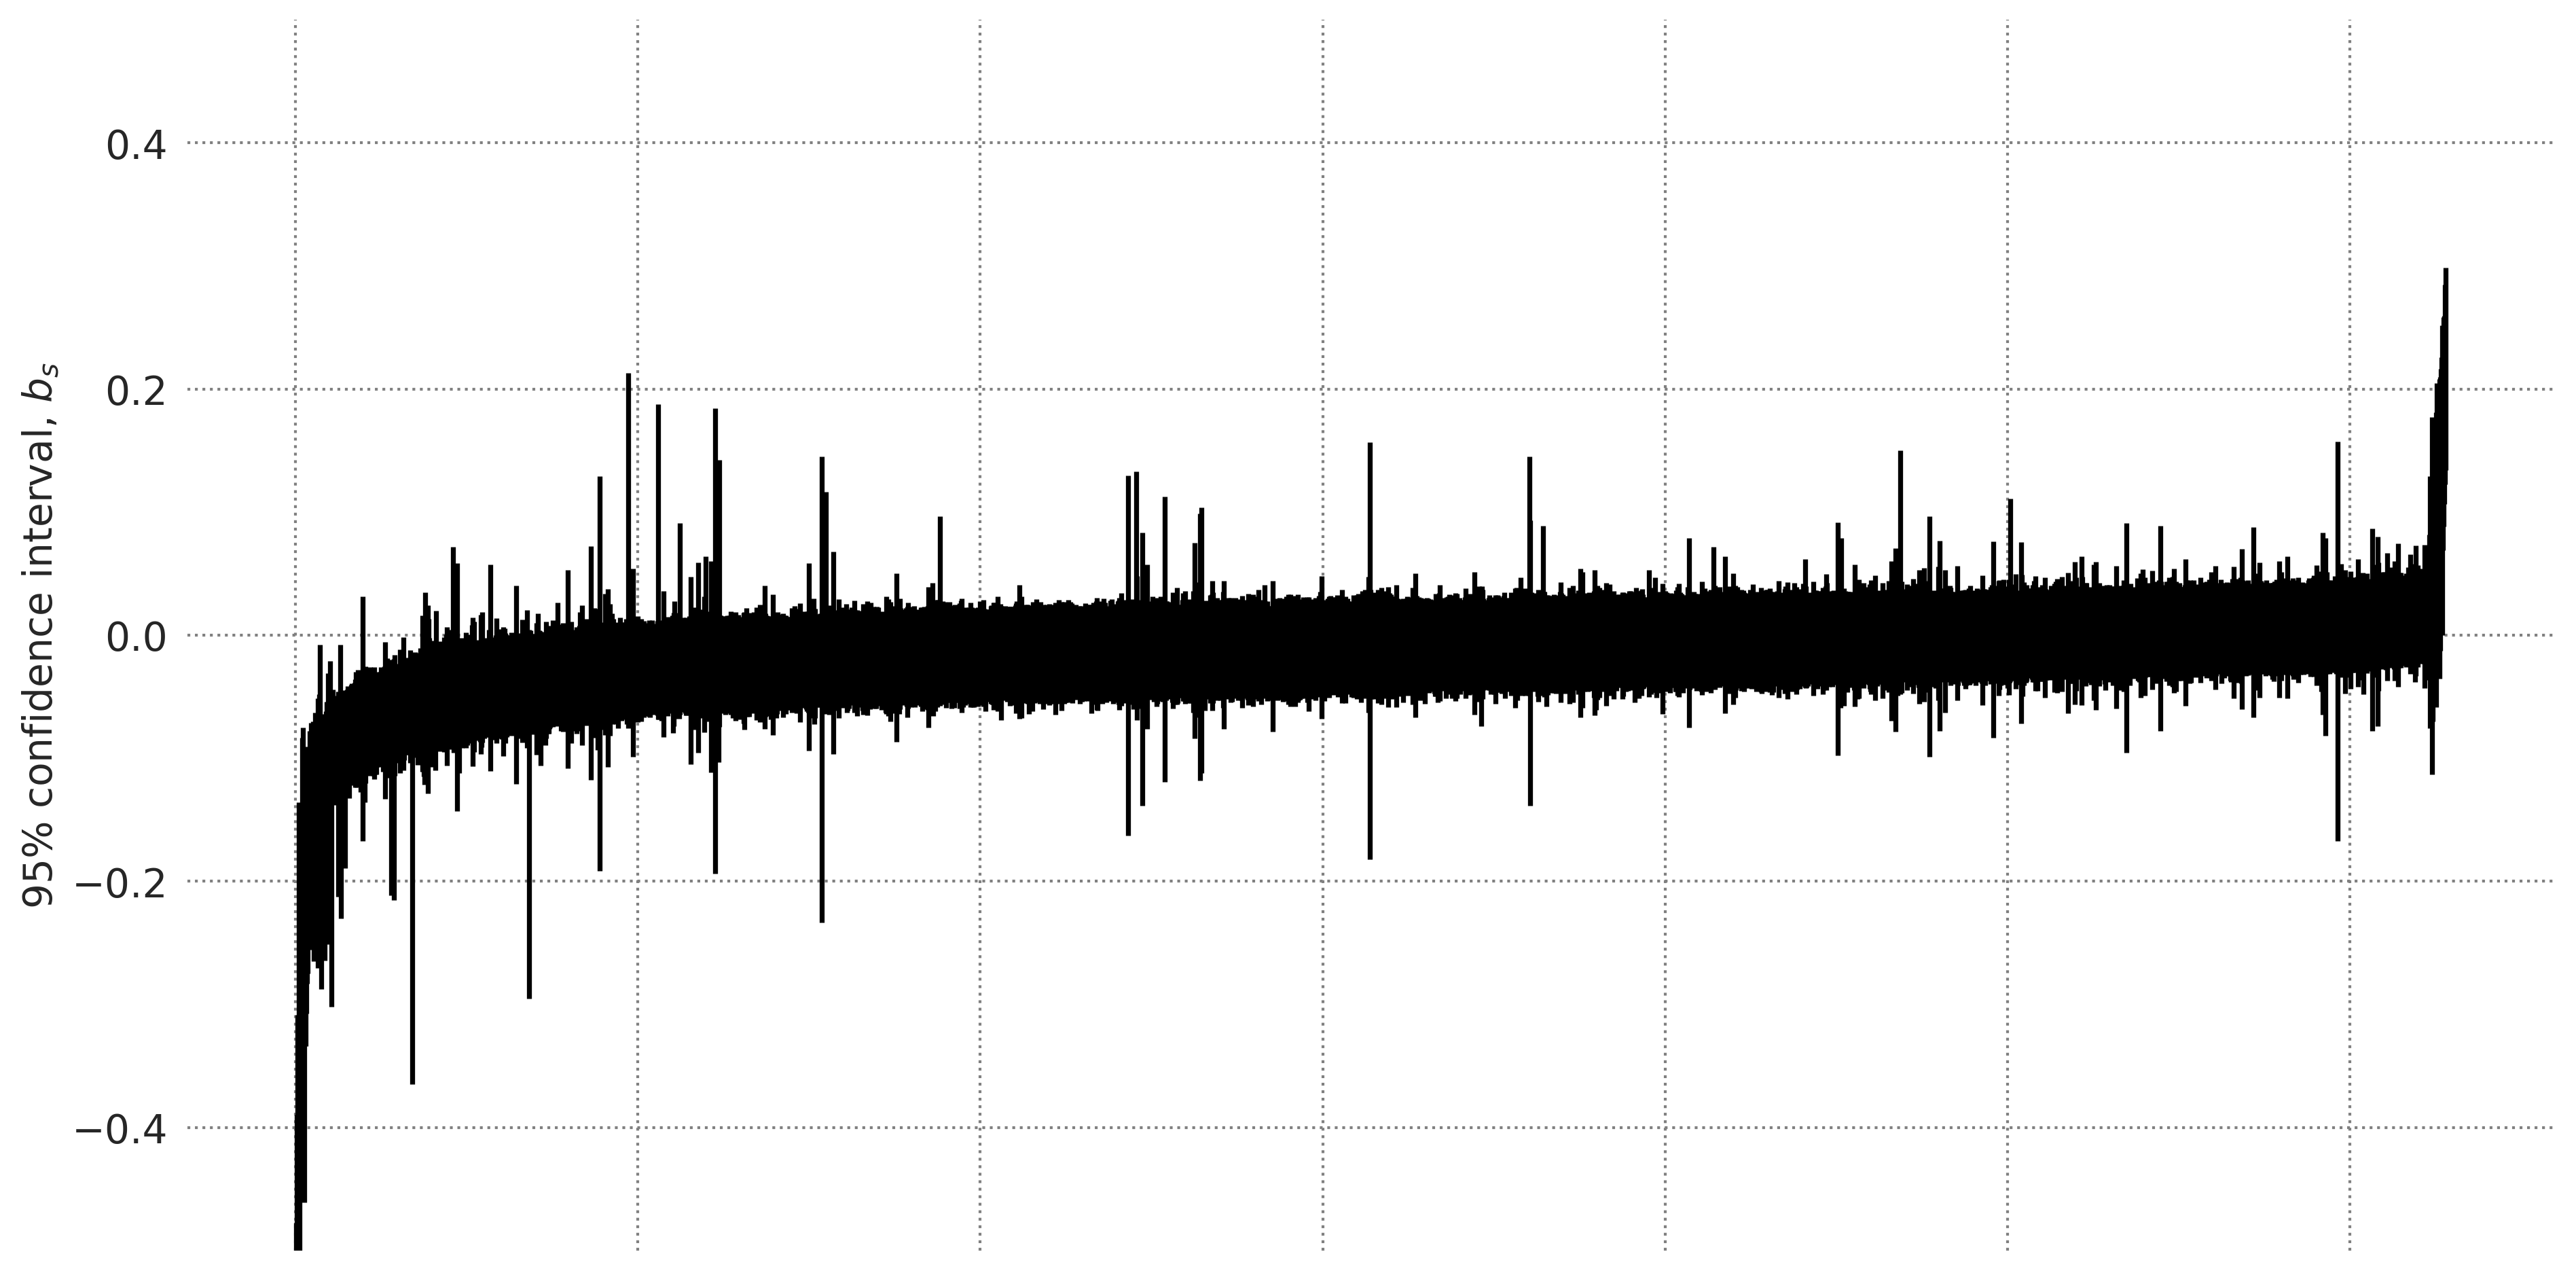
\includegraphics[width=1\linewidth]{figures/Bay_bs.png}
%  \caption{95\% interval of the distributions of the system level slope parameter, $b_s$}
%  \label{sfig:Bay_bs}
%\end{minipage}\hfill
%\caption{Simulated distribution of coefficients}
%\label{fig:coeff_sim}
%\end{figure}

\section{Discussion and Conclusion}

Because of the dramatic price declines in solar panels and the competitive pressure that western producers have faced, it has become common to hear in the industry that solar panels have become commodities. But in finance and economics, commodity has a specific meaning. Commodities of a certain grade need to be fungible: goods from different producers are interchangeable.

Historically, the commoditization of goods was a necessary condition for the establishment of sophisticated financial markets for those goods. The invention of grain elevators for mixing and thereby standardizing grain was a necessary precursor to the establishment of a futures markets with receipts of delivery traded on the Chicago Board of Trade \citep{cronon_natures_1992}. The abstraction between producer and end purchaser of goods was necessary for the functioning of these markets. A trader could fulfill a promise to deliver grain of a certain grade by simply buying it on the market or with cash settlement, rather than having produced it oneself.

If solar panels truly have become commodities, it would have meaningful and substantial implications for the solar power industry. For example, financial instruments could arise providing developers of solar power plants or solar panel retailers the ability to hedge price uncertainty in panels and guarantee supplies for projects with long lead times. Particularly relevant to the current environment would be trade policy. Trade restrictions on panels from specific countries, like the current US tariffs on Chinese produced panels, would presumably be less effective. Fungible panels from China could easily be sold elsewhere, while similar panels from other countries supply the US market.

Yet the findings from this article strongly suggest that solar panels are not commodities. In particular, I find that the salient property of quality varies substantially between producers. Because solar power is a distributed technology, where assets can be owned by individual homeowners, businesses and other other organizations that do not have the resources to judge quality, the issue of asymmetric information may then enter the market.

From a descriptive understanding of the market, I identify a high information type owner (third-party owners) and low information type owner (host-owners) of solar power assets. Then, from the basic theory of asymmetric information of quality, I explore two testable implications. I find that, as the theory would predict, high information owners are able to attain higher-quality panels. With about 90 percent probability, I also find that the cost of solar panel systems owned by high-information types is more highly correlated with quality, as theory would also suggest.

The market for solar panels and solar panel systems is however still young and dynamic. One of the advantages of the linear mixed-effects models and the hierarchical models is that we can also get an idea of the degree of differentiation in quality between different manufacturers. It appears that a relatively small tail of producers accounted for the worst quality panels, while the majority of panels had similar quality. The market for solar panels is still relatively young, and if low-quality producers either are forced to exit the market or improve their quality to match standards in the industry, then it is possible that solar panels could indeed become commodities in the future, with associated implications for pricing, competition and financing.

\bibliographystyle{chicago}
\bibliography{solar_prod}

%\FloatBarrier

%\appendix
%\section{Appendix: Tables}


\end{document}
